\setcounter{subsection}{0} 
\part{Data - Monte Carlo comparison}
This thesis concludes with a comparison of the obtained $\bar{n}$ candidates cluster variables against those obtained from data. The dataset is the latest available from Belle II data production, corresponding to an integrated luminosity of $358.27 fb^{-1}$. The same selections achieved in $q\bar{q}$ are applied, in both ISR and NO ISR cases. Since the goal is to assess Data/MC agreement for cluster variables from the analysis -rather than maximize signal selection efficiency- these variables are compared within the signal region [0.8, 1.2] GeV, without sideband subtraction.

\subsection{Recoil mass in data}
First, the recoil mass distribution in data is studied by analyzing the angular distributions of reconstructed protons. The resulting distribution (no ISR case) is shown in Fig.~\ref{fig:recM_nog_data_pre}.

\begin{figure}[H]
    \centering
    
\includegraphics[width=0.49\textwidth]{nbar_DATA/images/recoil_mass_data_precutnog}
        
\includegraphics[width=0.49\textwidth]{nbar_DATA/images/recoil_mass_data_precutisr}
    \caption{Recoil mass distribution in data. NO ISR case (left) and ISR case (right).}
    \label{fig:recM_nog_data_pre}
\end{figure}

Unlike the Monte Carlo simulation, in data no signal peak is observed at the anti-neutron mass.A completely different behavior is observed, with a prominent structure at low recoil mass values, suggesting that some particles in the recoil system $p \pi^-$ are not properly reconstructed.
$\\$
Since the proton has the strictest selection criteria ($protonID > 90\%$), it is now investigated in detail. To properly select the signal in the recoil mass distribution, the 2D distribution $\cos(\theta)$ vs momentum for reconstructed protons is studied.Several background sources not included in the Monte Carlo $q\bar{q}$ cocktail could arise. The obtained distribution is shown in Fig.~\ref{fig:proton_costheta_p}.
\begin{figure}[H]
    \centering
    
\includegraphics[width=0.49\textwidth]{nbar_DATA/images/proton_costheta_p}
     
\includegraphics[width=0.49\textwidth]{nbar_DATA/images/proton_costheta_p_isr}
    \caption{2D $\cos(\theta)$ vs momentum distribution in data. NO ISR case (left) and ISR case (right). Please, zoom in.}
    \label{fig:proton_costheta_p}
\end{figure}

Two structures are observed in the backward region ($cos(\theta) < -0.45$): one at proton momentum $p < 2$ GeV/c and one at $p \sim 3{-}4$ GeV/c. Furthermore, a strip structure is observed in the forward region ($cos(\theta) > 0.85$) across the full proton momentum range.
$\\$
Even if a strong selection on proton list has been performed, such as that on \emph{protonID}, insufficient coverage in the backward and deep forward regions prevents proper proton selection, allowing multiple background sources to arise. For example background sources like the following one:

\begin{center}
$e^+ e^- \rightarrow e^+ e^-$ \hspace{2cm} $e^+ e^- \rightarrow \pi^+ \pi^-$,
\end{center}
where the positive track could be misidentified as the reconstructed proton in the backward-forward regions. 
$\\$
Therefore, a further selection can be performed on reconstructed proton $cos(\theta)$ variable, such as that $-0.45<cos(\theta)<0.85$, in order to exclude the structures observed in Fig.~\ref{fig:proton_costheta_p}. The following recoil mass distribution is shown in Fig.~\ref{fig:recM_nog_data_post}.
\begin{figure}[h]
    \centering
    
\includegraphics[width=0.49\textwidth]{nbar_DATA/images/recoil_mass_data_postcutnog}
      
\includegraphics[width=0.49\textwidth]{nbar_DATA/images/recoil_mass_data_postcutisr}
    \caption{Recoil mass distribution in data. NO ISR case (left) and ISR case (right). Cut $-0.45<cos(\theta)<0.85$ applied, on the reconstructed protons.}
    \label{fig:recM_nog_data_post}
\end{figure}
A structure at the anti-neutron mass is now observed, confirming that the discussed structures caused incorrect reconstruction of the recoil system. 
$\\$
Therefore, the event selections adopted for the remaining data analysis are as follows:
\begin{enumerate}
\item Recoil system: $0 \ GeV/c^2 <recoil \ mass < 2 \ GeV/c^2$ and in ECL acceptance;
\item $\bar{n}$: neutral clusters from ECL and number of hits $> 10$ and energy $<3$ GeV;
\item $p$: $protonID > 0.9$ and $dr<1$ cm and $|dz|<3$ cm and $-0.45<cos(\theta)<0.85$;
\item $\pi^-$: $pionID > 0.1$ and $dr<1$ cm and $|dz|<3$ cm; 
\item $\alpha <0.10$ rad $\sim 5.73^\circ$;
\item No further charged particles in the Rest of Event (ROE).
\end{enumerate}

\subsection{Data/MC agreement}
The discussed $\bar{n}$ candidates cluster variables obtained in $q\bar{q}$ can be compared to those obtained from data. In order to perform the Data/MC agreement, the \textbf{pull variable} is adopted. It is a standardized metric used in high-energy physics to quantify discrepancies between observed data and Monte Carlo simulations. For a histogram i-th bin, the pull is defined as:
\begin{center}
$pull_i = \frac{N_{i,data} - N_{i,MC}}{\sqrt{\sigma^2_{i,data} + \sigma^2_{i,MC}}}$,
\end{center}
where $N_{i,\mathrm{data}}$ and $N_{i,\mathrm{MC}}$ represent the number of entries in the $i$-th bin, and $\sigma^2_{i,\mathrm{data}}$ and $\sigma^2_{i,\mathrm{MC}}$ are the corresponding uncertainties. With this definition, the pull variable corresponds to the difference between data and MC counts, weighted by the propagated uncertainty. 

The resulting distributions, without sidebands subtraction , are shown in Fig.~\ref{fig:dataMC_isr_nosid} (ISR case) and in Fig.~\ref{fig:dataMC_nog_nosid} (NO ISR case). Those with sidebands subtraction are shown in Fig.~\ref{fig:dataMC_isr_sid} (ISR case) and in Fig.~\ref{fig:dataMC_nog_sid} (NO ISR case).
$\\$
The Data/MC agreement plots reveal discrepancies between data distributions and $q\bar{q}$ Monte Carlo simulations. 
$\\$
The cluster energy shows good Data/MC agreement (within $2\sigma$ uncertainties) in both ISR and no-ISR cases across the full energy range, with and without sidebands subtraction.
$\\$
The cluster E1E9 shows discrepancies ($>2\sigma$) with and without sidebands subtraction, suggesting that more spread shower shapes must be accounted for. This is confirmed by discrepancies in the Zernike moments, indicating different shower shapes in data and simulation.
$\\$
The cluster E9E21 shows discrepancies ($>2\sigma$) without sidebands subtraction, but slightly better agreement afterward, confirming the trends observed in E1E9.
The cluster lateral momentum shows discrepancies before sidebands subtraction but better agreement afterward (within $2\sigma$ uncertainties across nearly the full range), without the structure at 0.3. This confirms the analysis effectively suppresses electromagnetic shower contributions, yielding an acceptable anti-neutron sample, even if the statistic is low.
$\\$
The same conclusions apply to cluster second moment and N Hits variables, where better agreement is observed after sidebands subtraction, suggesting that small-sized (electromagnetic) clusters are effectively removed.
$\\$
Therefore, some discrepancies in Data/MC agreement for $\bar{n}$ candidate cluster variables persist both before and after sidebands subtraction, though with clear improvement afterward. Nevertheless, low statistic -particularly in the NO ISR case- suggests that additional measurements could target different channels, such as multi-pion final states (beyond the scope of this work). 
$\\$
However, the obtained results agree with \cite{SavinoLongo2026}, suggesting that further studies on GEANT4 Physics lists on anti-neutron showers are needed. 

 \begin{figure}[H]
    \centering
    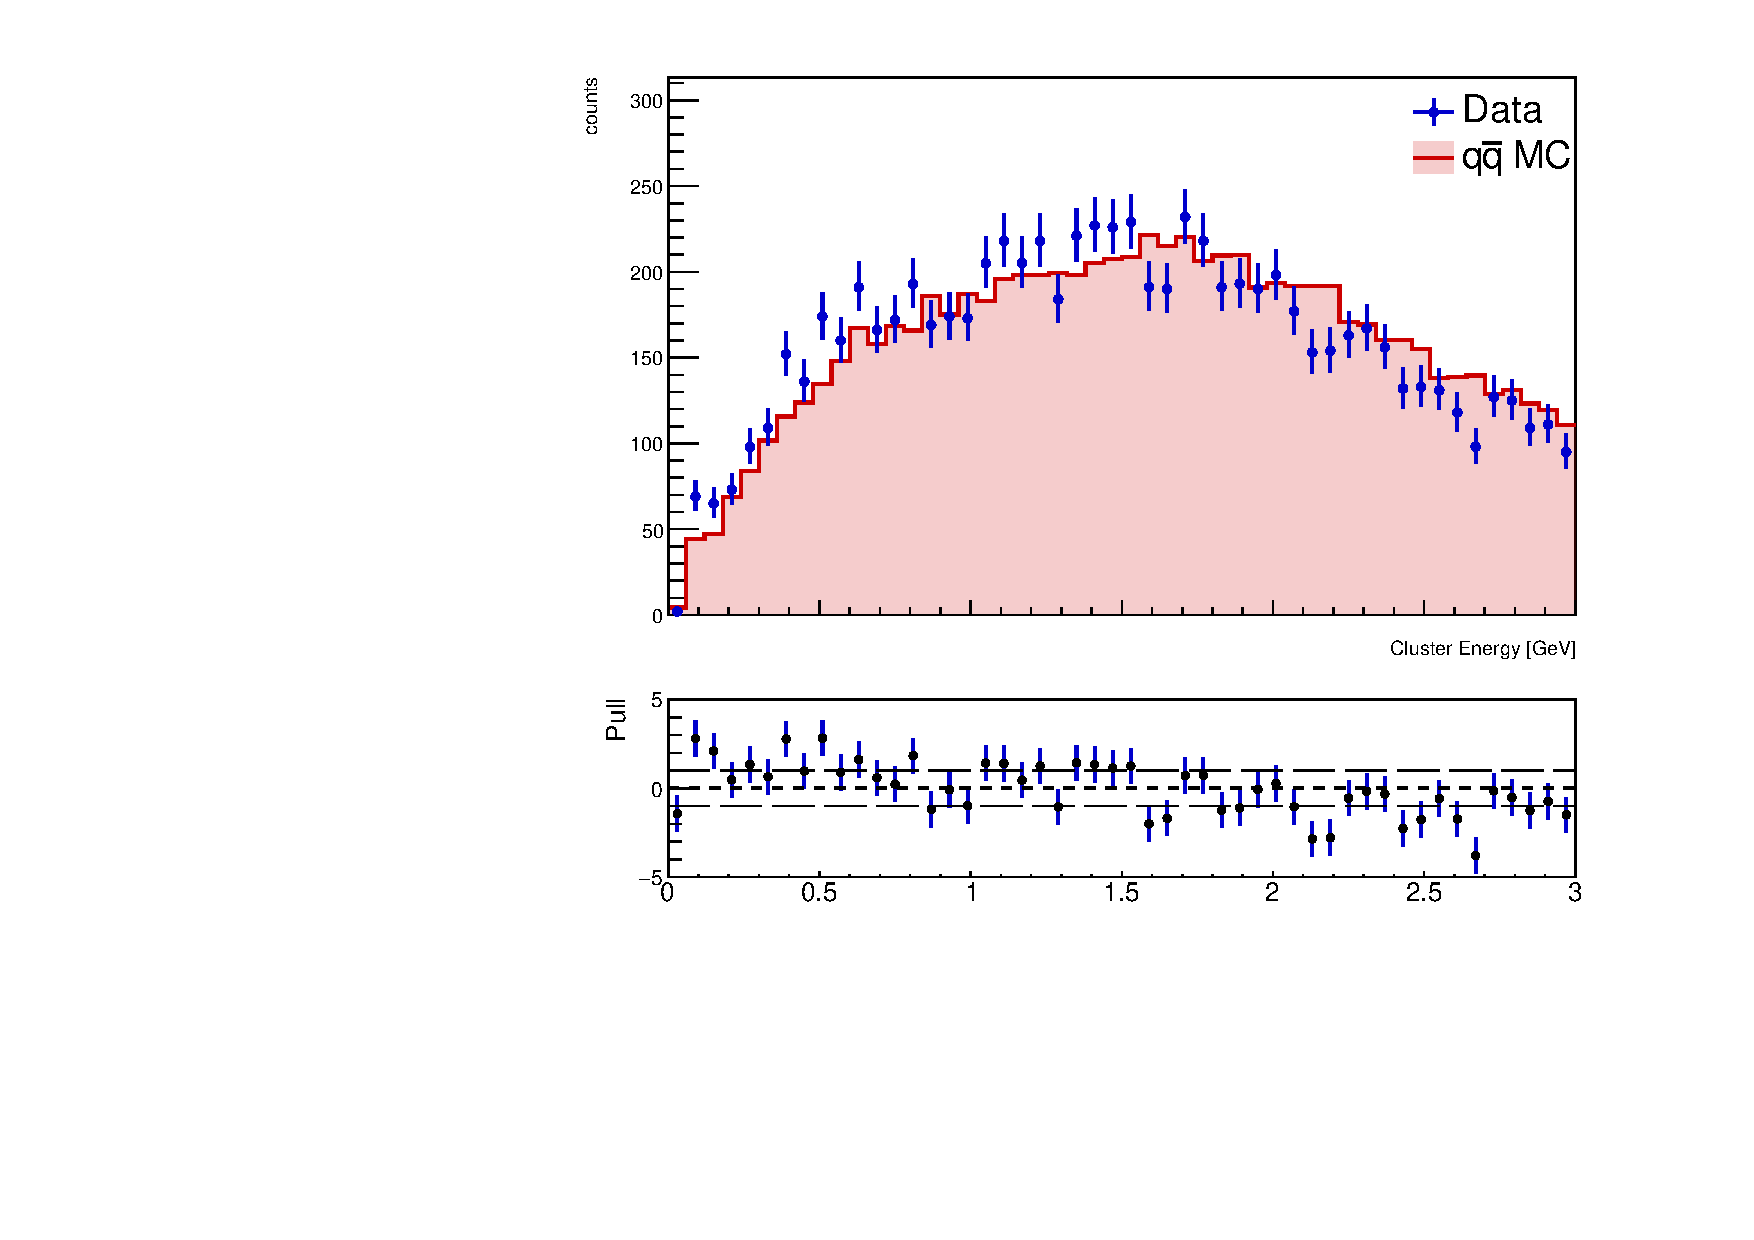
\includegraphics[width=0.49\textwidth]{nbar_data/images/dataMC_clusterE_isr_pull.pdf}
    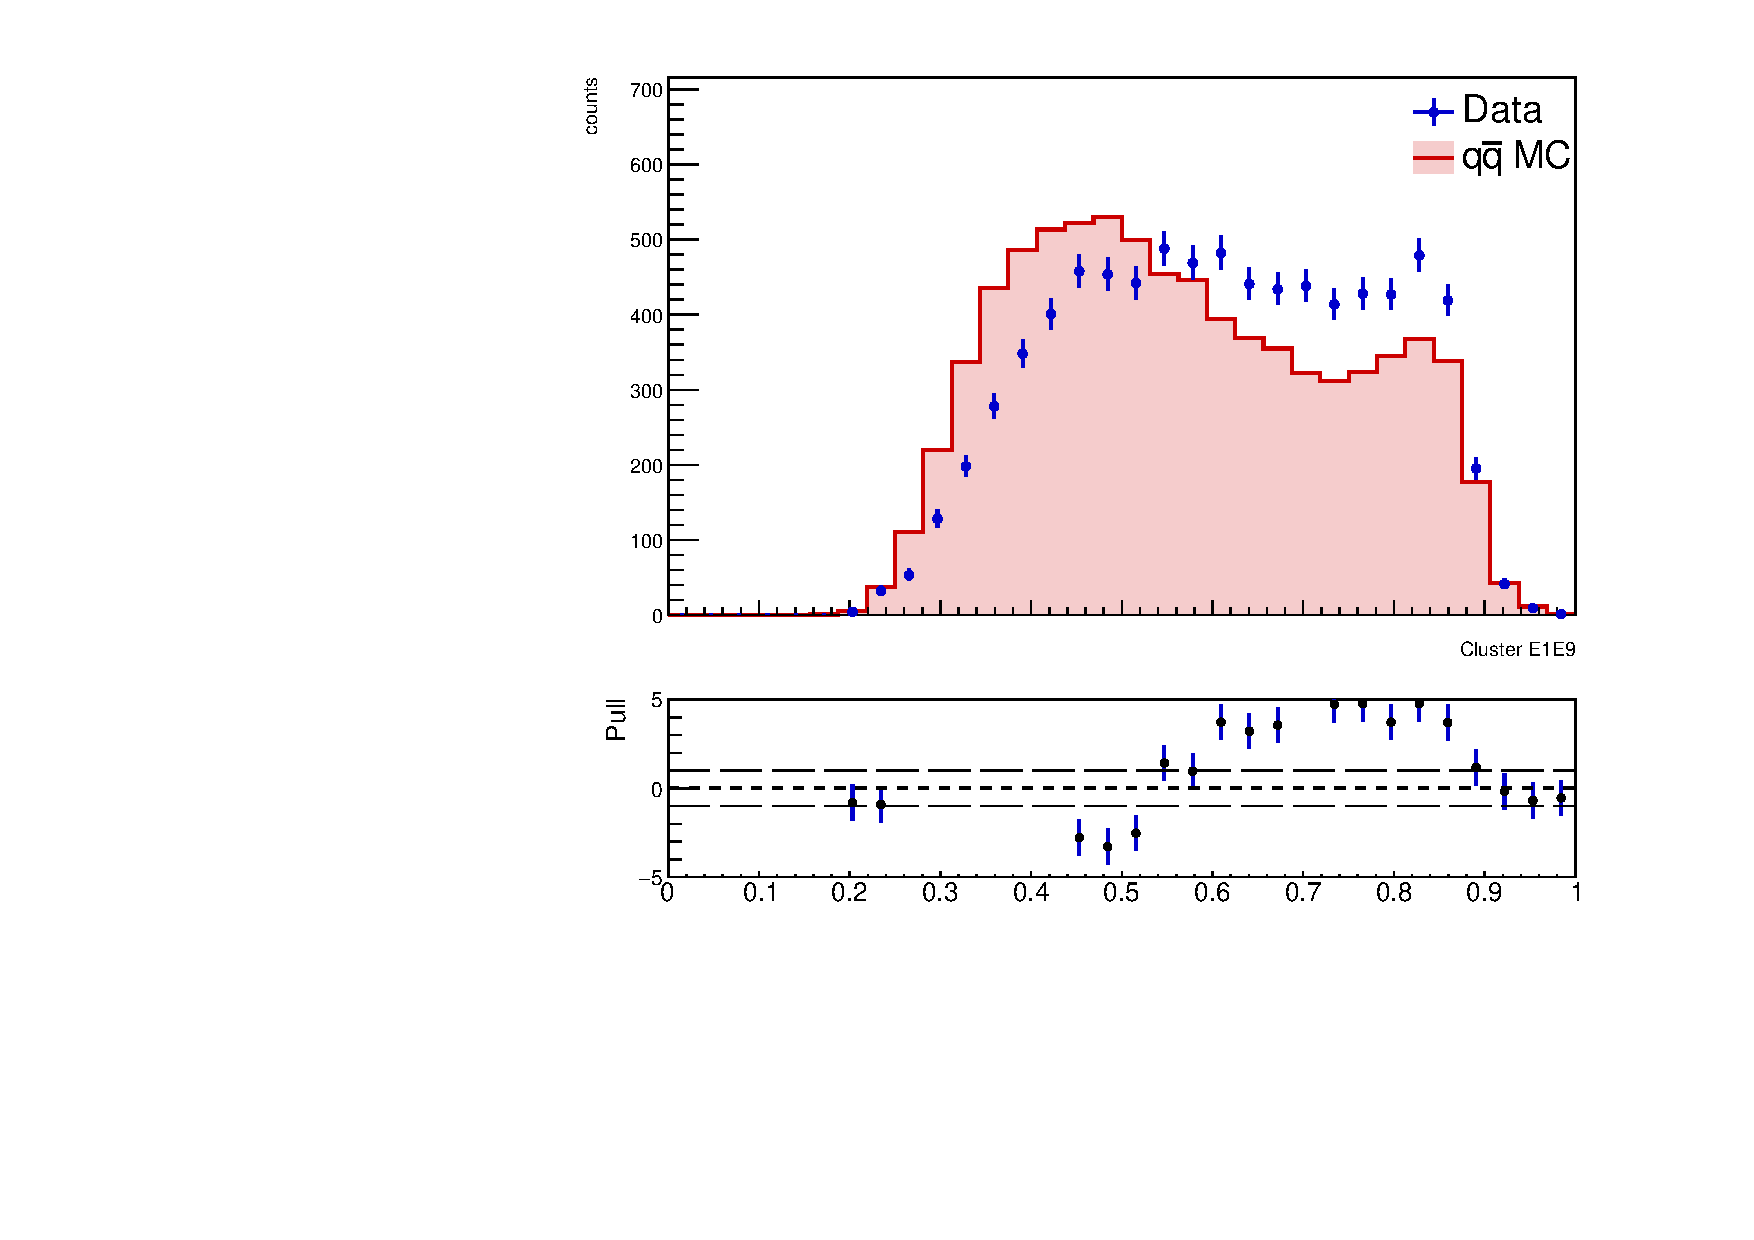
\includegraphics[width=0.49\textwidth]{nbar_data/images/dataMC_clusterE1E9_isr_pull.pdf}
    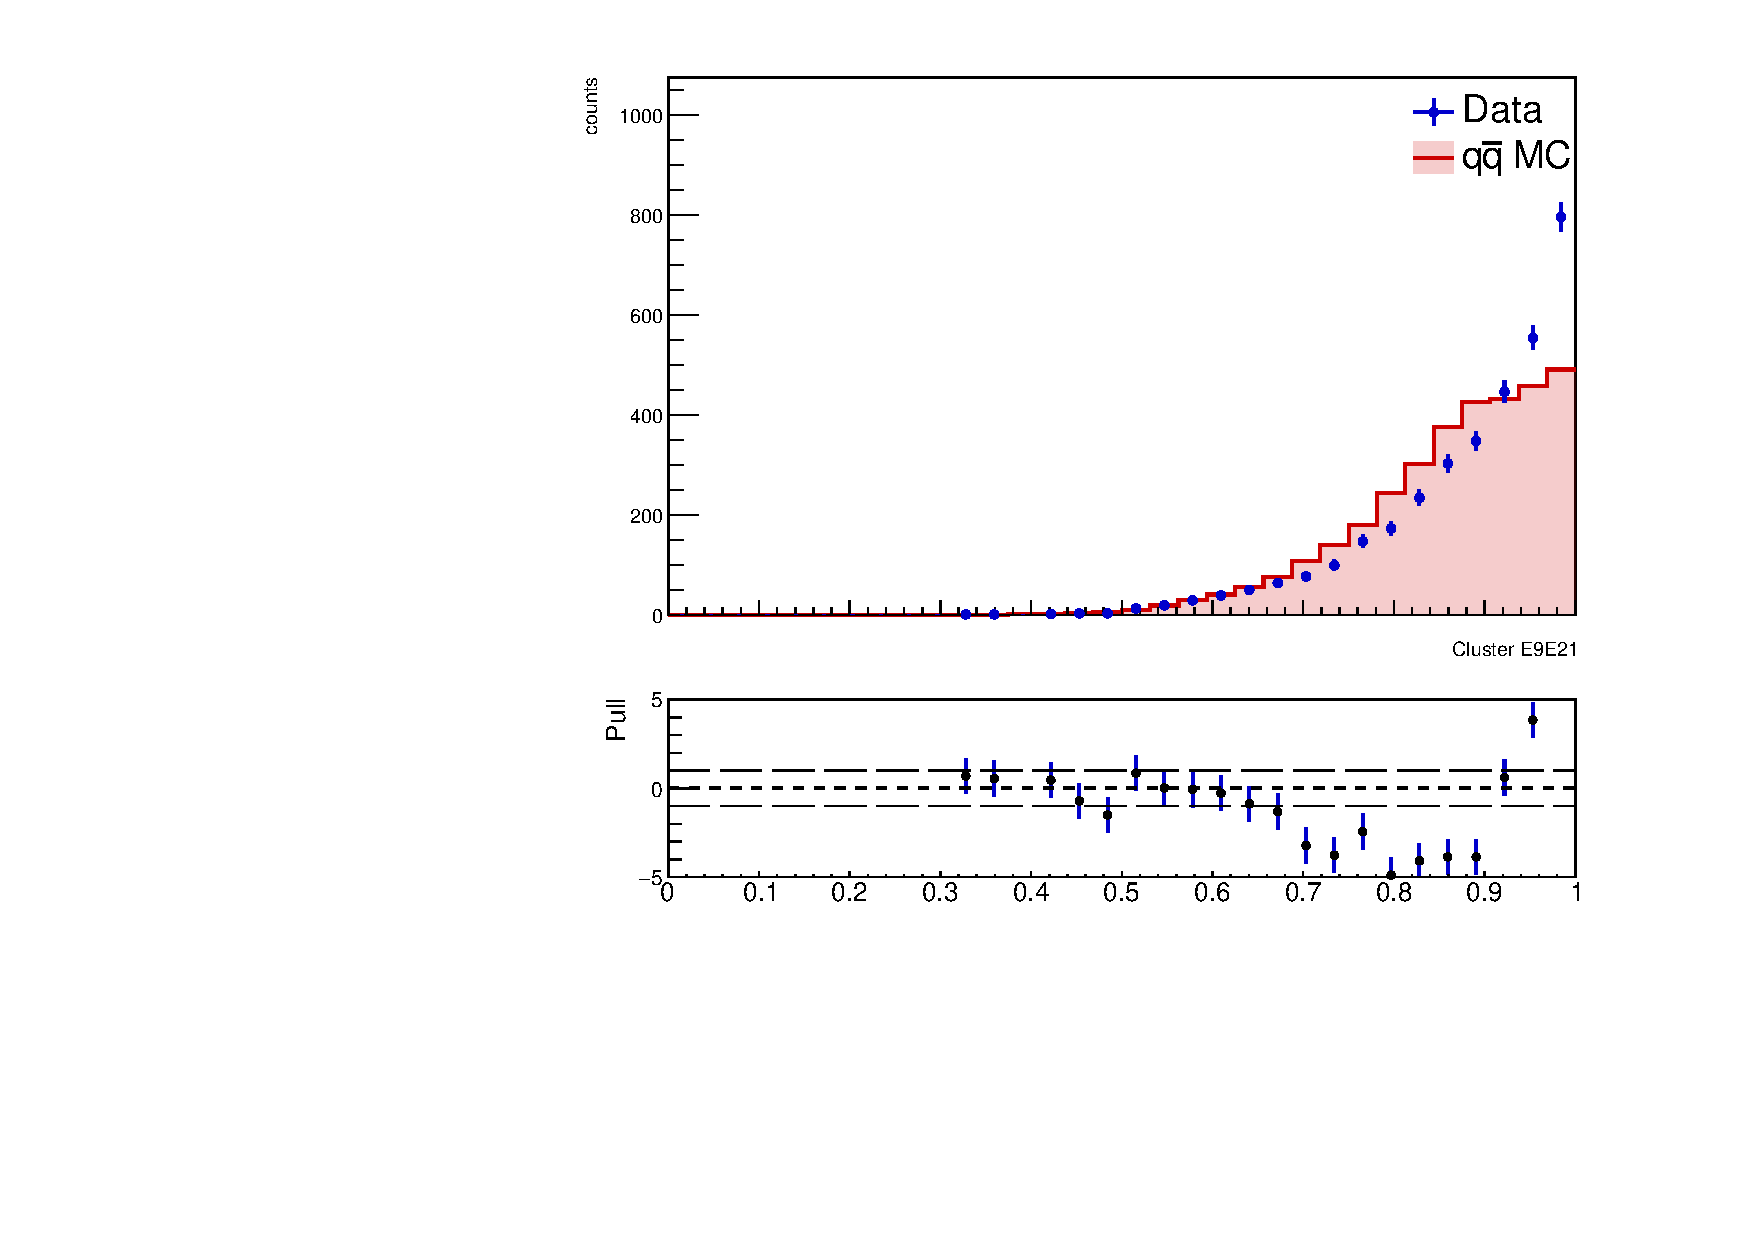
\includegraphics[width=0.49\textwidth]{nbar_data/images/dataMC_clusterE9E21_isr_pull.pdf}
    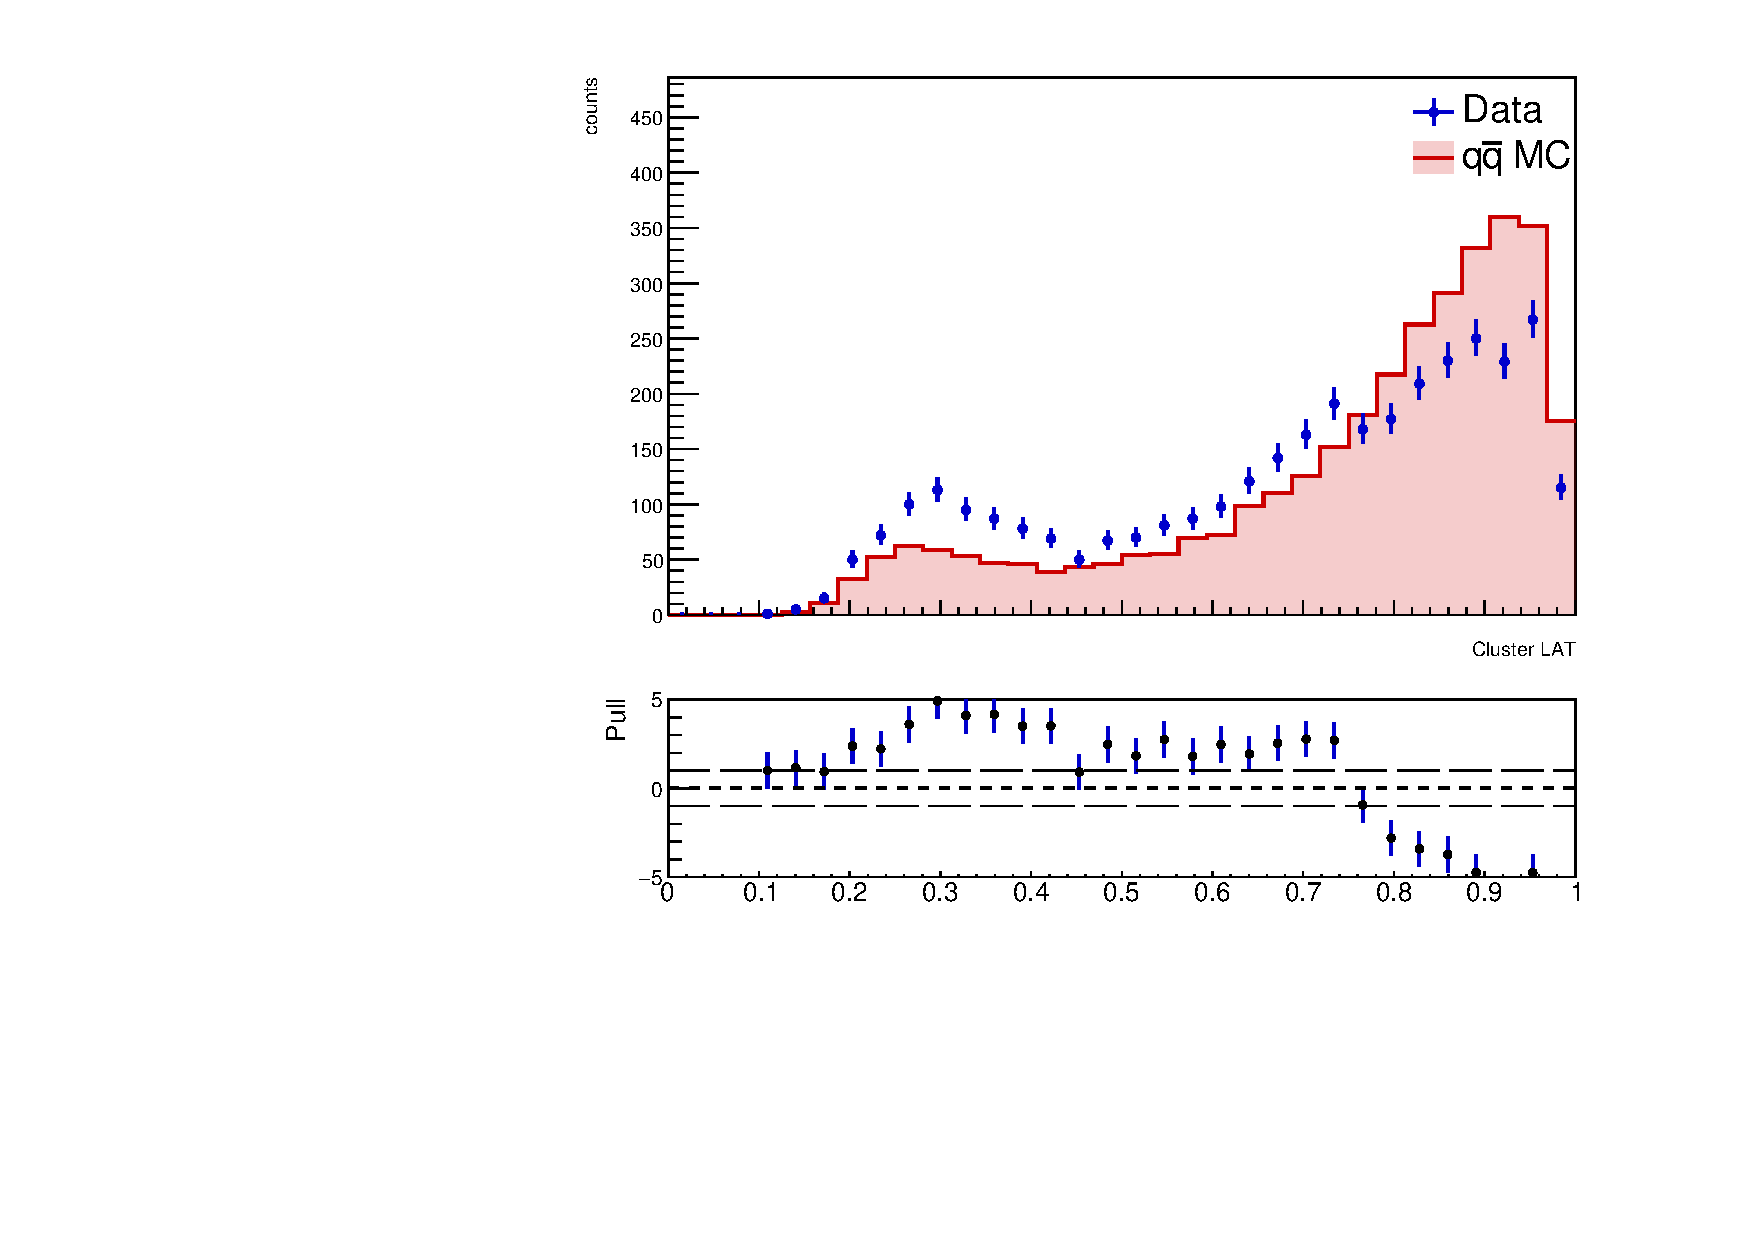
\includegraphics[width=0.49\textwidth]{nbar_data/images/dataMC_clusterLAT_isr_pull.pdf}
    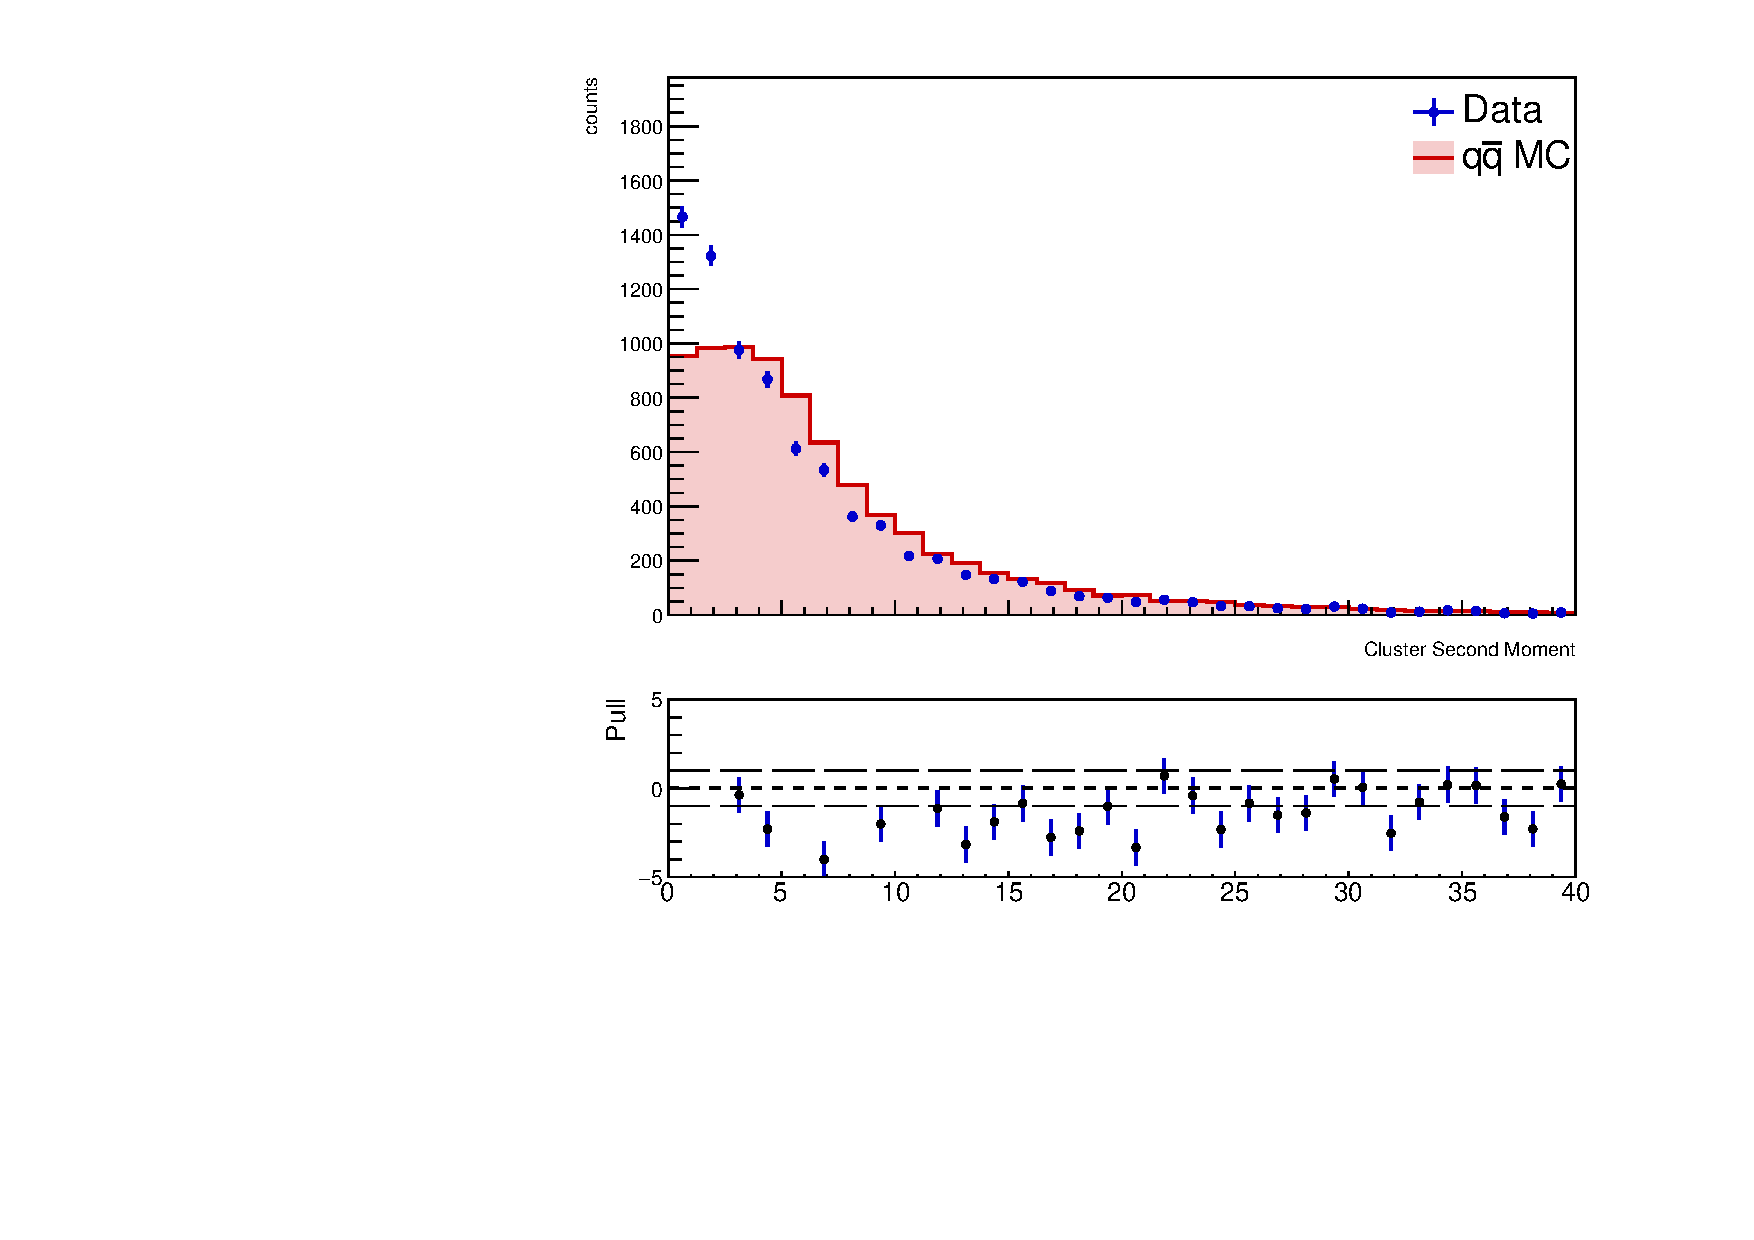
\includegraphics[width=0.49\textwidth]{nbar_data/images/dataMC_clusterSecondMoment_isr_pull.pdf}
    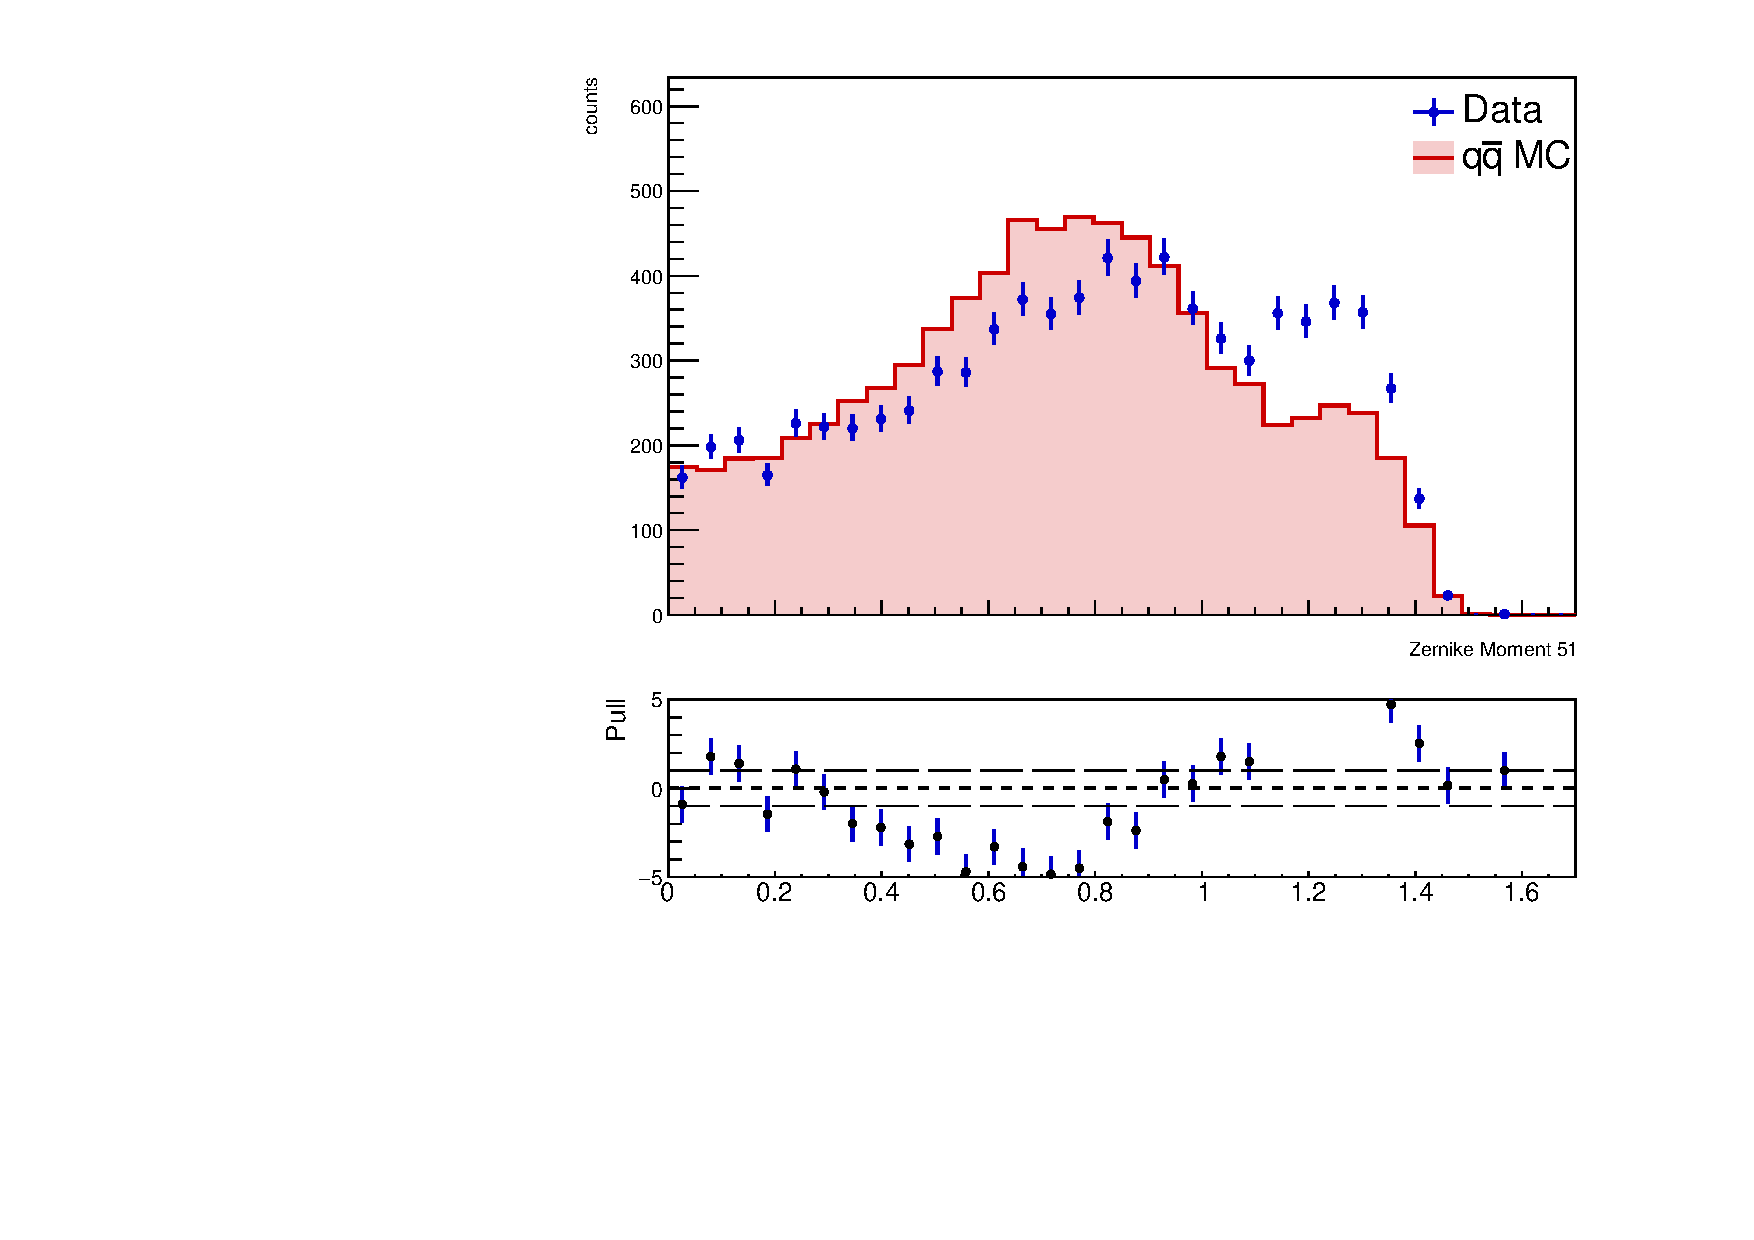
\includegraphics[width=0.49\textwidth]{nbar_data/images/dataMC_clusterAbsZernikeMoment40_isr_pull.pdf}
    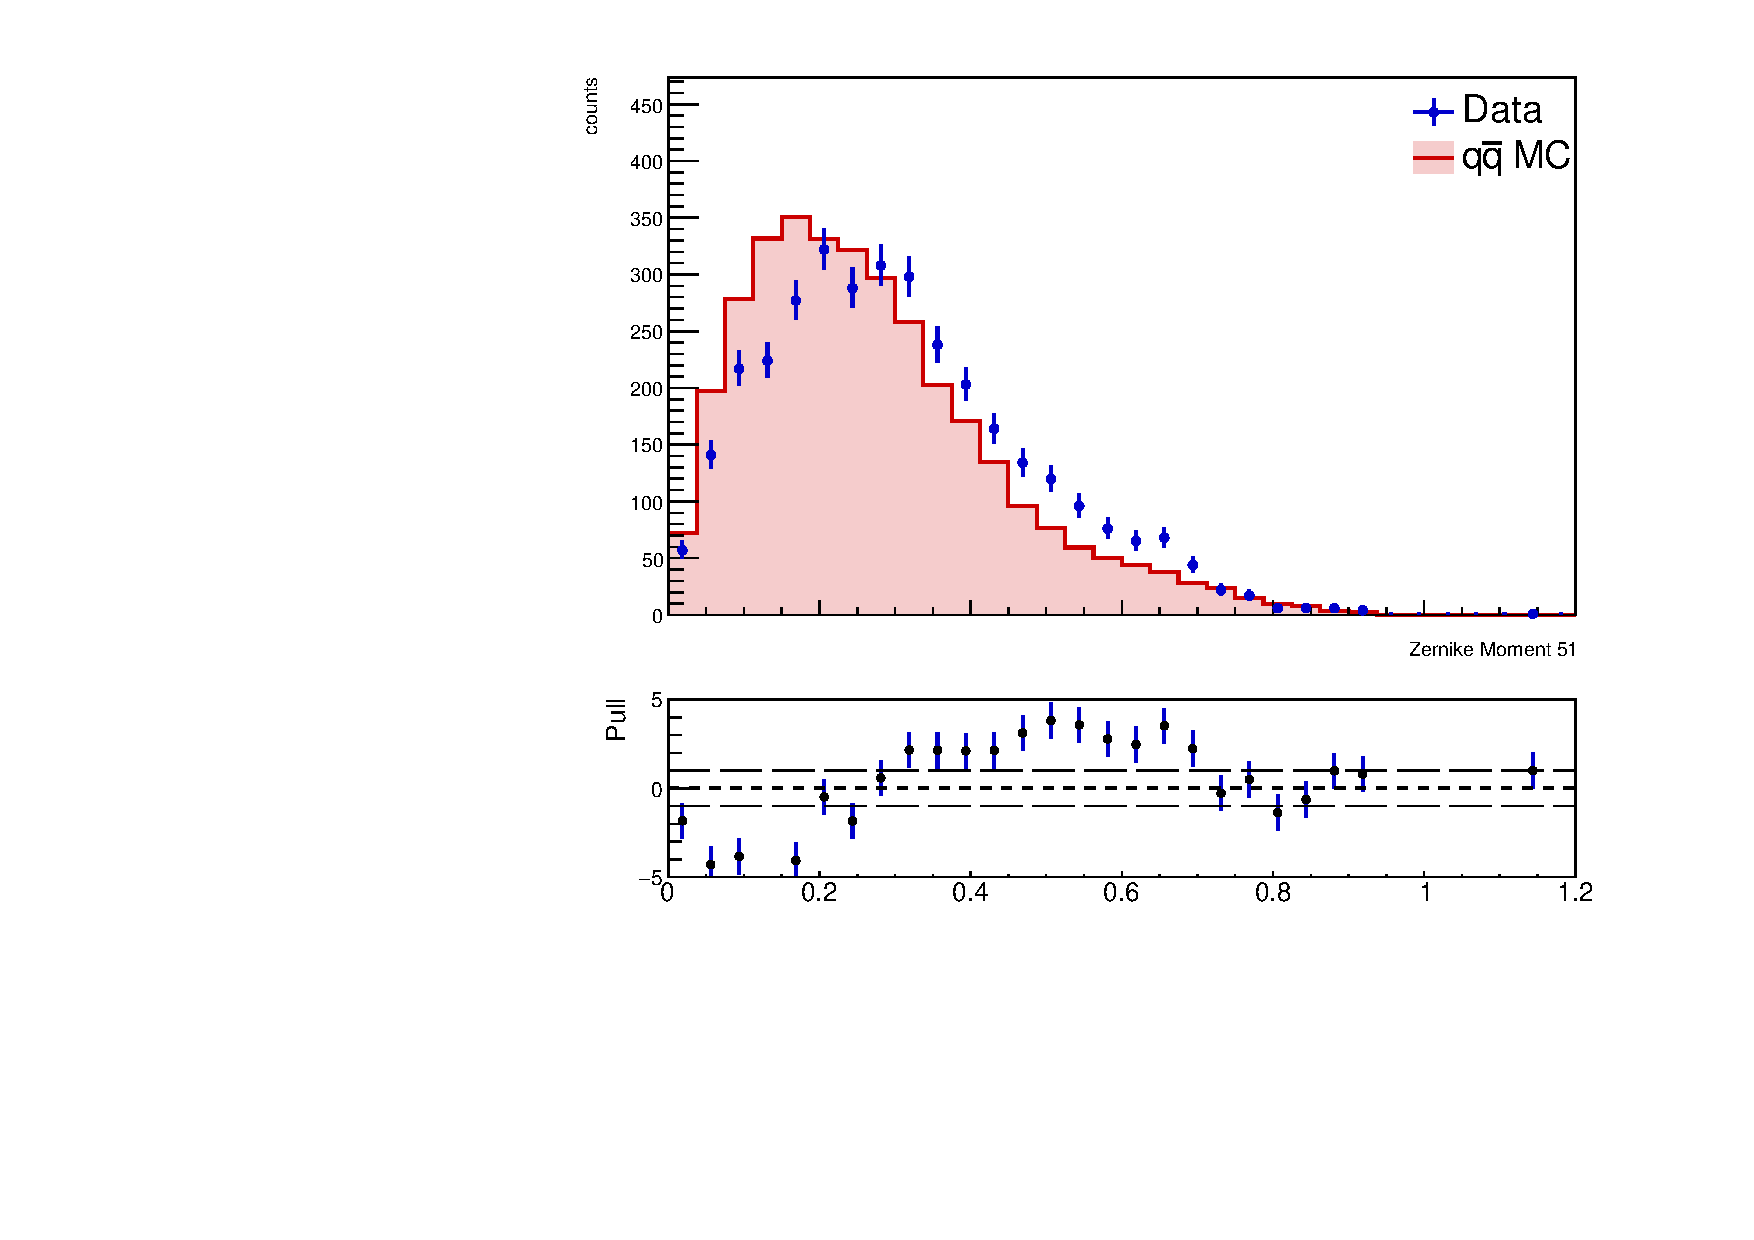
\includegraphics[width=0.49\textwidth]{nbar_data/images/dataMC_clusterAbsZernikeMoment51_isr_pull.pdf}
    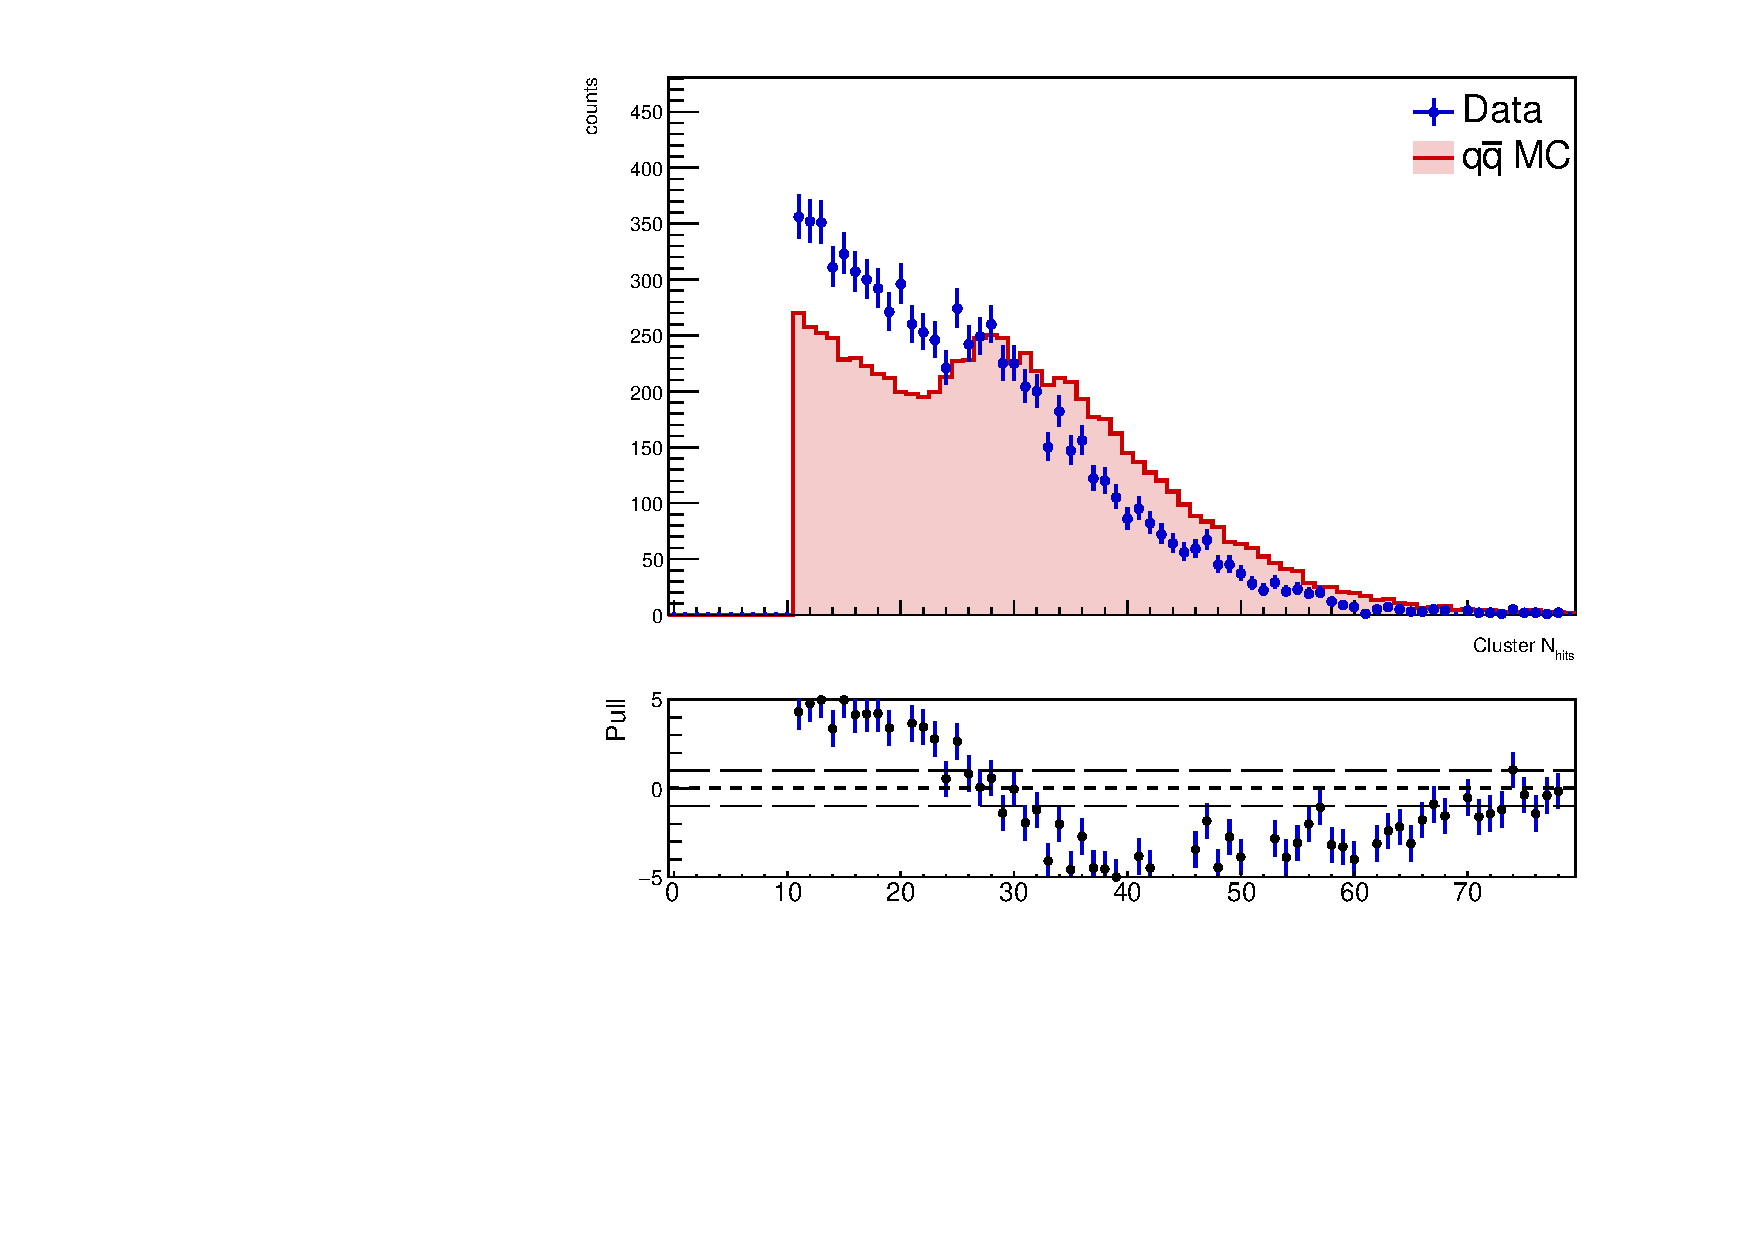
\includegraphics[width=0.49\textwidth]{nbar_data/images/dataMC_clusterNHits_isr_pull.pdf}
   
     \caption{Data/MC agreement for reconstructed cluster variables for $\bar{n}$ candidates, in ISR case.}
     \label{fig:dataMC_isr_nosid}
\end{figure}

 \begin{figure}[H]
    \centering
    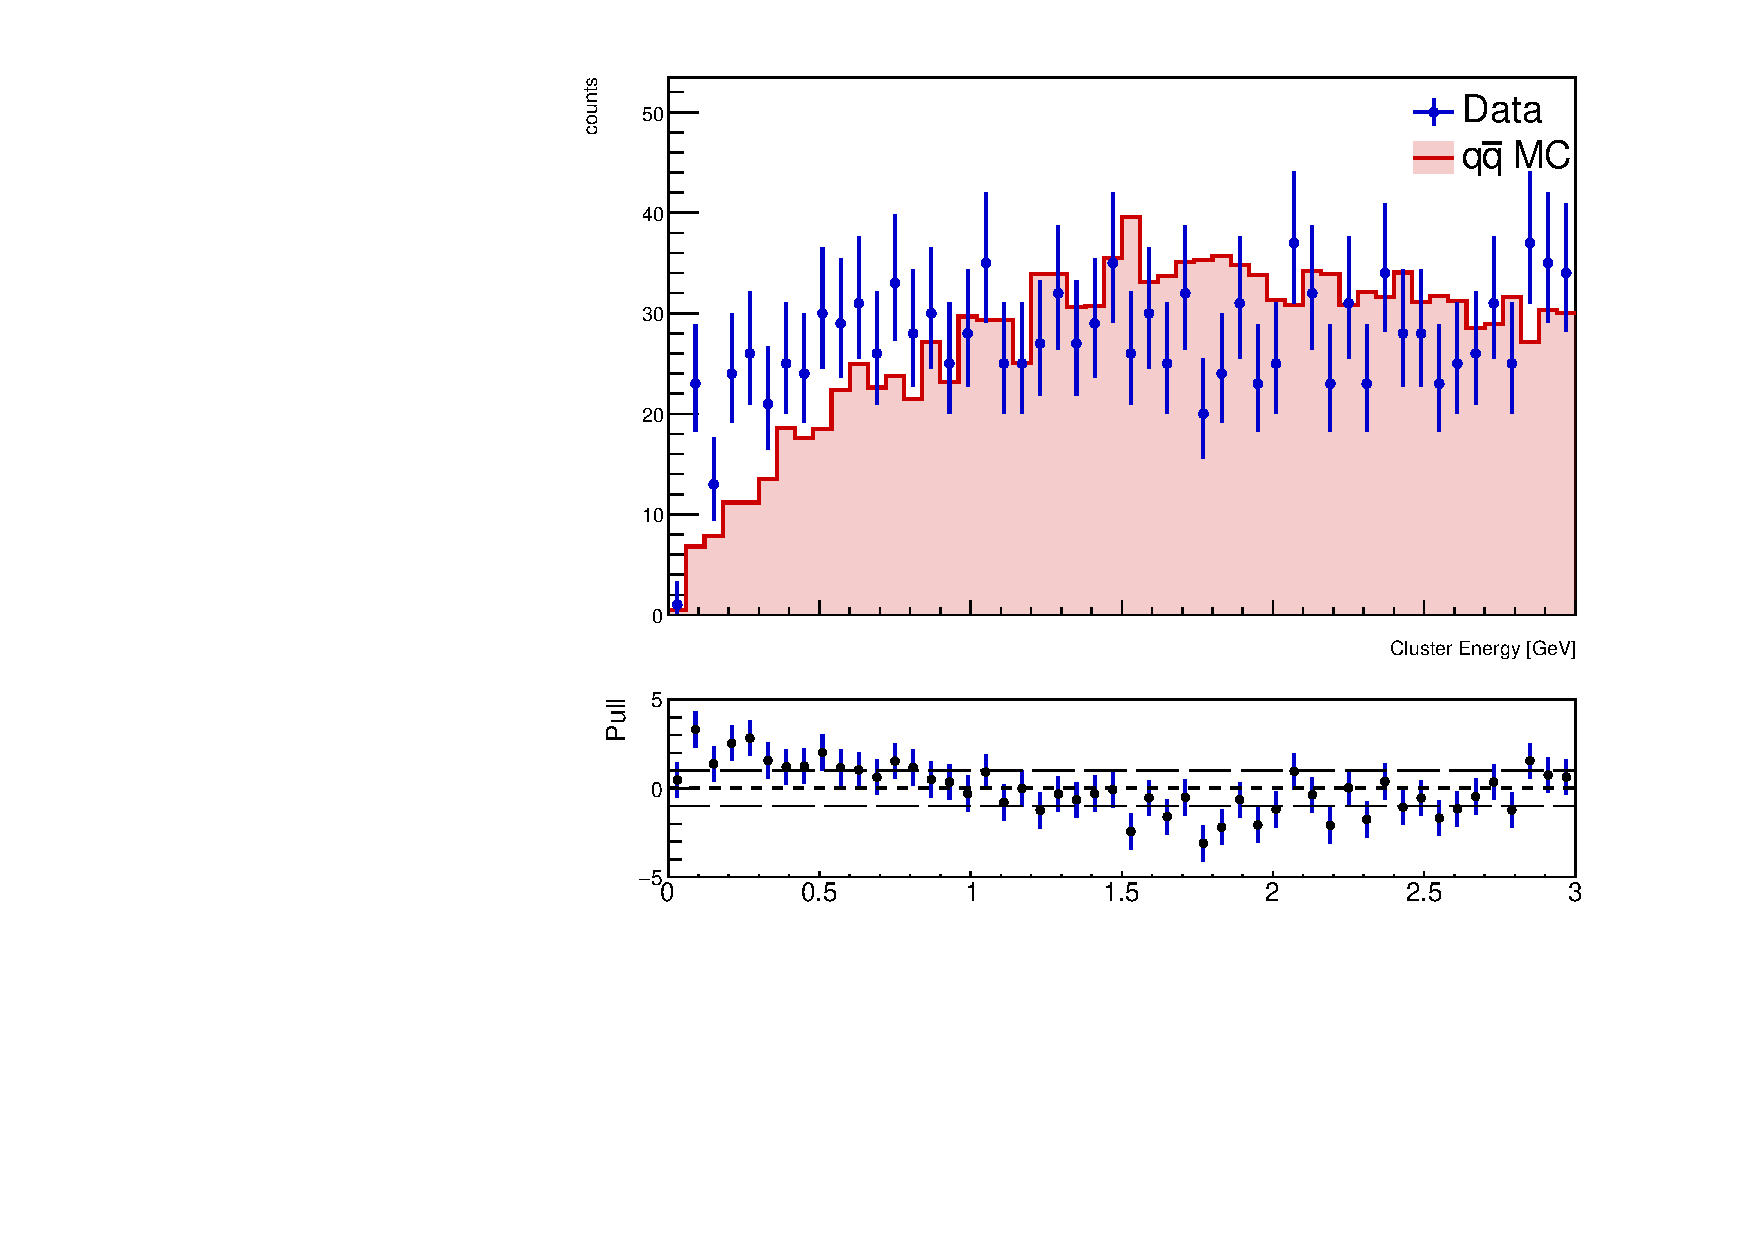
\includegraphics[width=0.49\textwidth]{nbar_data/images/dataMC_clusterE_nog_pull.pdf}
    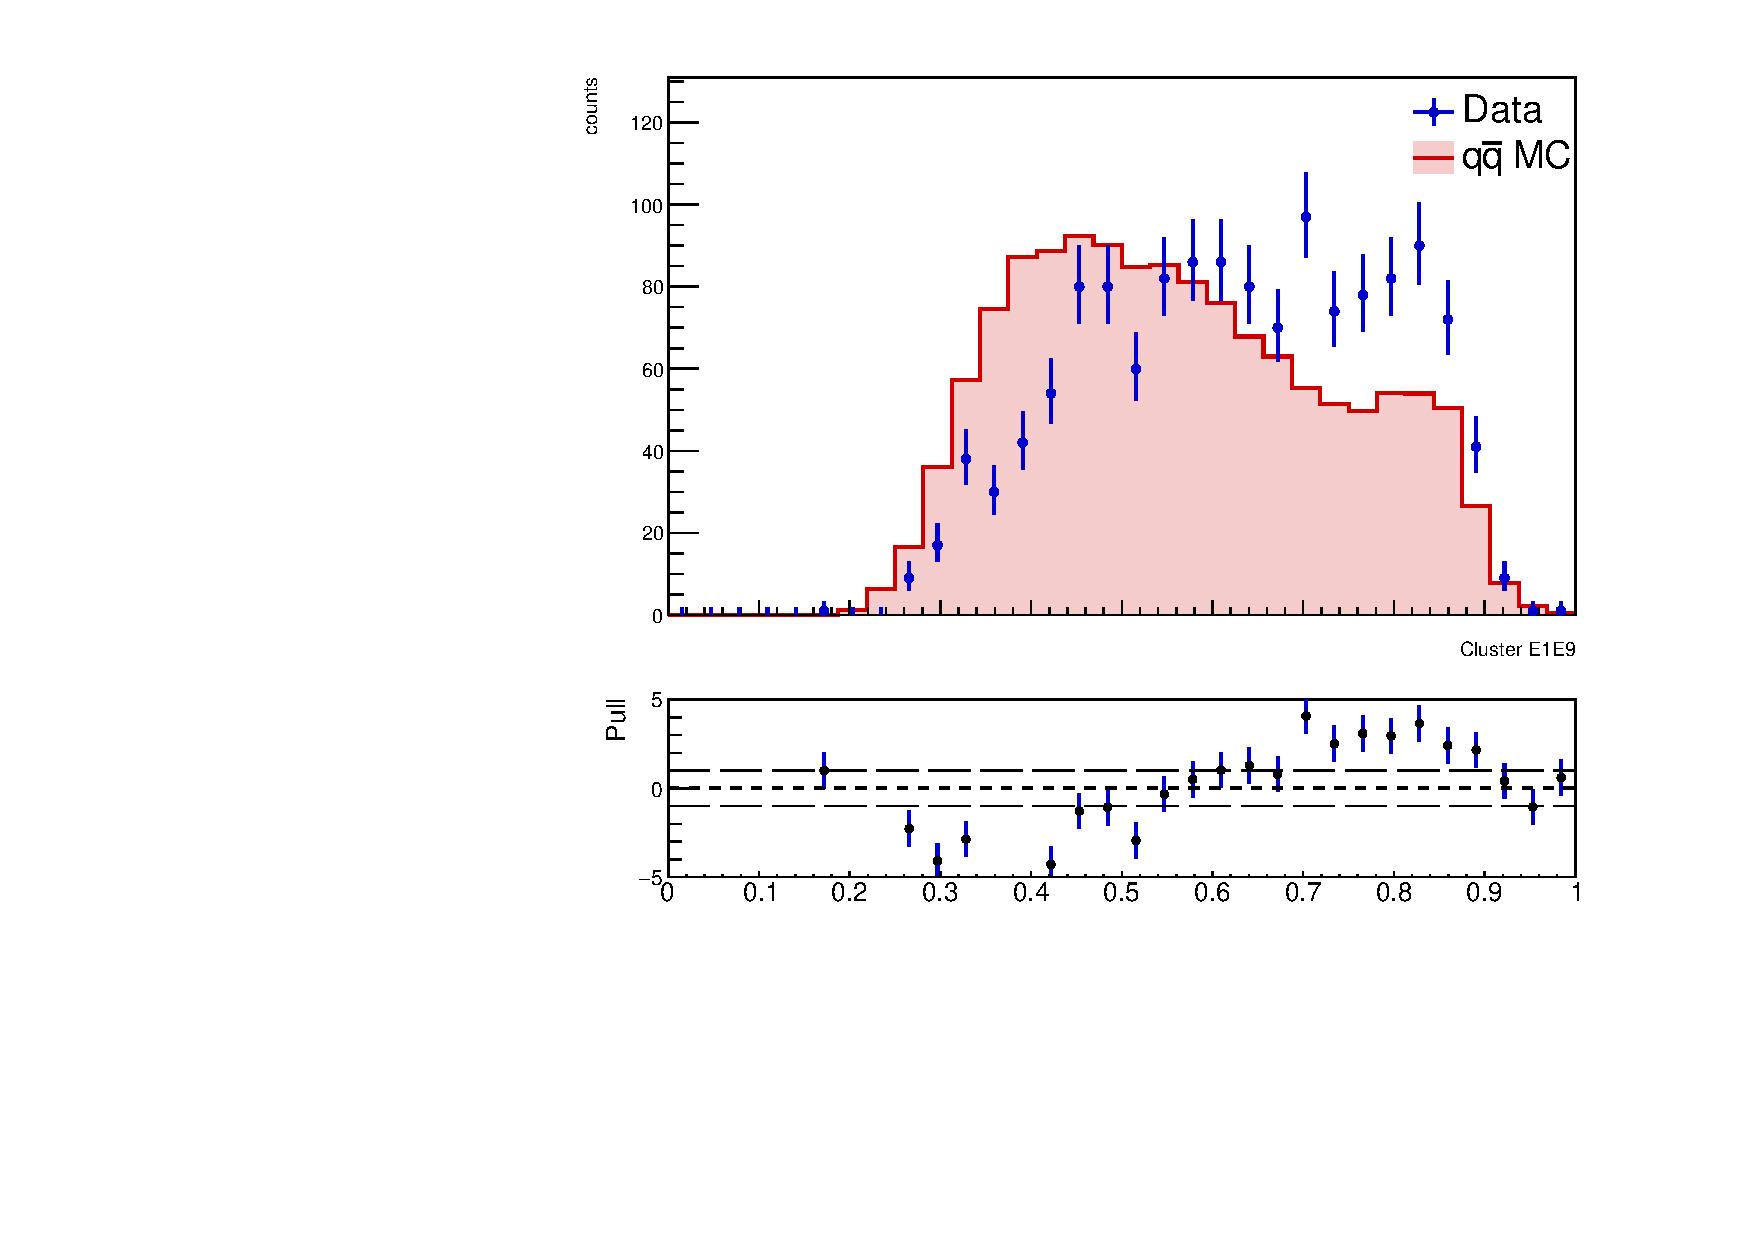
\includegraphics[width=0.49\textwidth]{nbar_data/images/dataMC_clusterE1E9_nog_pull.pdf}
    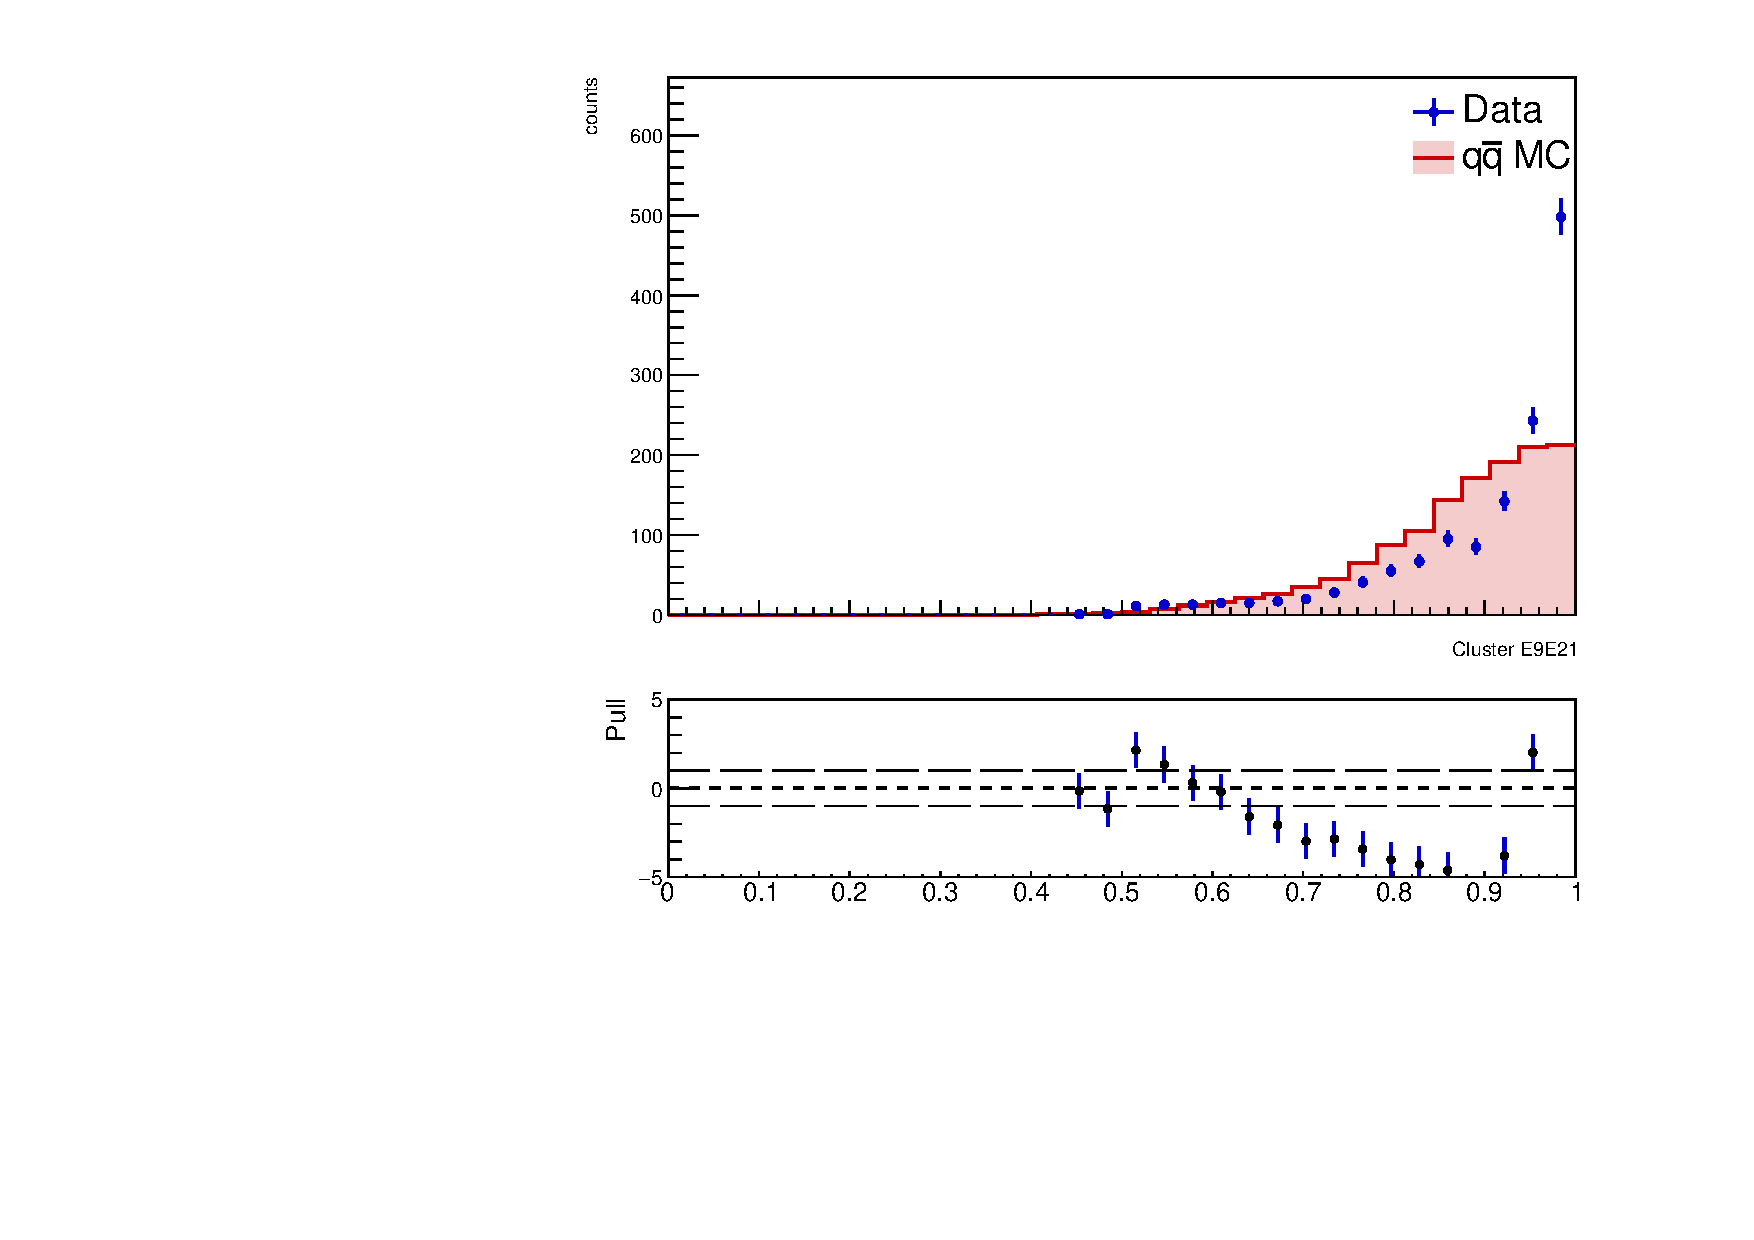
\includegraphics[width=0.49\textwidth]{nbar_data/images/dataMC_clusterE9E21_nog_pull.pdf}
    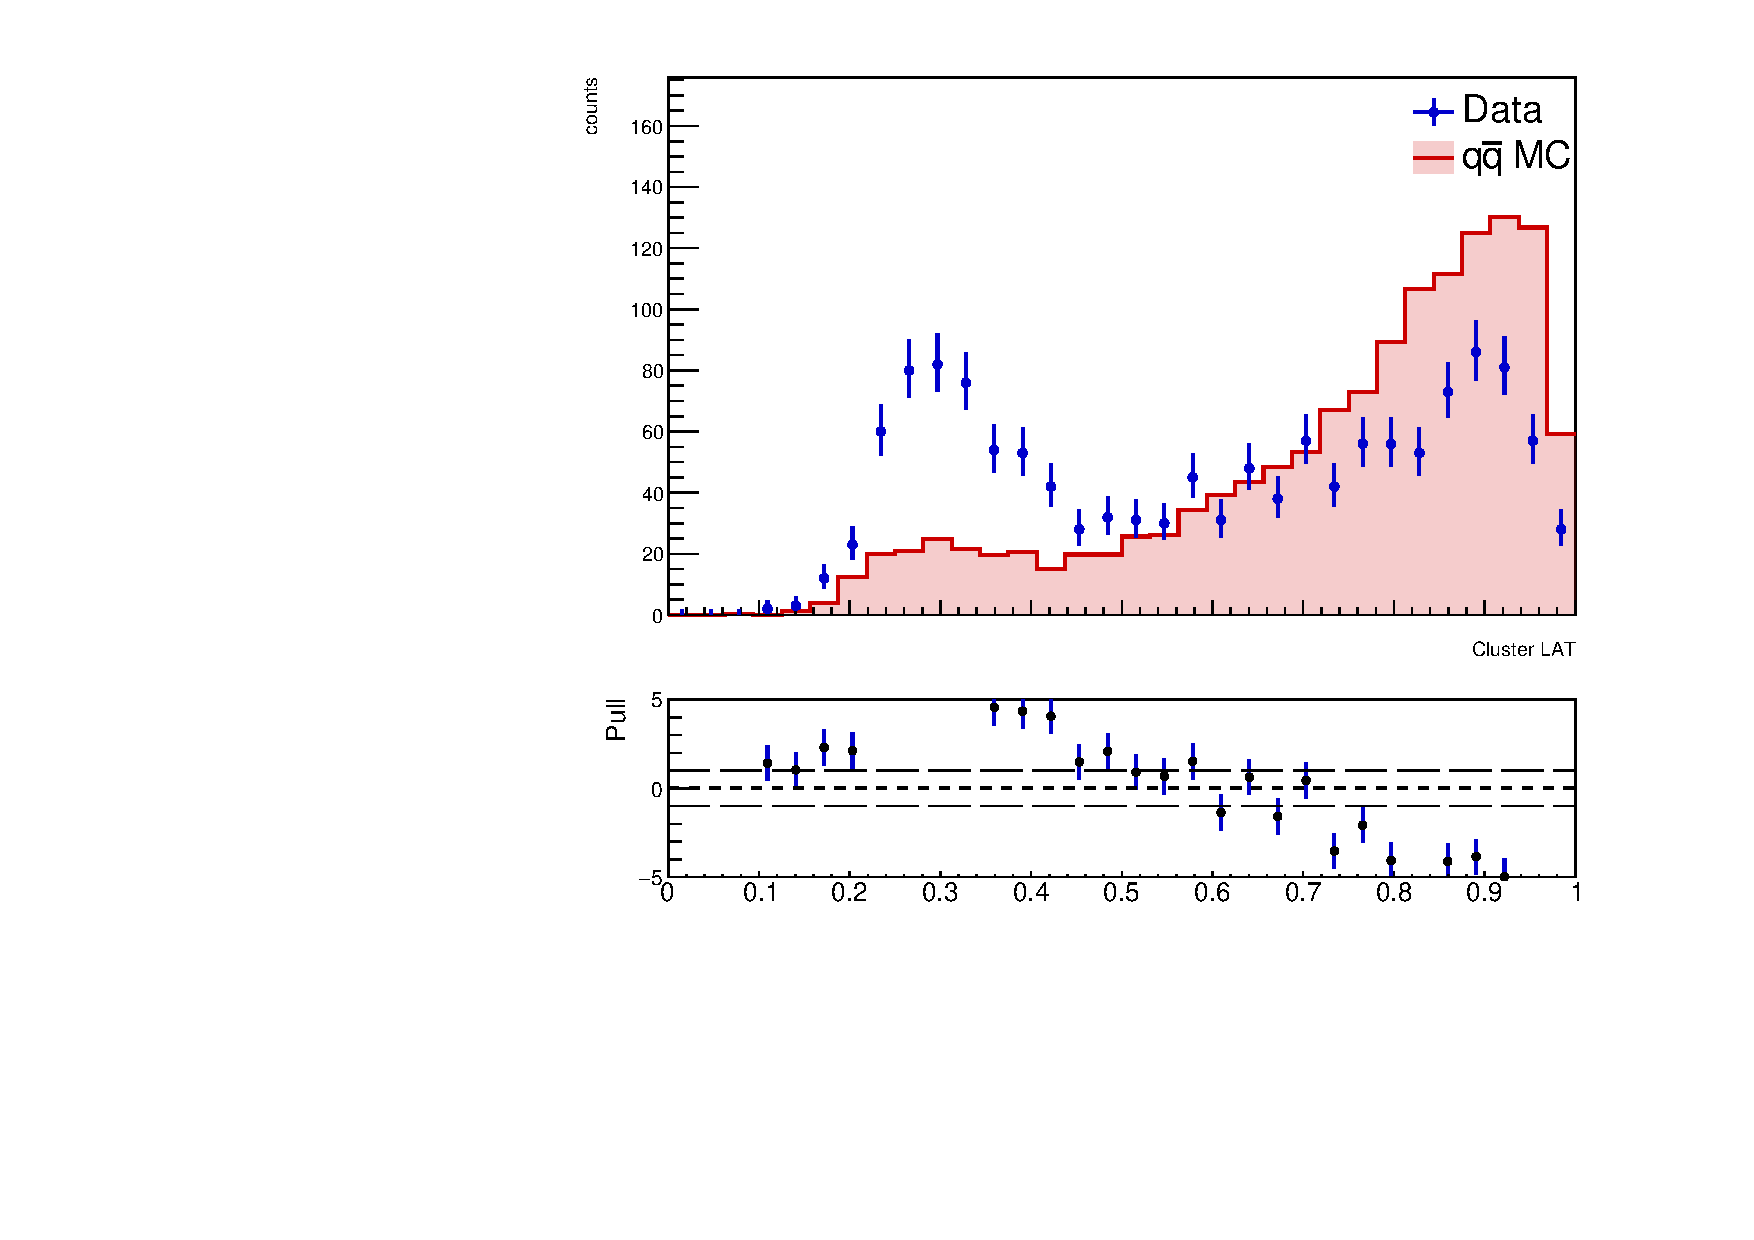
\includegraphics[width=0.49\textwidth]{nbar_data/images/dataMC_clusterLAT_nog_pull.pdf}
    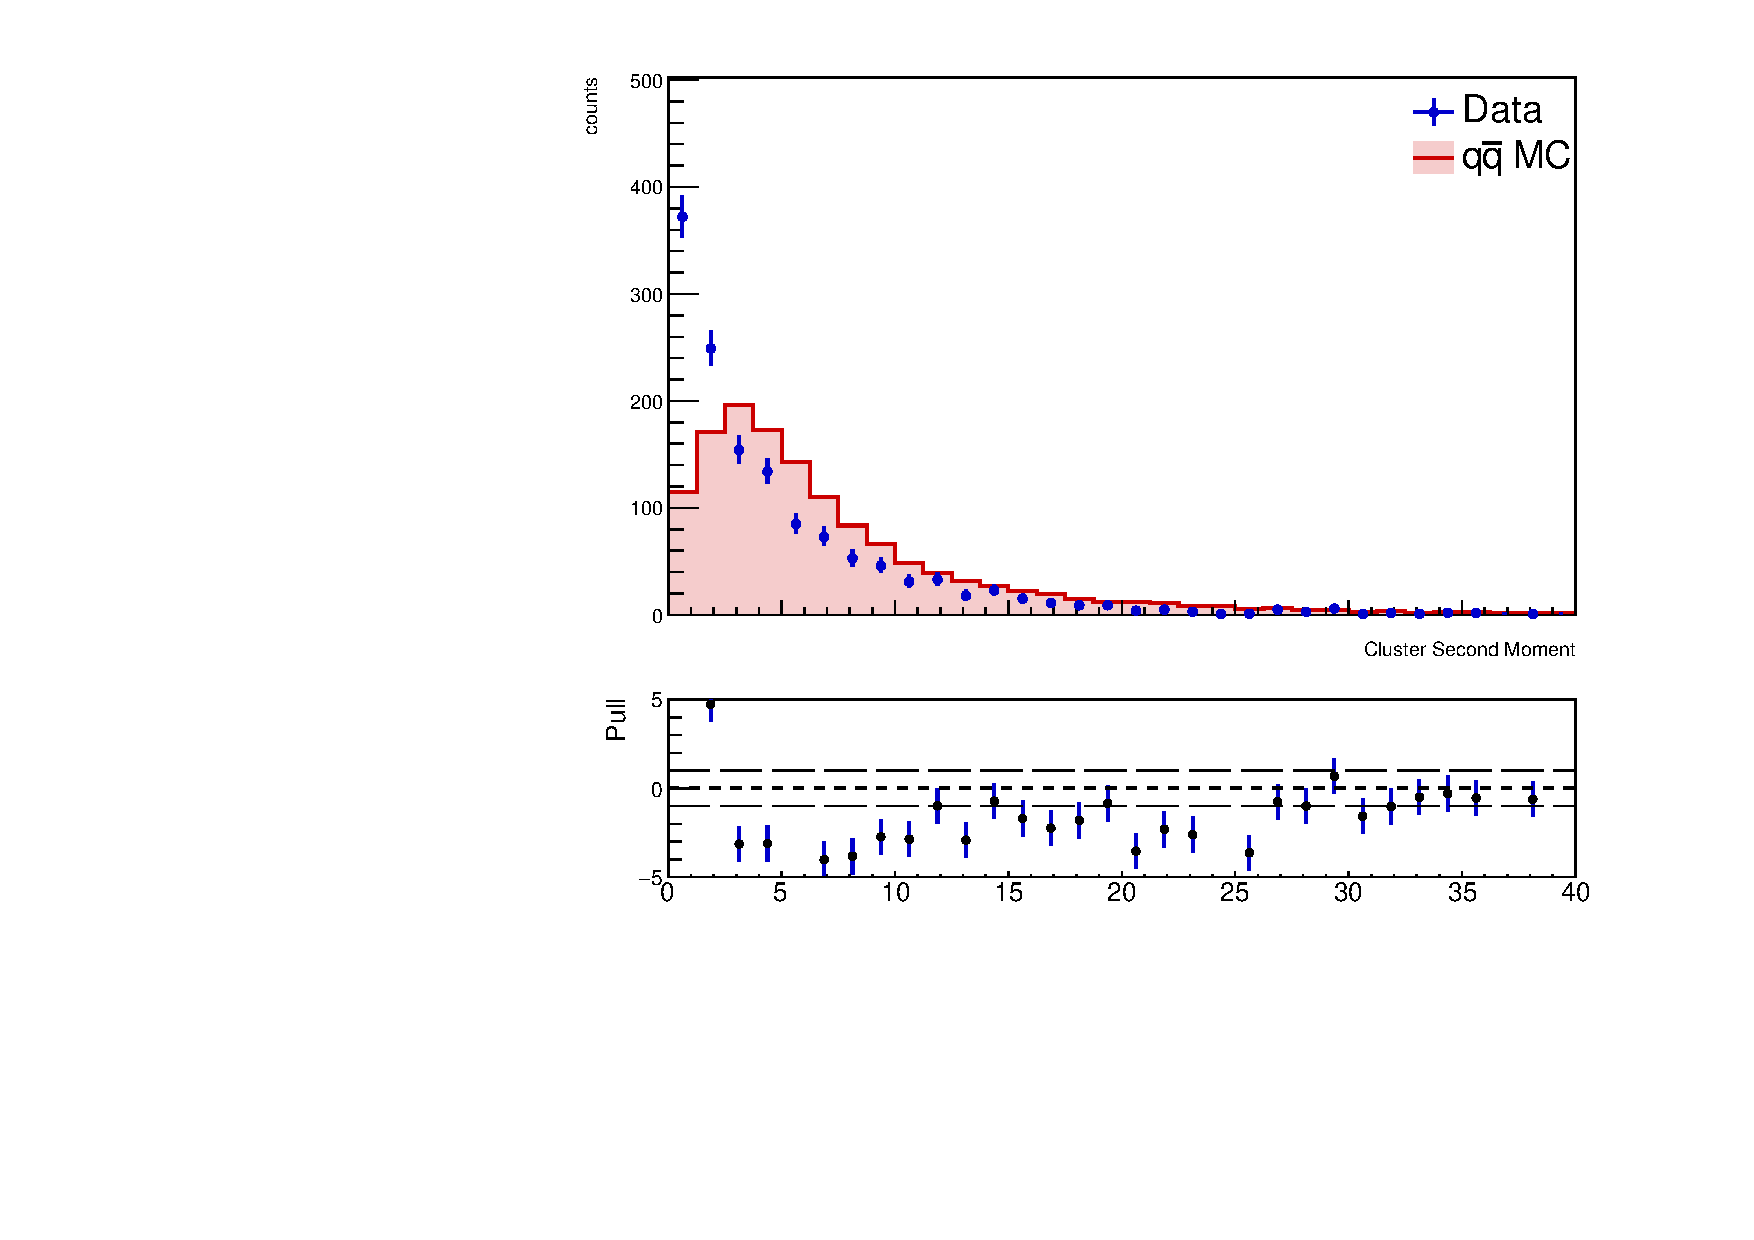
\includegraphics[width=0.49\textwidth]{nbar_data/images/dataMC_clusterSecondMoment_nog_pull.pdf}
    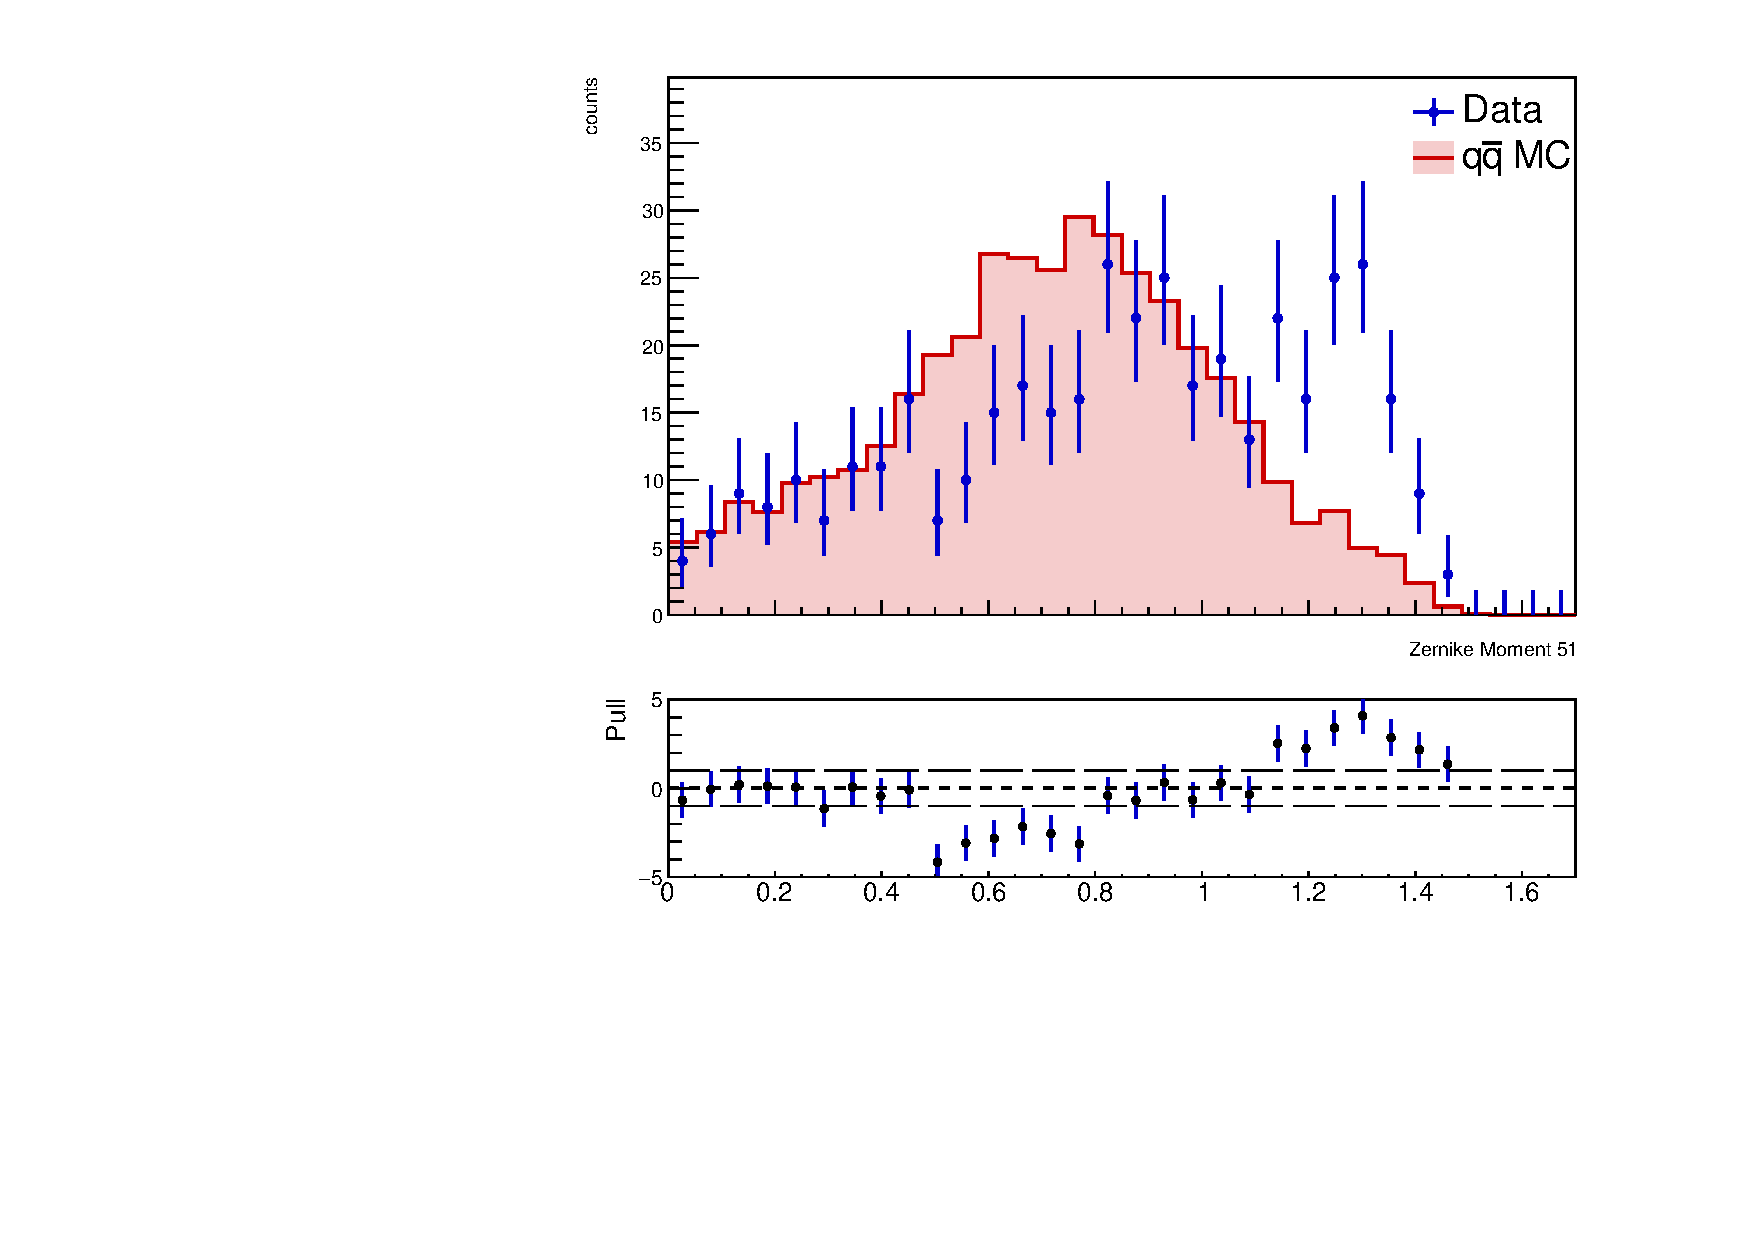
\includegraphics[width=0.49\textwidth]{nbar_data/images/dataMC_clusterAbsZernikeMoment40_nog_pull.pdf}
    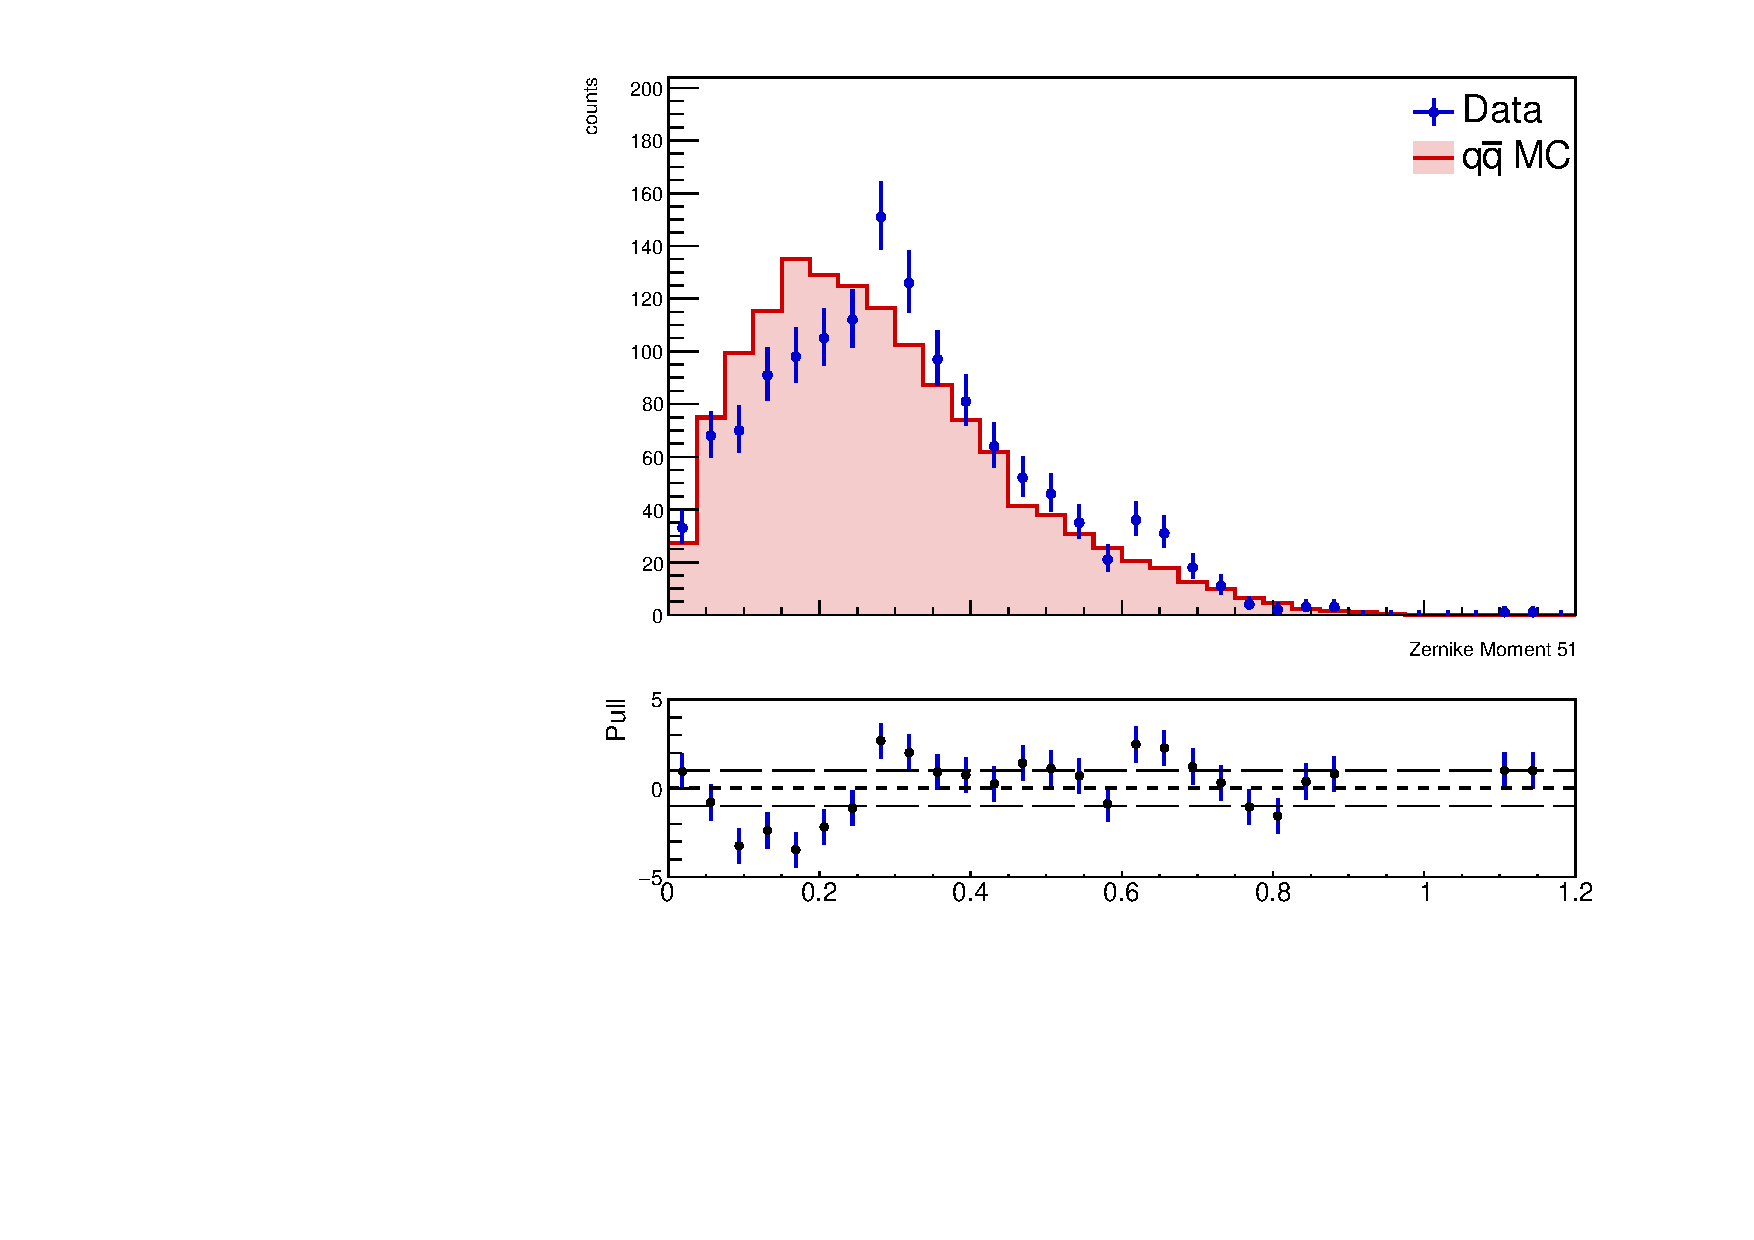
\includegraphics[width=0.49\textwidth]{nbar_data/images/dataMC_clusterAbsZernikeMoment51_nog_pull.pdf}
    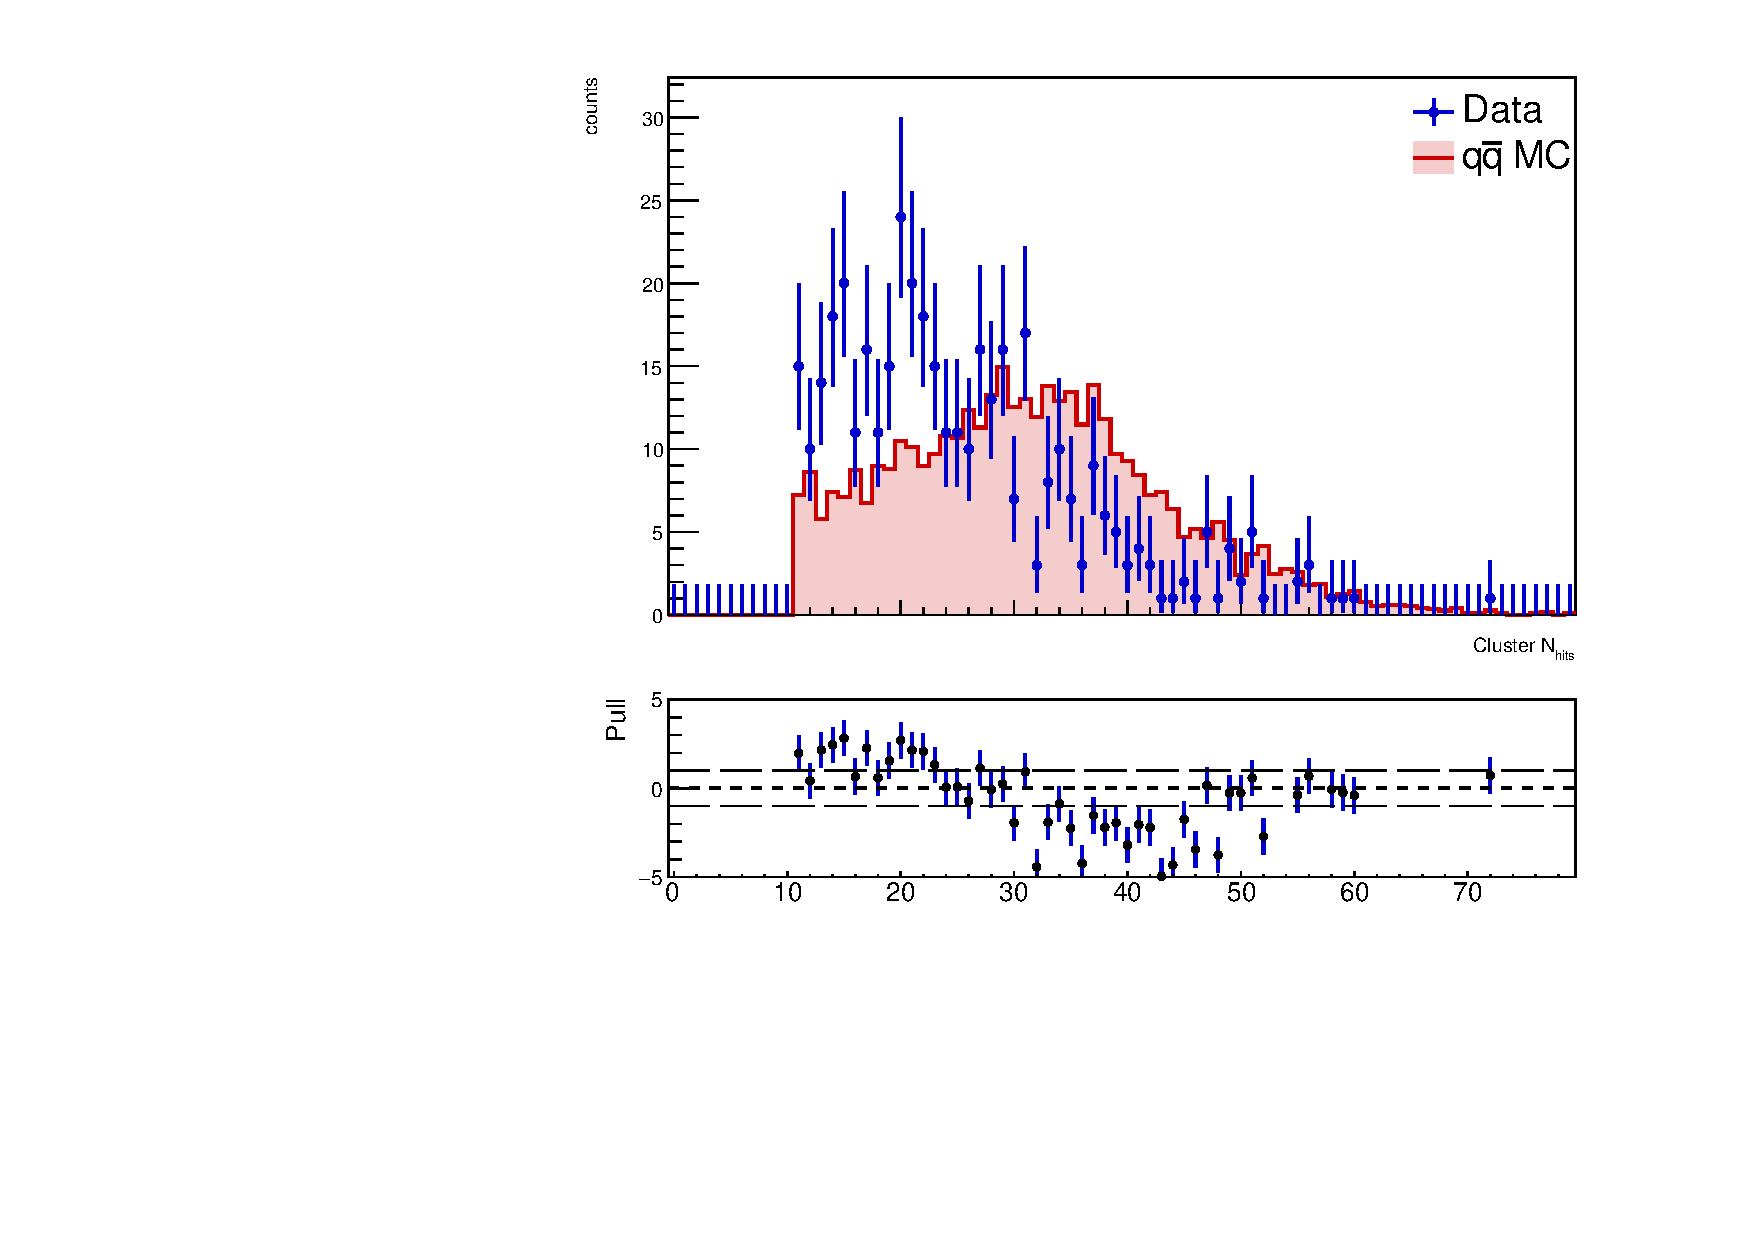
\includegraphics[width=0.49\textwidth]{nbar_data/images/dataMC_clusterNHits_nog_pull.pdf}
   
     \caption{Data/MC agreement for reconstructed cluster variables for $\bar{n}$ candidates, in NO ISR case.}
     \label{fig:dataMC_nog_nosid}
\end{figure}

 \begin{figure}[H]
    \centering
    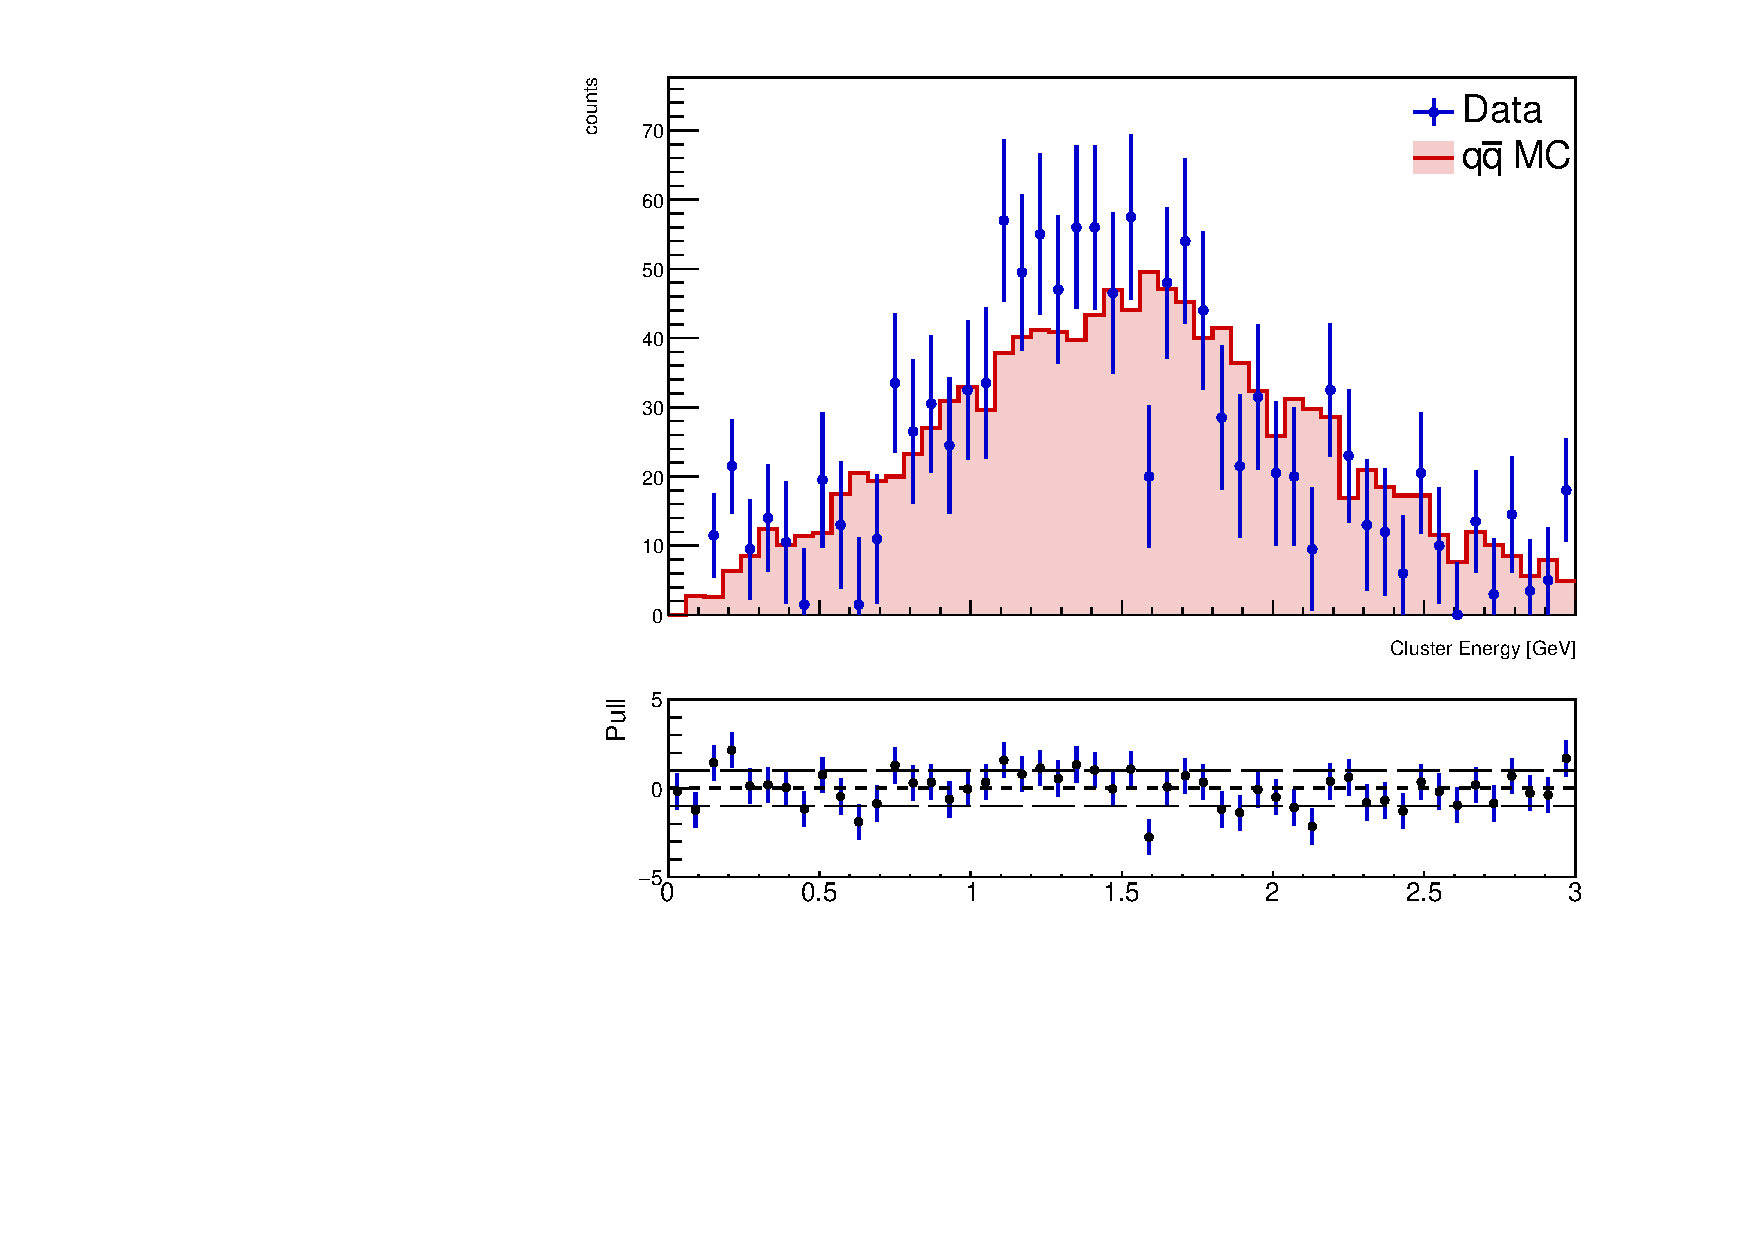
\includegraphics[width=0.49\textwidth]{nbar_data/images/dataMC_clusterE_isr_pull_subtracted.pdf}
    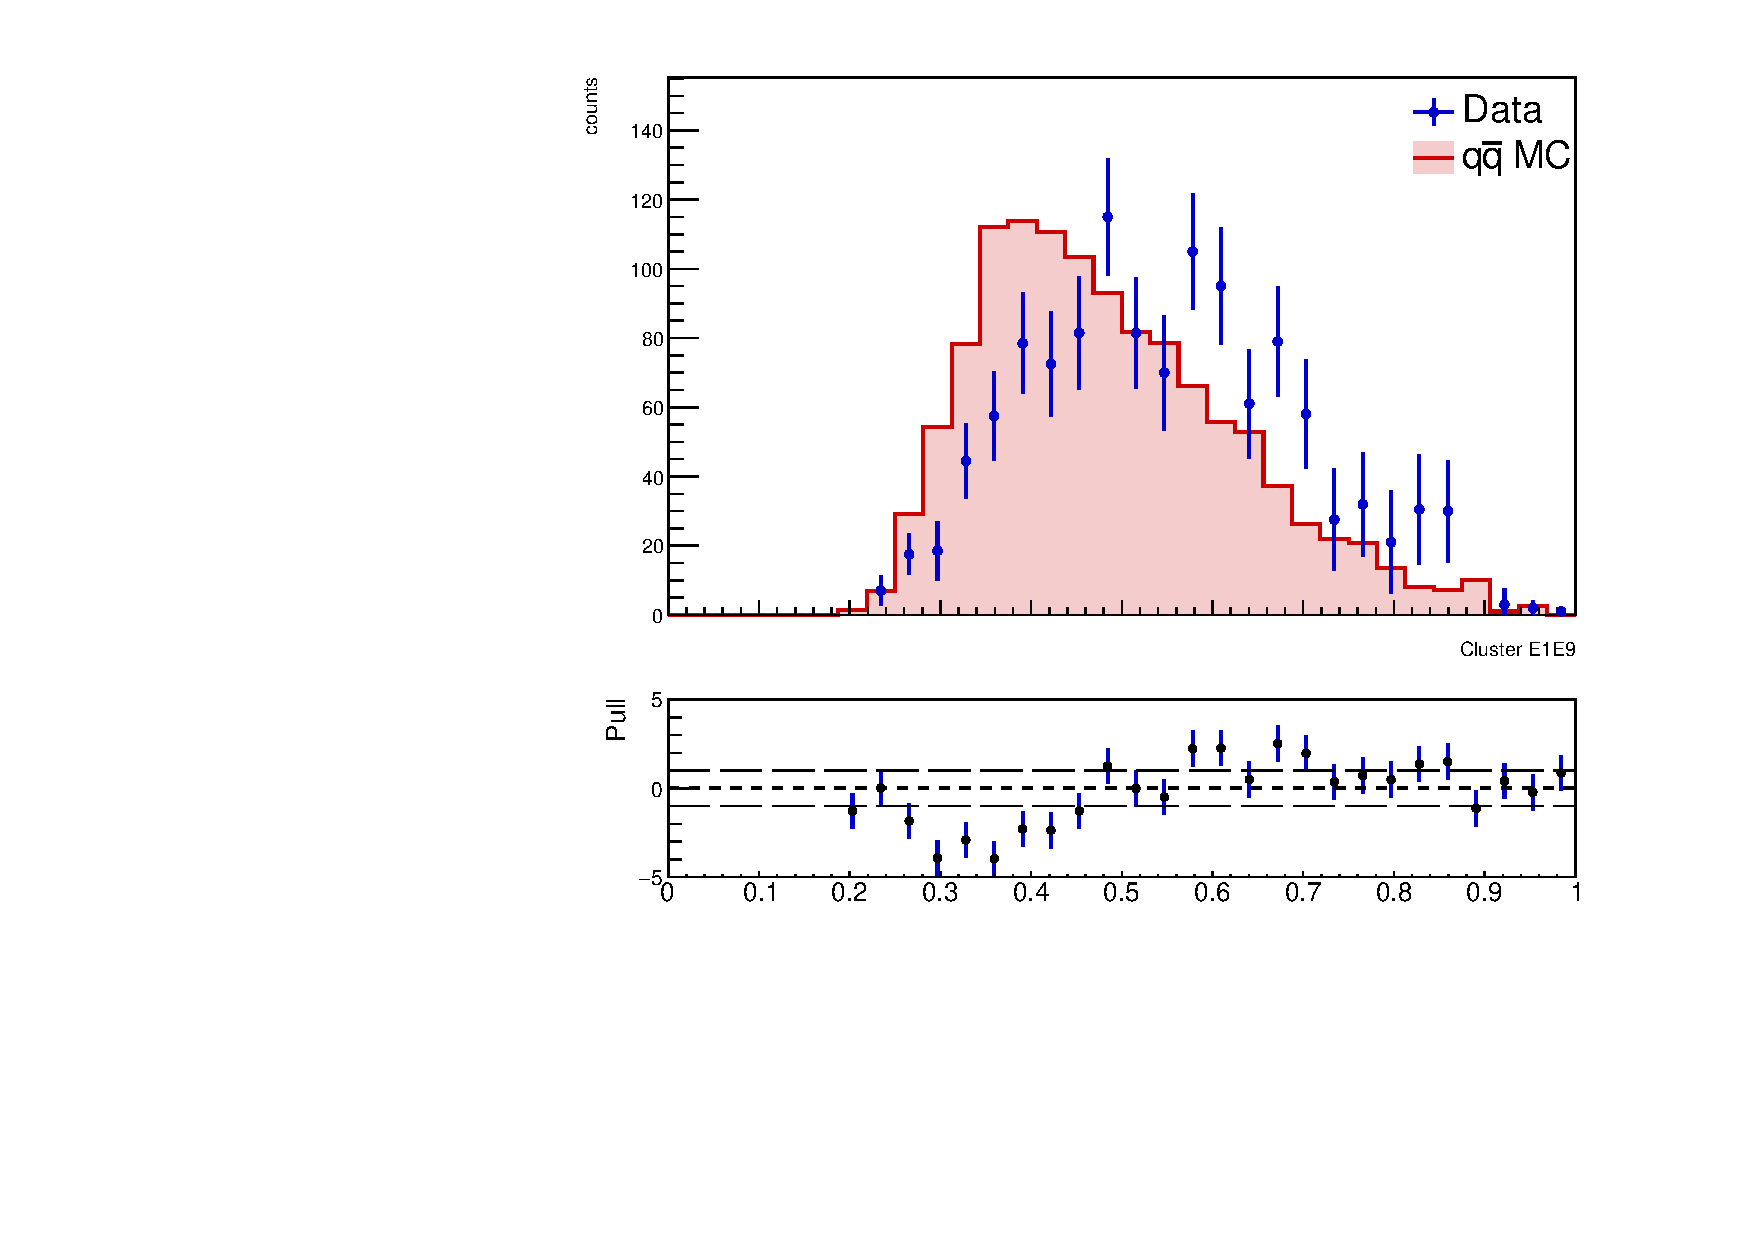
\includegraphics[width=0.49\textwidth]{nbar_data/images/dataMC_clusterE1E9_isr_pull_subtracted.pdf}
    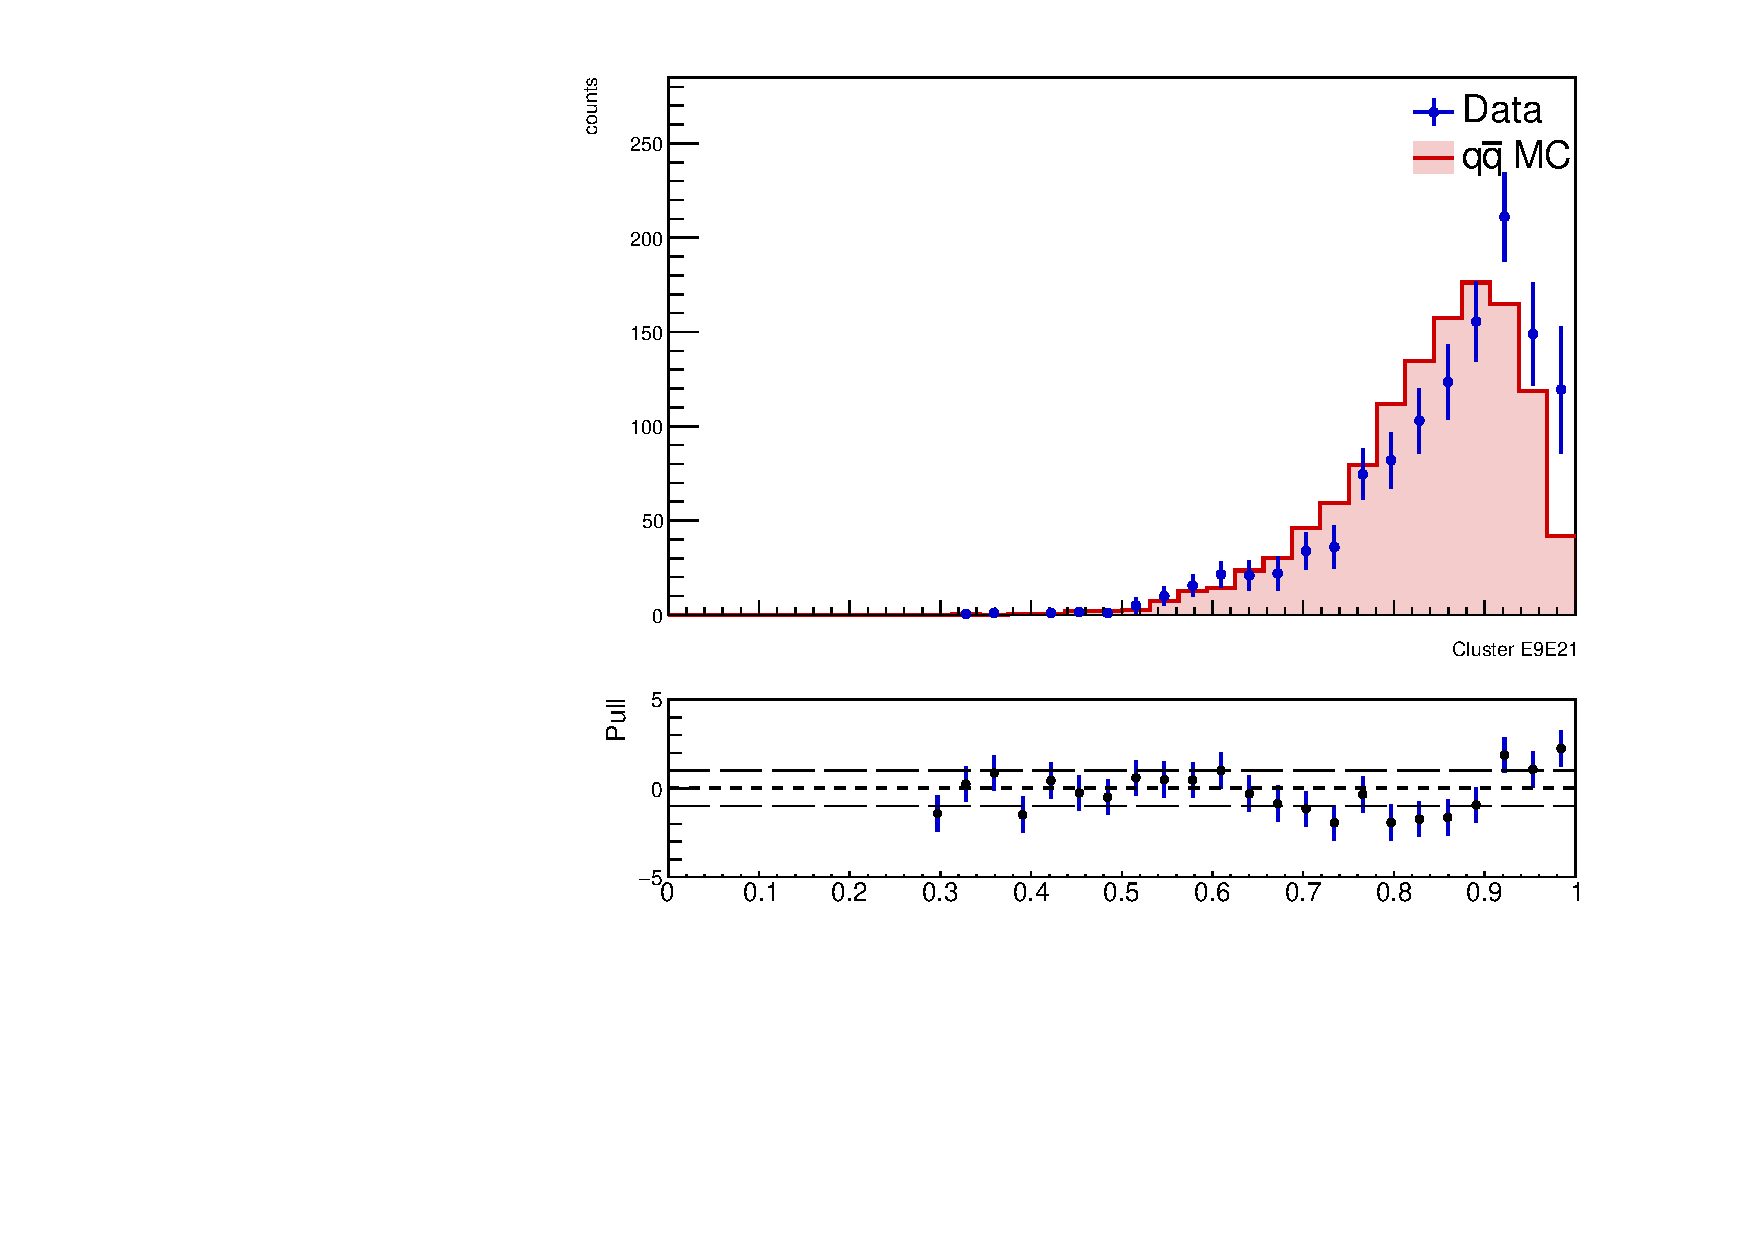
\includegraphics[width=0.49\textwidth]{nbar_data/images/dataMC_clusterE9E21_isr_pull_subtracted.pdf}
    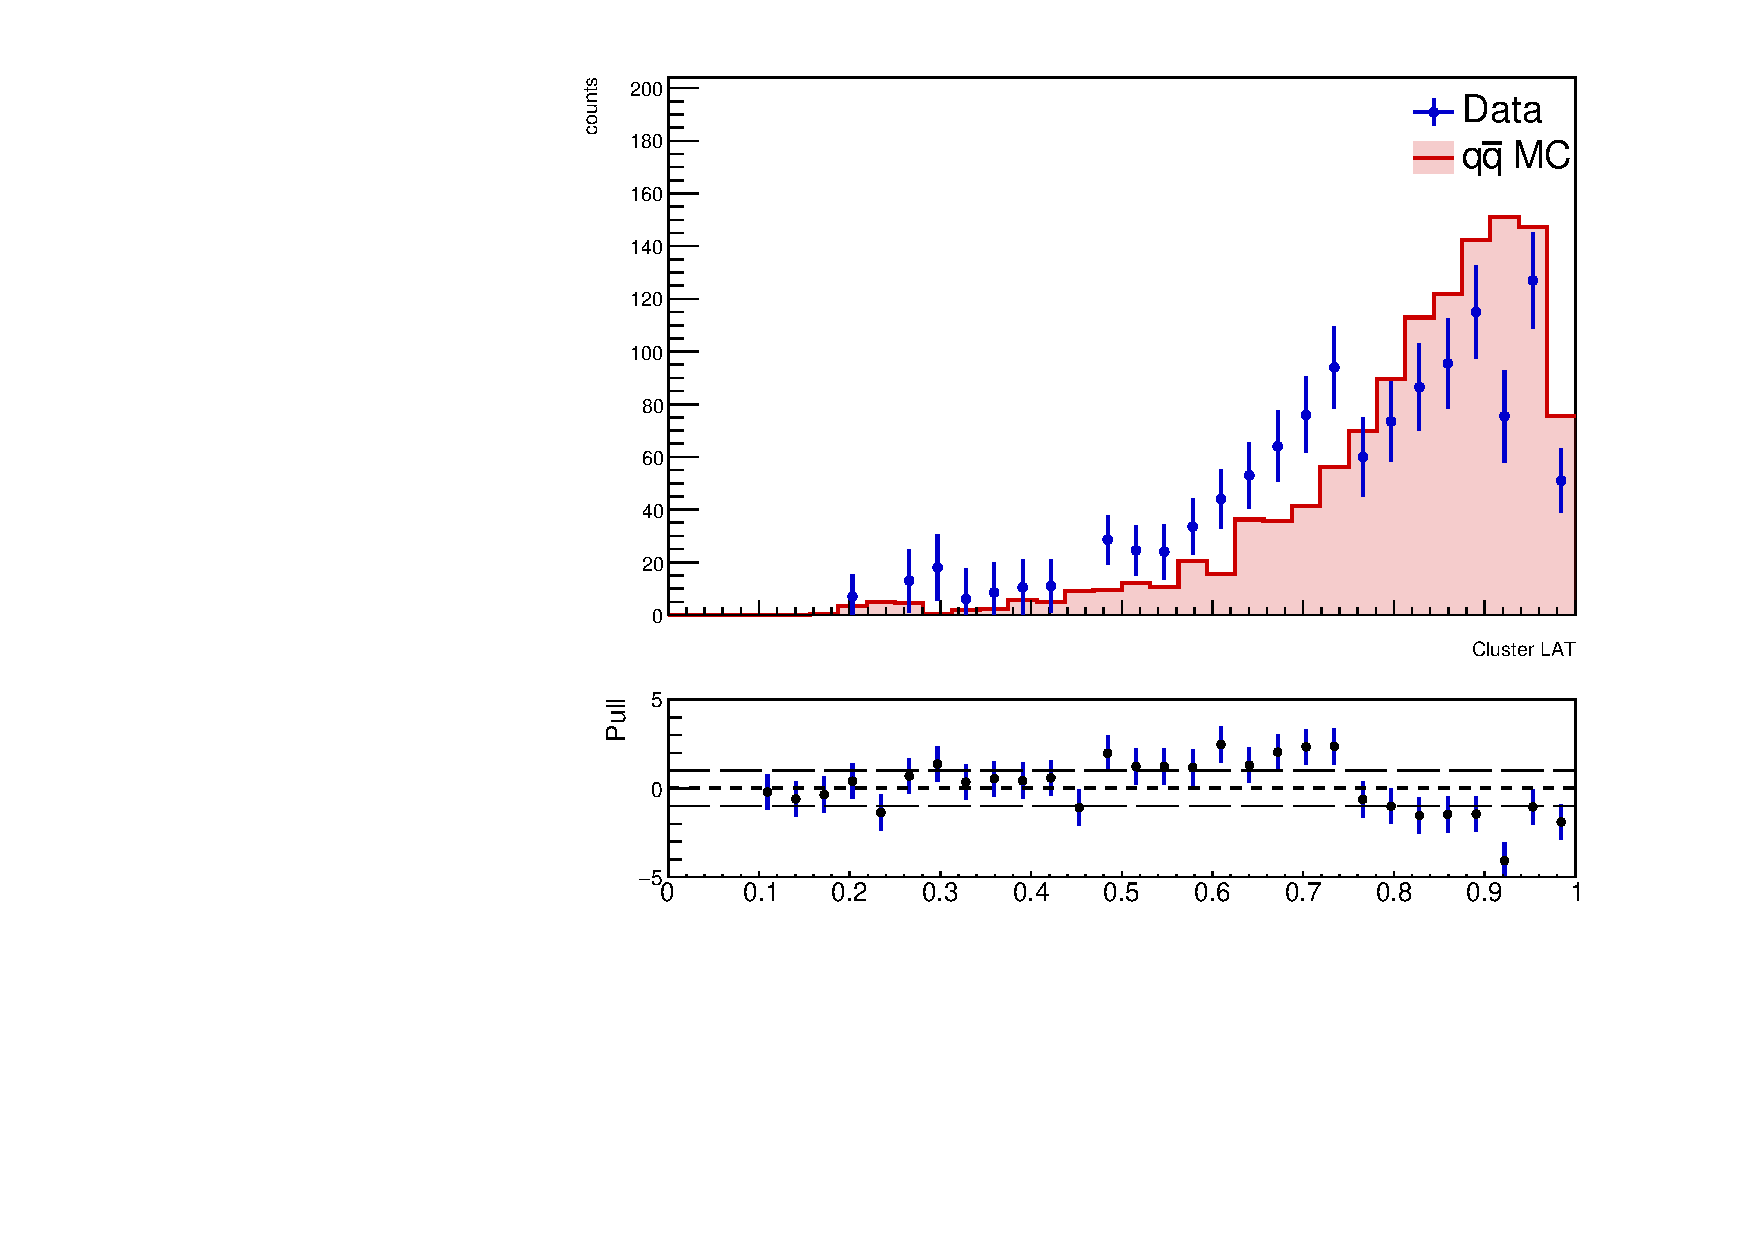
\includegraphics[width=0.49\textwidth]{nbar_data/images/dataMC_clusterLAT_isr_pull_subtracted.pdf}
    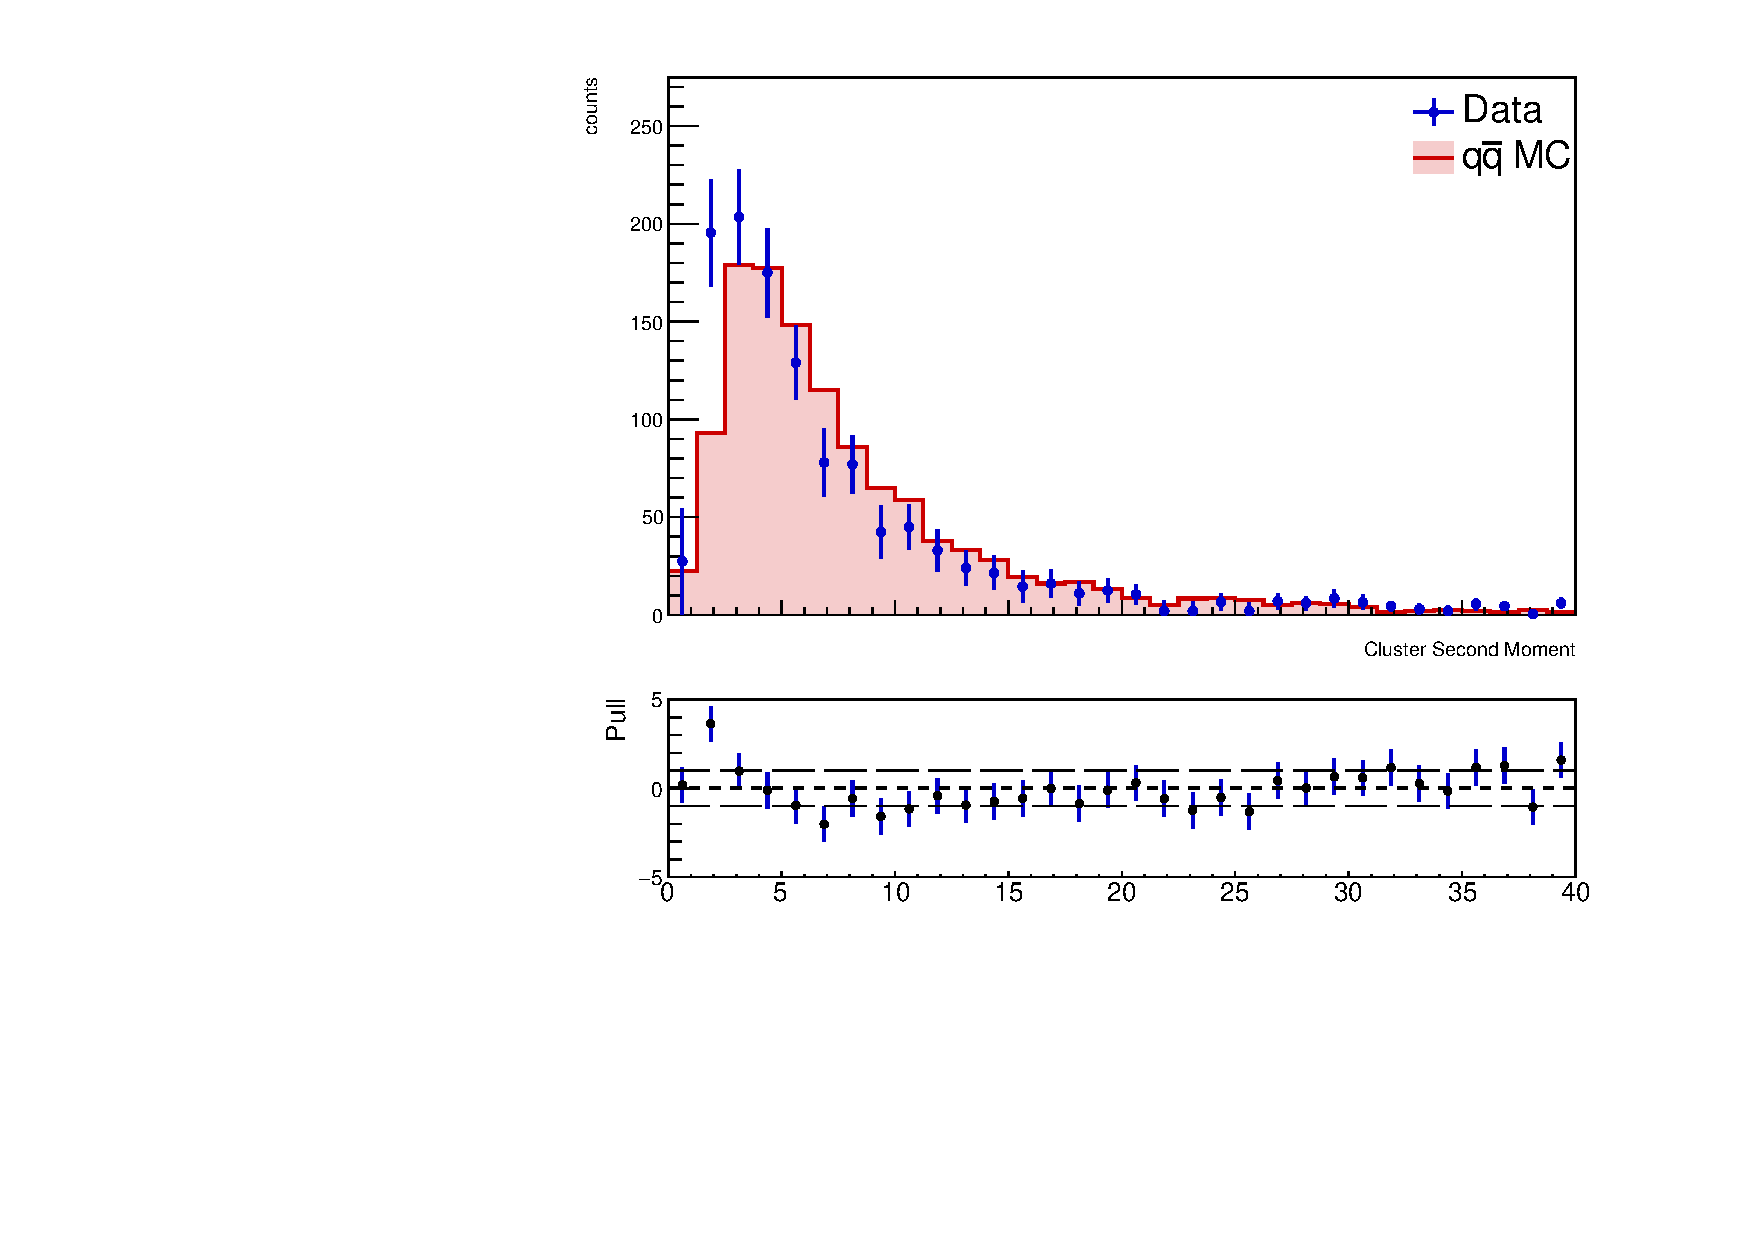
\includegraphics[width=0.49\textwidth]{nbar_data/images/dataMC_clusterSecondMoment_isr_pull_subtracted.pdf}
    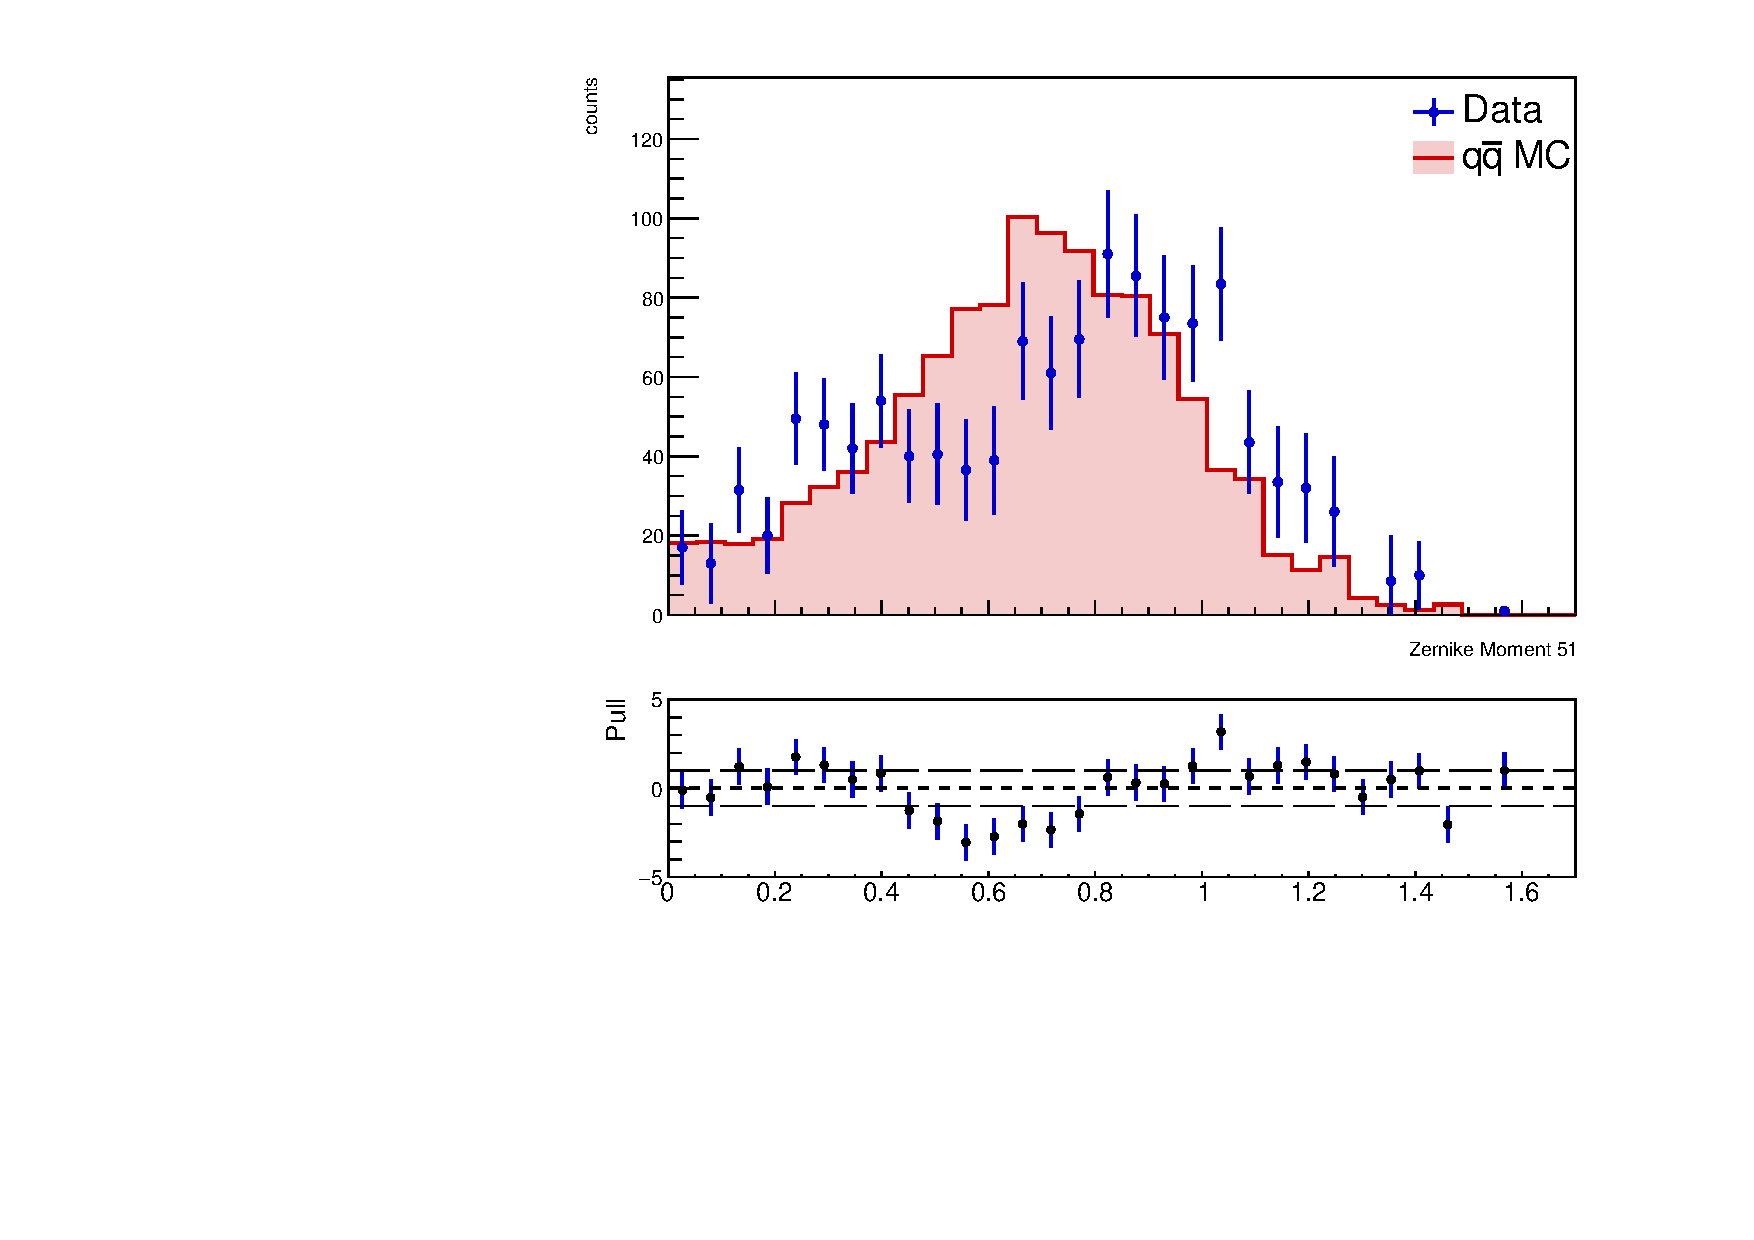
\includegraphics[width=0.49\textwidth]{nbar_data/images/dataMC_clusterAbsZernikeMoment40_isr_pull_subtracted.pdf}
    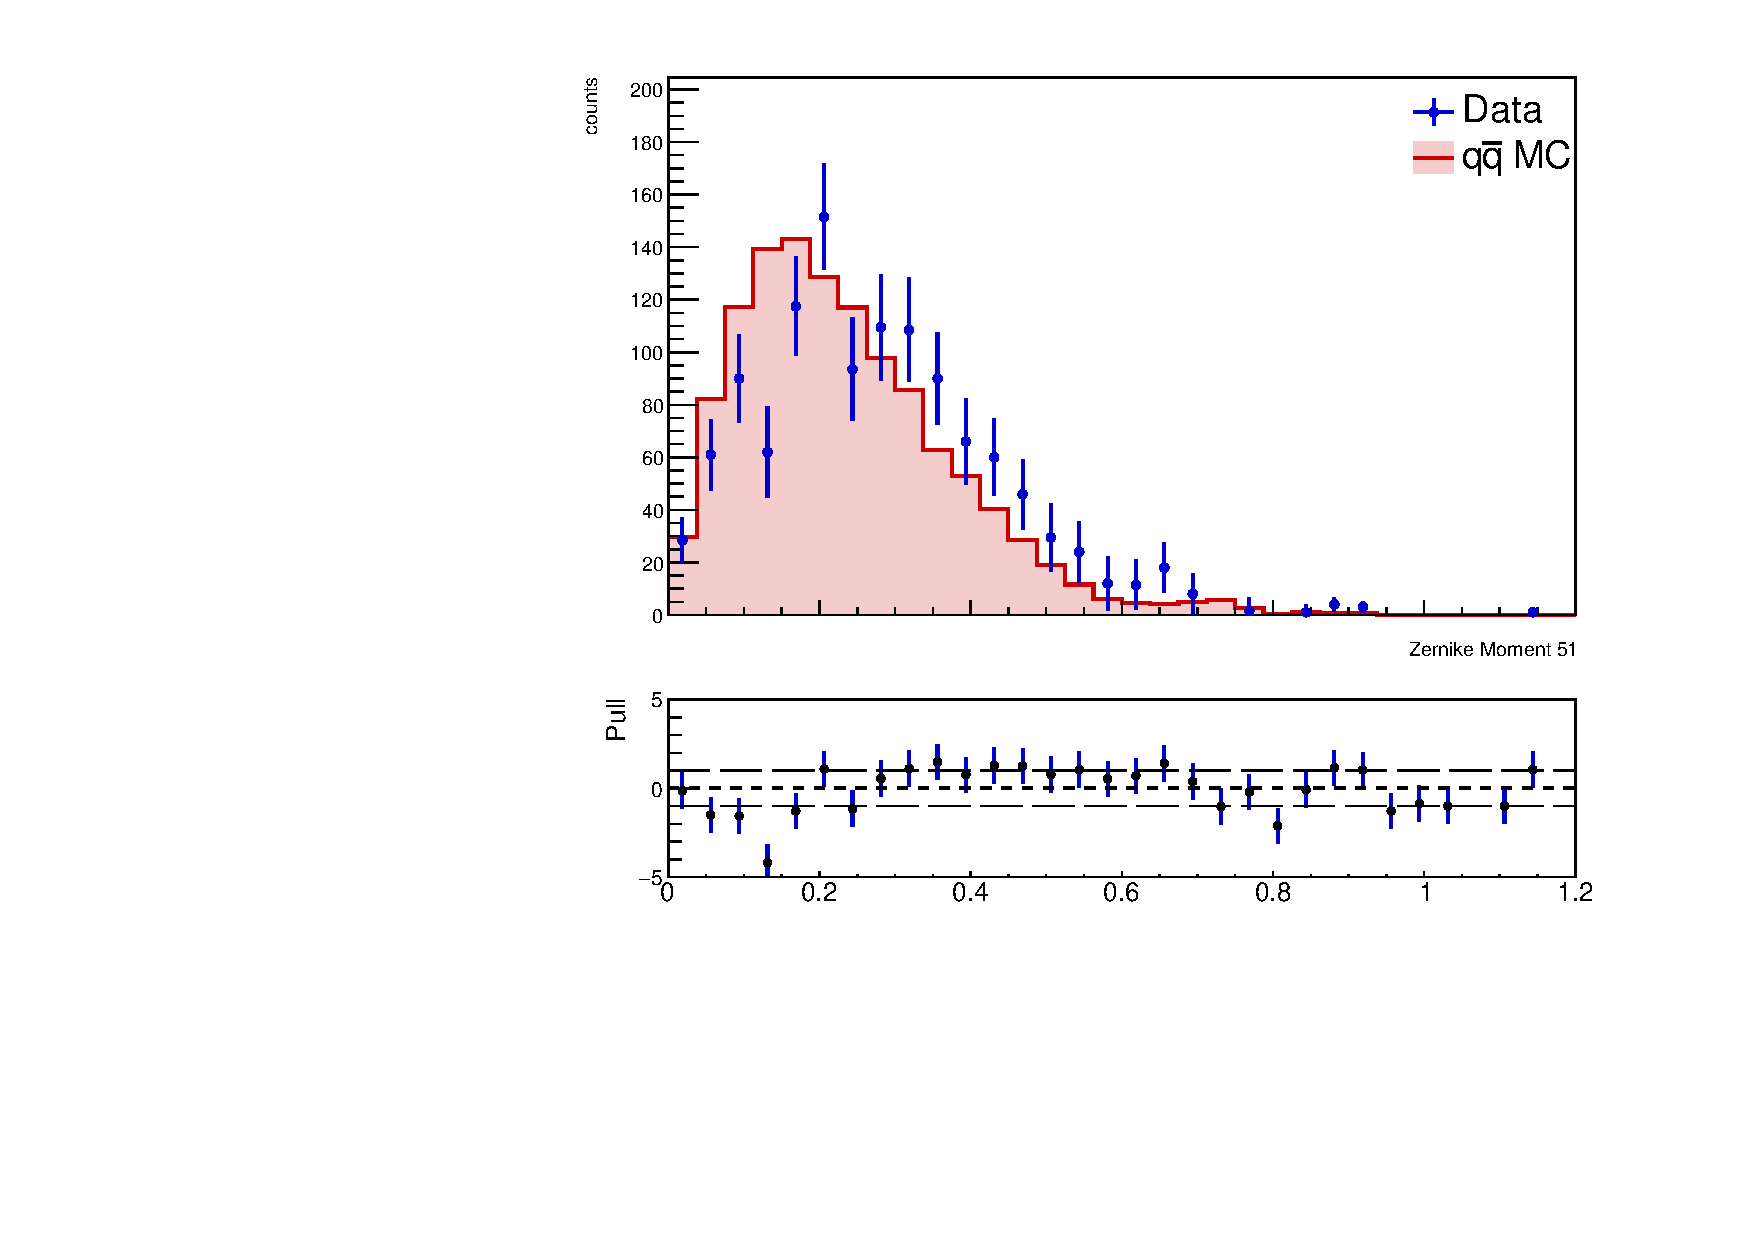
\includegraphics[width=0.49\textwidth]{nbar_data/images/dataMC_clusterAbsZernikeMoment51_isr_pull_subtracted.pdf}
    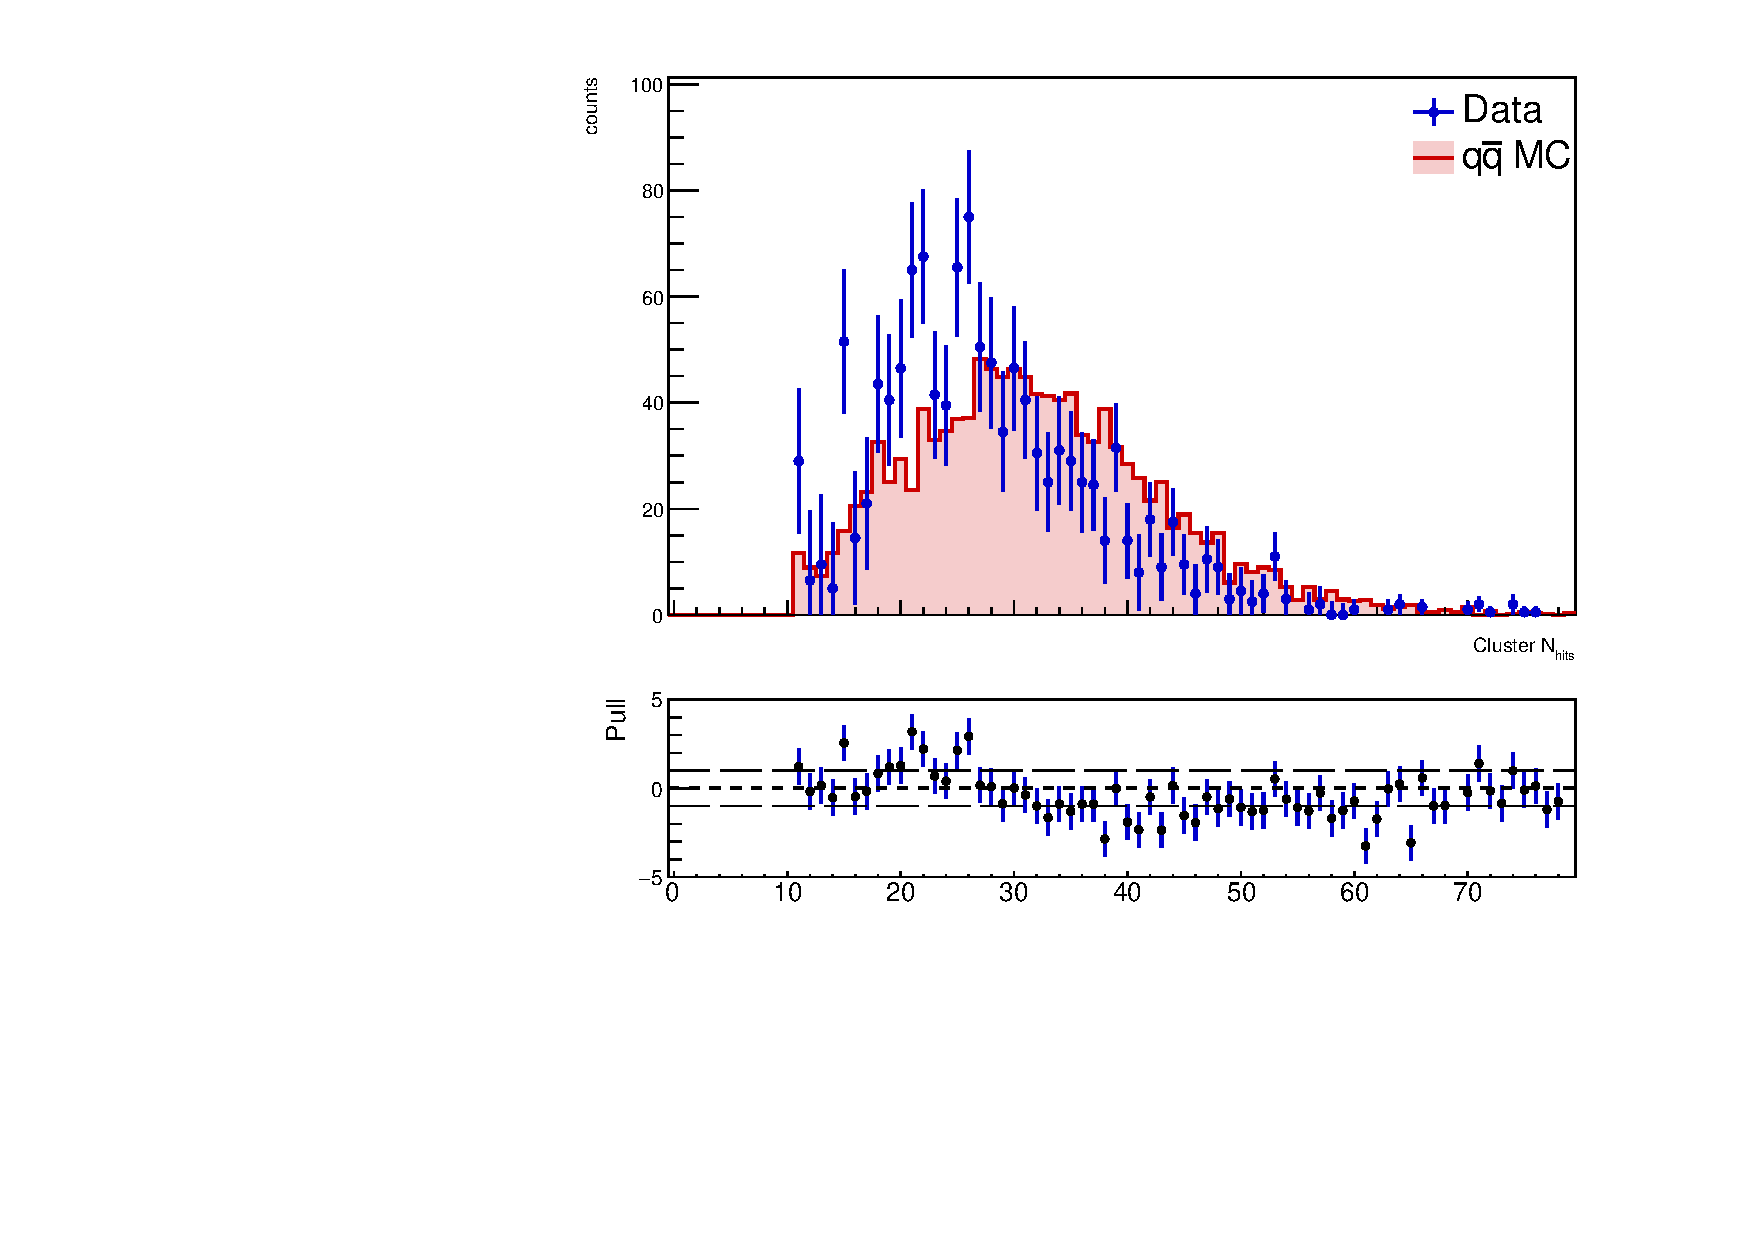
\includegraphics[width=0.49\textwidth]{nbar_data/images/dataMC_clusterNHits_isr_pull_subtracted.pdf}
   
     \caption{Data/MC agreement for reconstructed cluster variables for $\bar{n}$ candidates, in ISR case. Sidebands technique applied. Signal region: [0.8, 1.4] GeV; sidebands region: [0.2, 0.8] U [1.4, 2.0] GeV.}
     \label{fig:dataMC_isr_sid}
\end{figure}

 \begin{figure}[H]
    \centering
    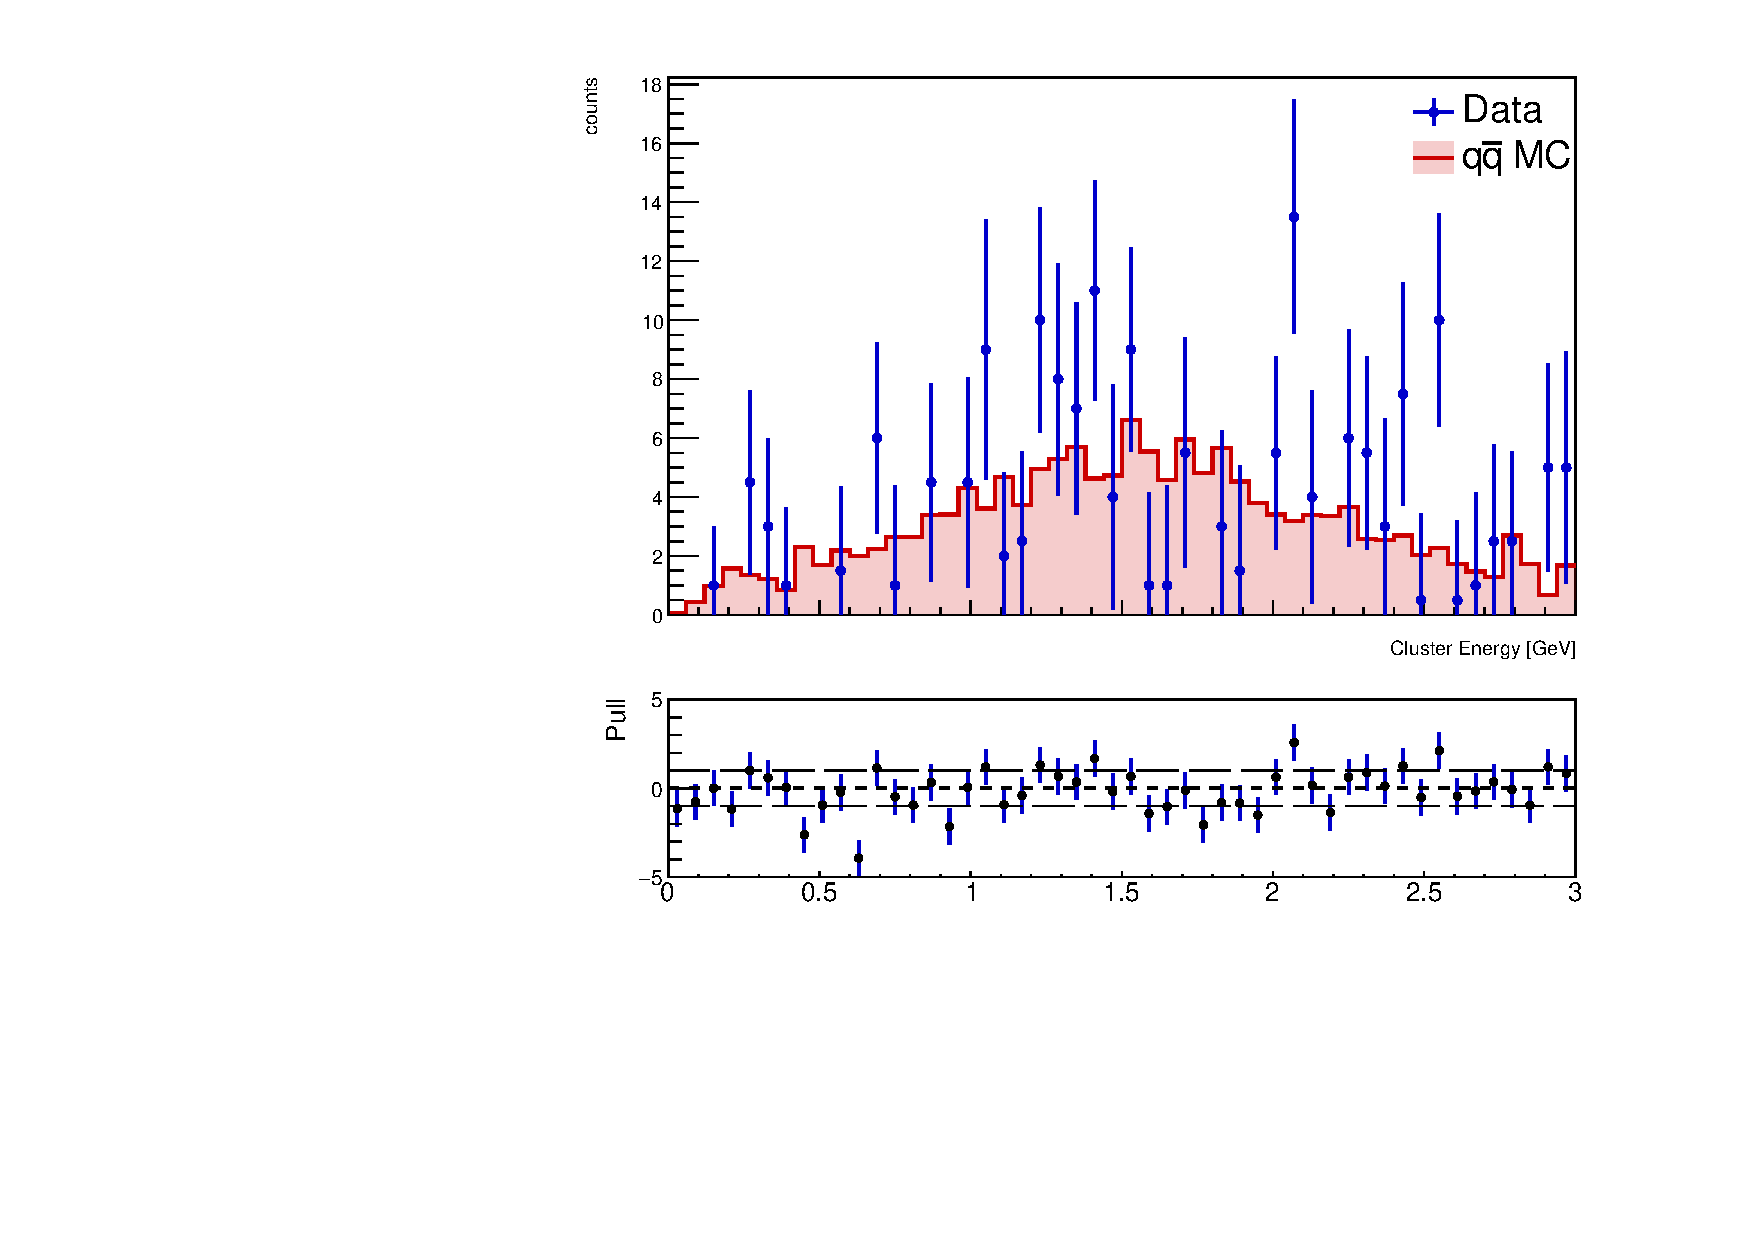
\includegraphics[width=0.49\textwidth]{nbar_data/images/dataMC_clusterE_nog_pull_subtracted.pdf}
    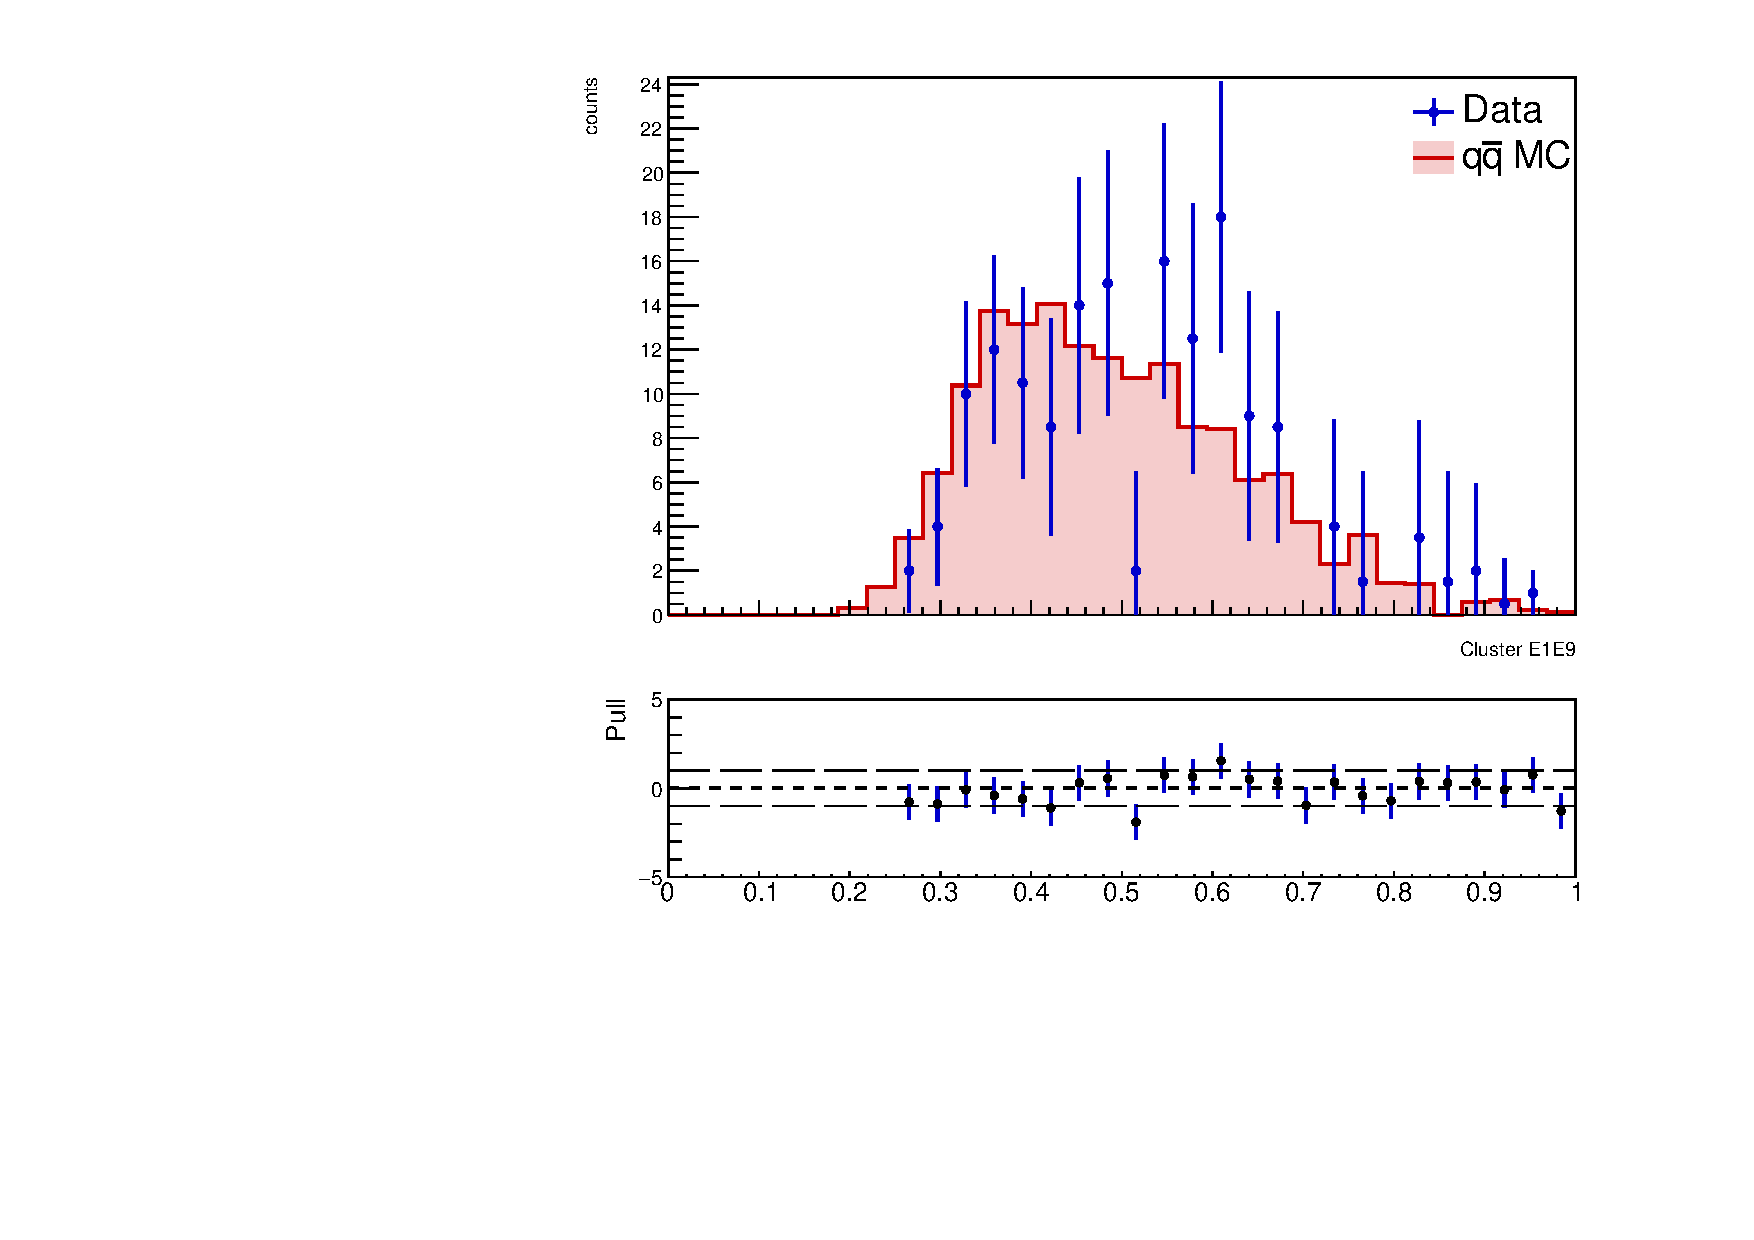
\includegraphics[width=0.49\textwidth]{nbar_data/images/dataMC_clusterE1E9_nog_pull_subtracted.pdf}
    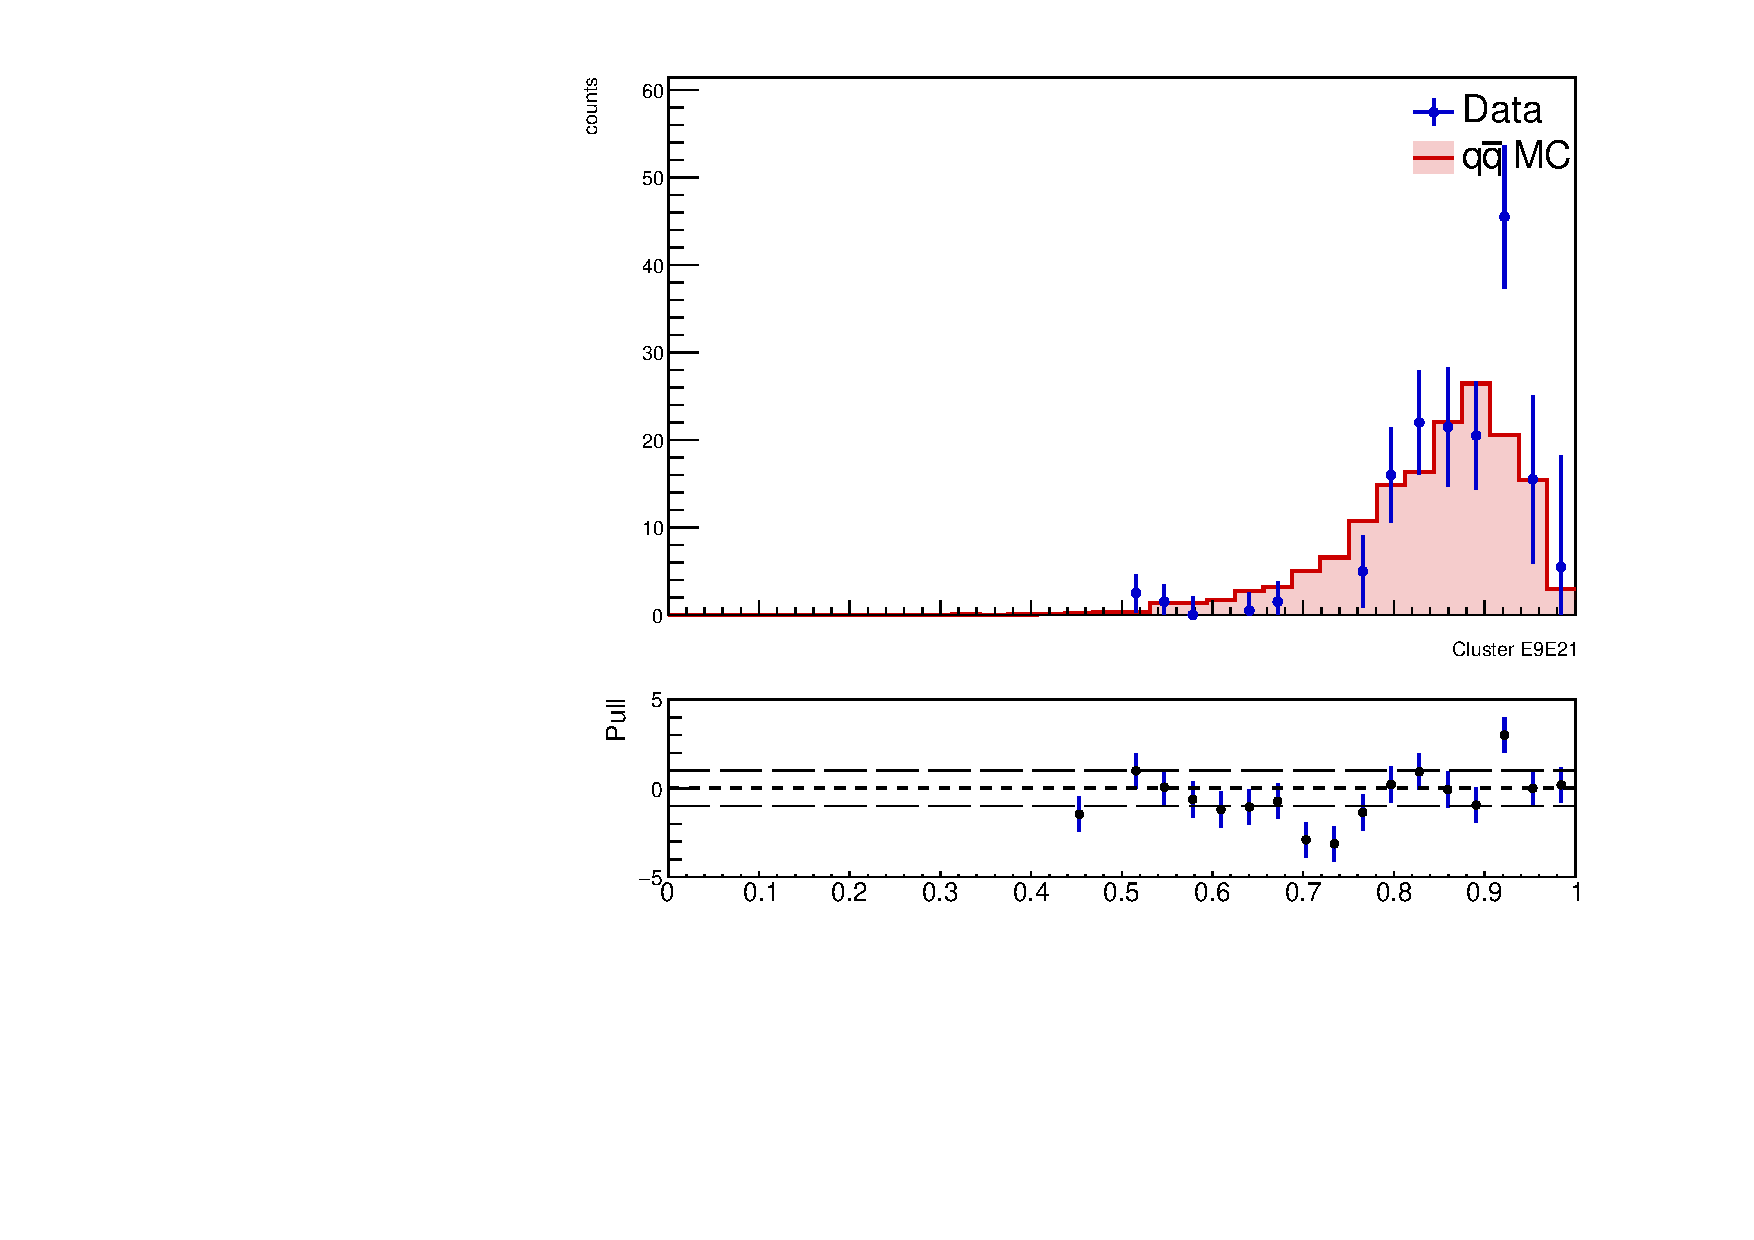
\includegraphics[width=0.49\textwidth]{nbar_data/images/dataMC_clusterE9E21_nog_pull_subtracted.pdf}
    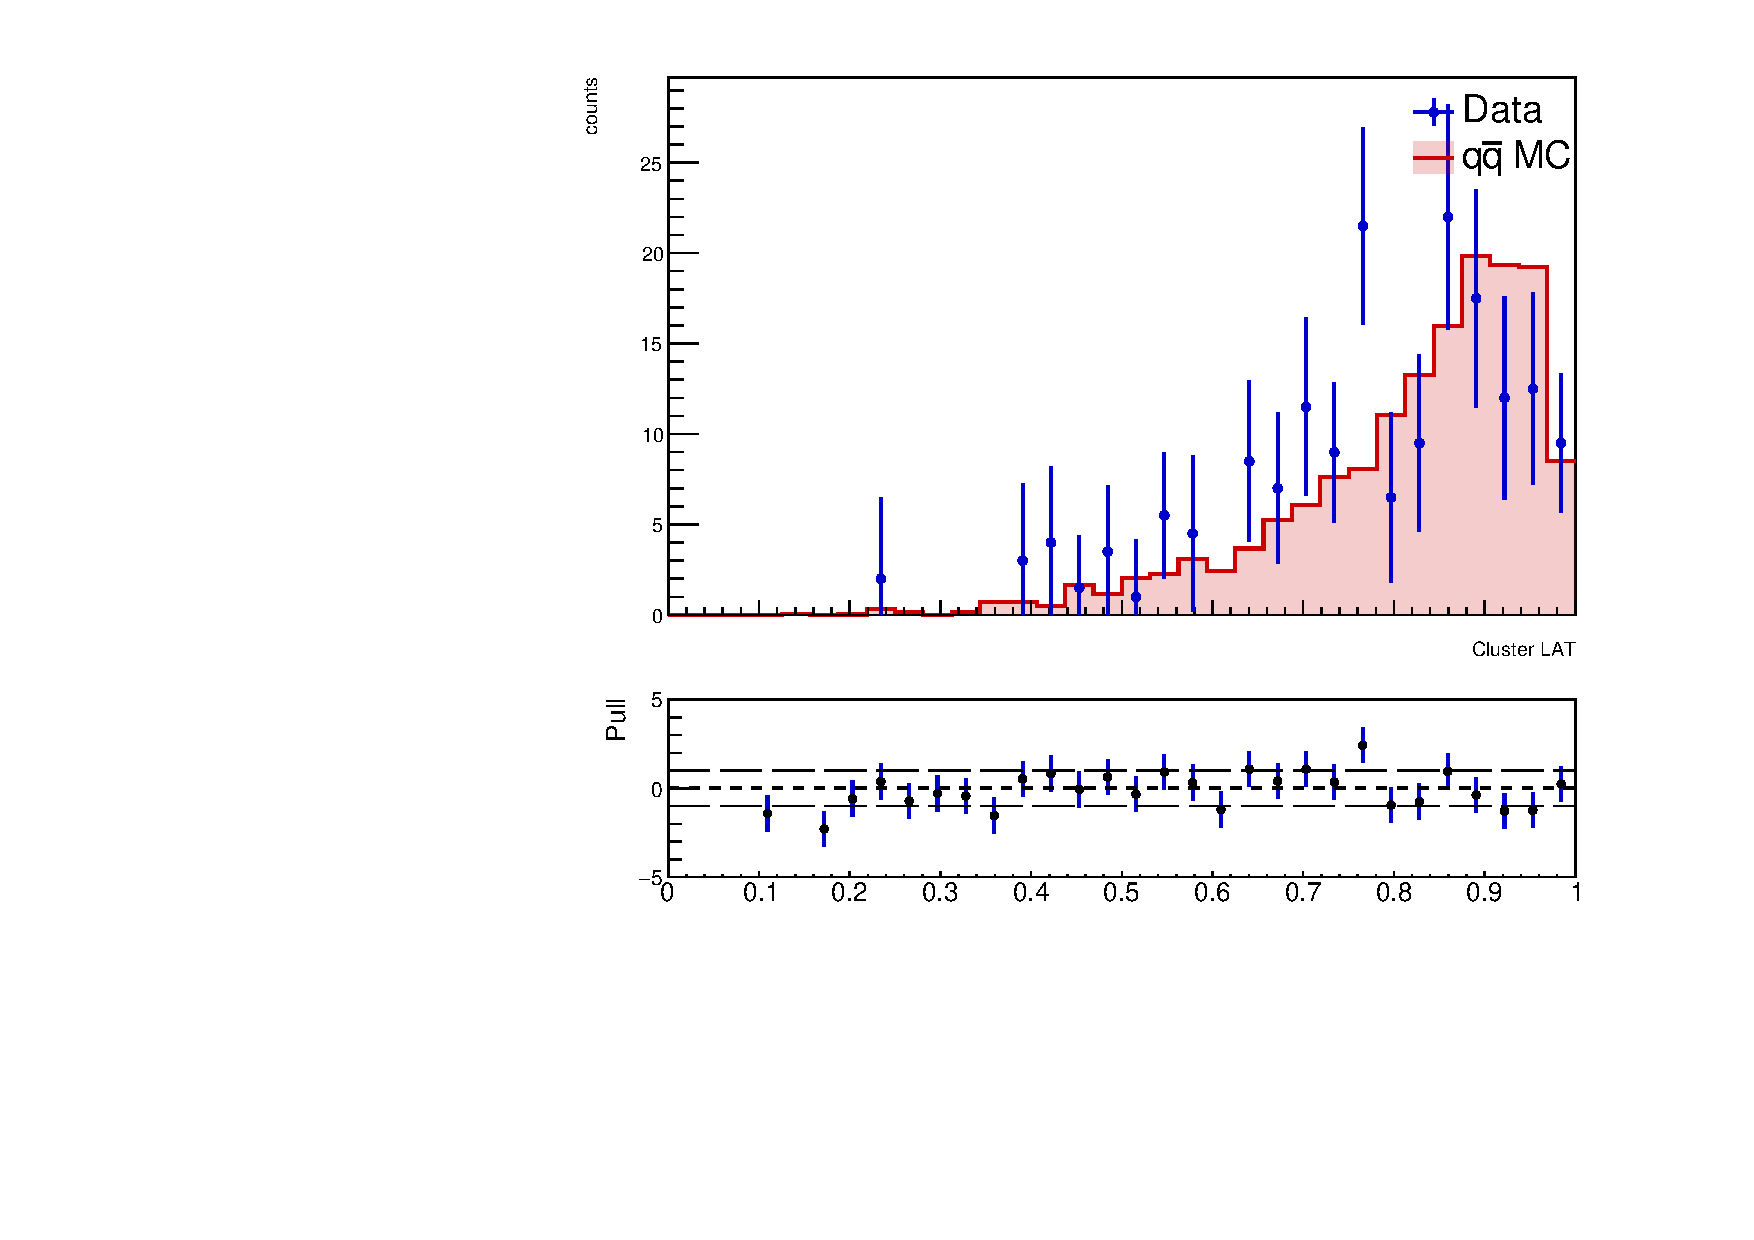
\includegraphics[width=0.49\textwidth]{nbar_data/images/dataMC_clusterLAT_nog_pull_subtracted.pdf}
    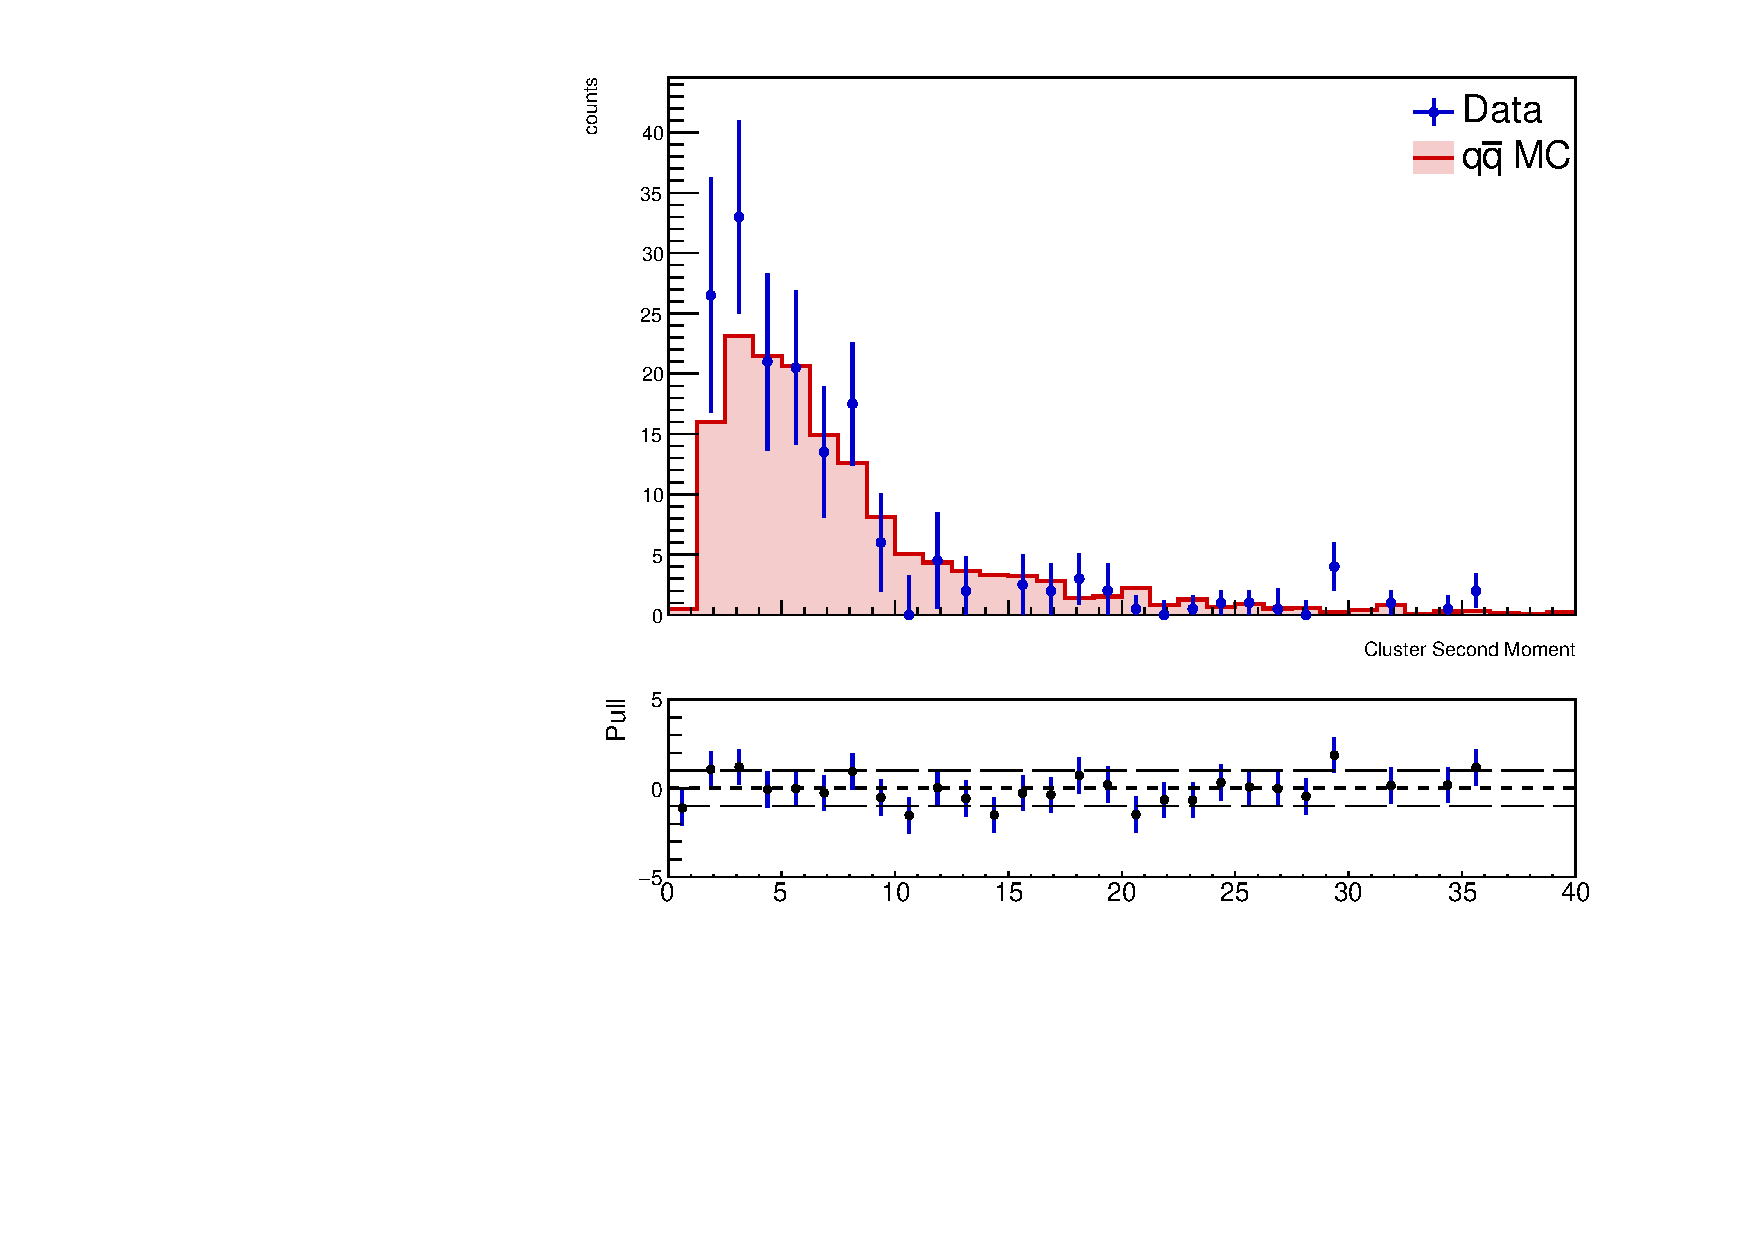
\includegraphics[width=0.49\textwidth]{nbar_data/images/dataMC_clusterSecondMoment_nog_pull_subtracted.pdf}
    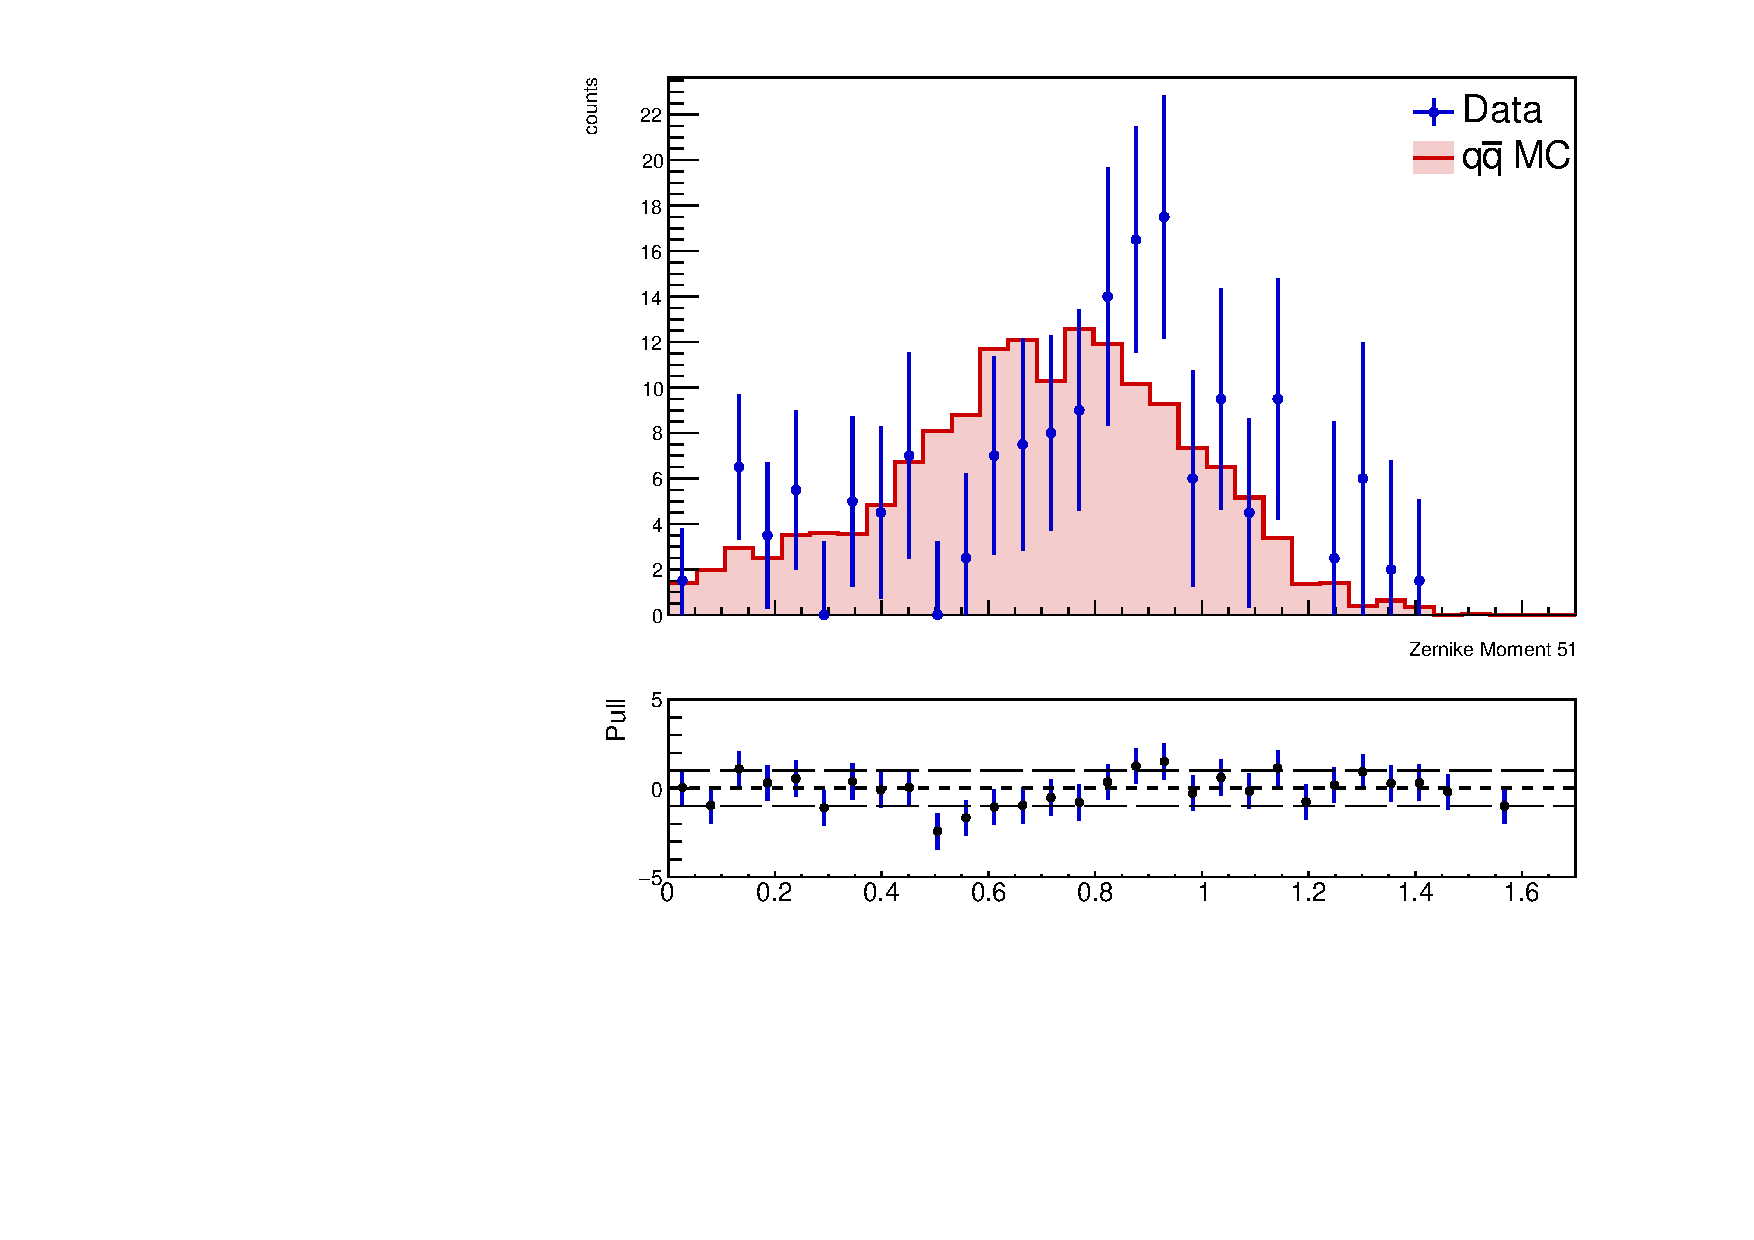
\includegraphics[width=0.49\textwidth]{nbar_data/images/dataMC_clusterAbsZernikeMoment40_nog_pull_subtracted.pdf}
    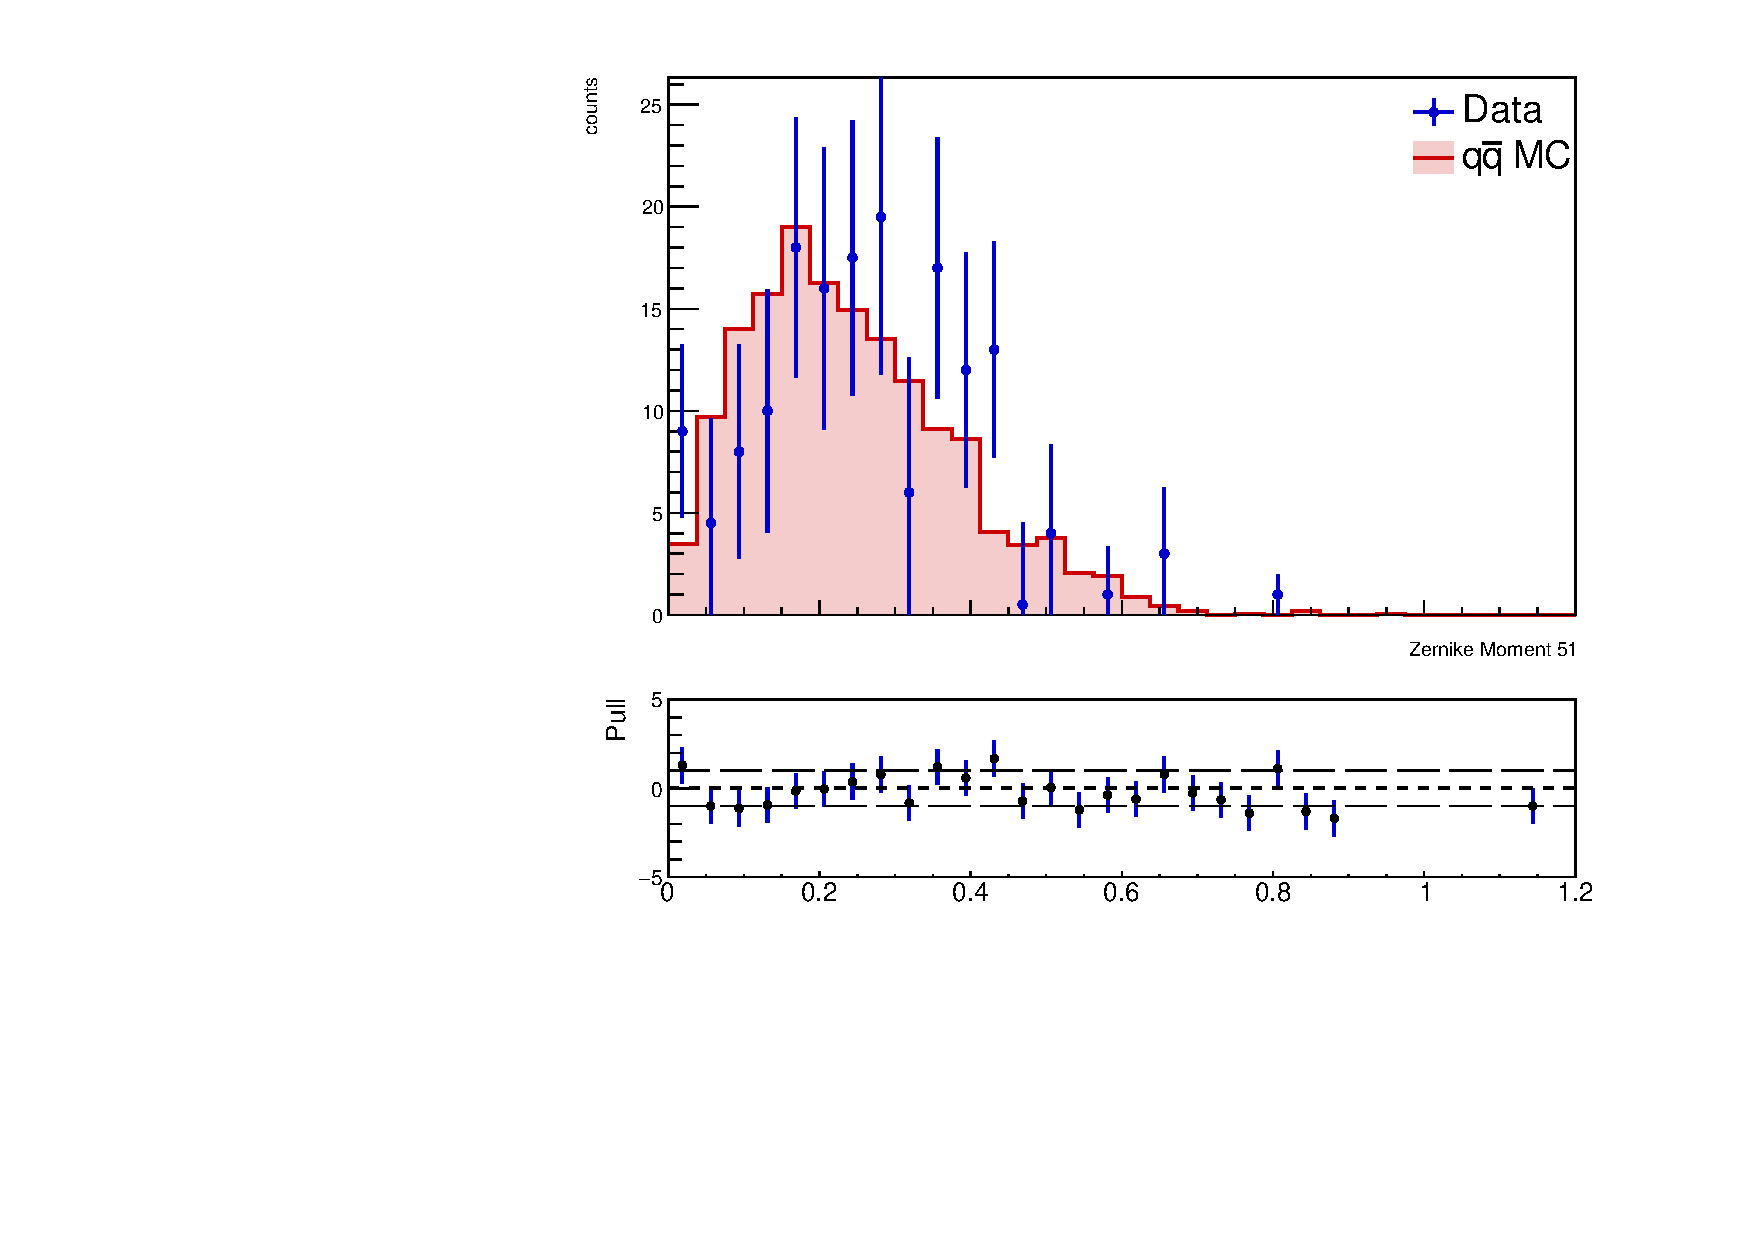
\includegraphics[width=0.49\textwidth]{nbar_data/images/dataMC_clusterAbsZernikeMoment51_nog_pull_subtracted.pdf}
    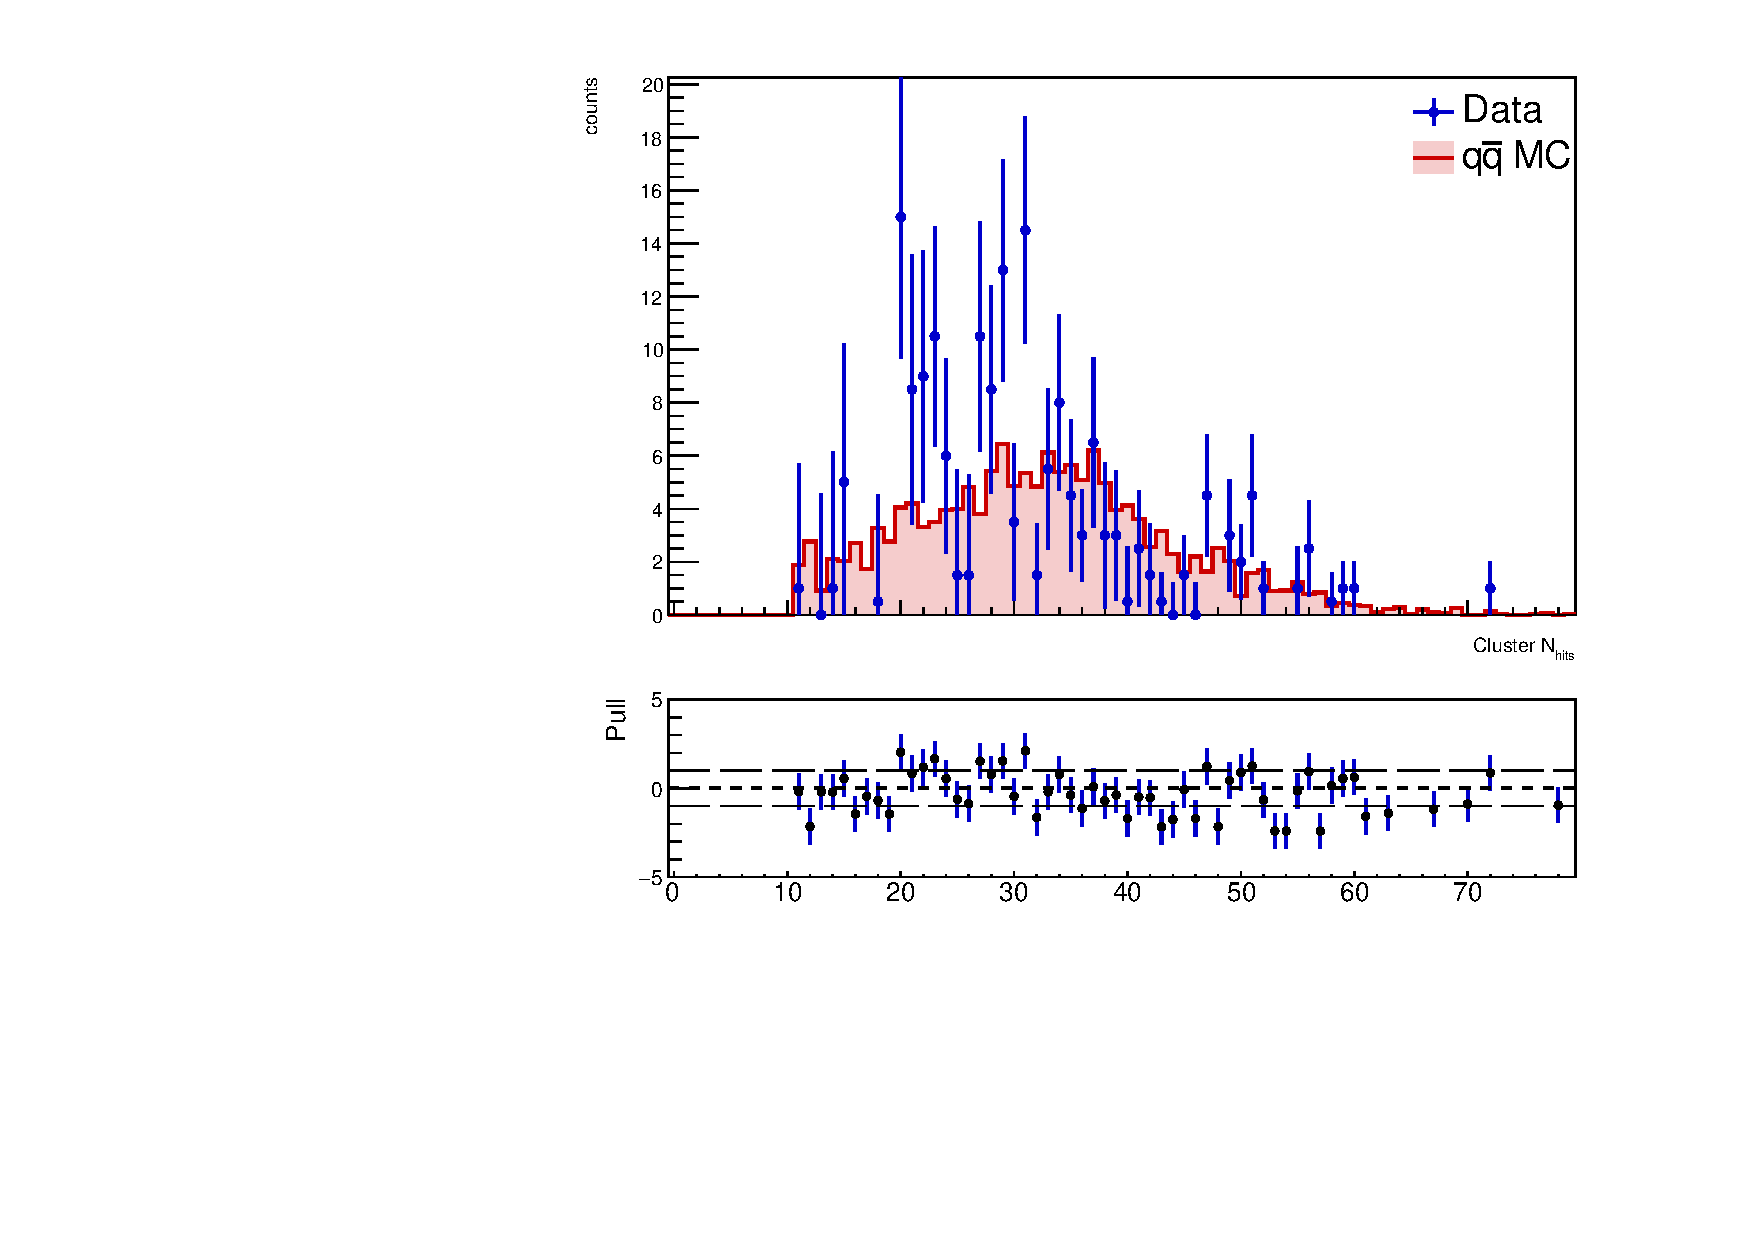
\includegraphics[width=0.49\textwidth]{nbar_data/images/dataMC_clusterNHits_nog_pull_subtracted.pdf}
   
     \caption{Data/MC agreement for reconstructed cluster variables for $\bar{n}$ candidates, in NO ISR case. Sidebands technique applied. Signal region: [0.8, 1.2] GeV; sidebands region: [0.3, 0.7] U [1.3, 1.7] GeV.}
     \label{fig:dataMC_nog_sid}
\end{figure}

\setcounter{subsection}{0} 
\part{Conclusion}

In this thesis, the $\bar{n}$ hadronic showers have been studied, with particular focus on their simulation by the Belle II software. The analysis targets the channel $e^+ e^- \rightarrow p \pi^- \bar{n}$, considering both ISR and NO ISR cases.
$\\$
$\\$
The Monte Carlo signal sample study showed good agreement between the recoil kinematic variables and the generator-level $\bar{n}$ quantities, but the reconstructed $\bar{n}$ momentum proved unreliable for estimating the true 
$\bar{n}$ momentum. Furthermore, a 1C kinematic fit improved the recoil resolution.
$\\$
Energy loss effects in primary $\bar{n}$ candidates -such as cluster split-off within the ECL and pre-showering before the ECL- have been studied. Secondary particles (mainly photons) are often misidentified as primary clusters, creating small-sized clusters that distort cluster variable distributions. The distribution of the radial distance $\rho$ of all $\bar{n}$ candidates was studied, confirming that secondary particles are produced throughout the Belle II detector -particularly in the TOP sub-detector (pre-showering) and ECL sub-detector (cluster split-off).
$\\$
$\\$
The $q\bar{q}$ cocktail study revealed the recoil mass distribution components from all cocktail channels. Therefore, additional cuts were applied, including those on the number of charged tracks in the Rest of Event (ROE) and on the $\alpha$ angle. A performance metric study using the Figure of Merit $\frac{S}{\sqrt{S + B}}$ showed that the optimal upper limit on $\alpha$ is 0.1, achieving $\epsilon_{sig} = 90\%$ and $\epsilon_{bkg} = 68\%$  signal-background discrimination.
$\\$
Furthermore, the sidebands technique was applied to obtain the $\bar{n}$ candidate cluster variables from the $q\bar{q}$ cocktail. Before subtraction, several structures -such as those observed in E1E9, E9E21, cluster Lateral Momentum, and cluster Second Moment- were present. These suggested small-sized electromagnetic showers, which were excluded after sidebands subtraction, leading to cluster variables close to those obtained in the signal sample analysis.
$\\$
$\\$
In conclusion, Data/MC agreement was assessed using pull methods. Before sidebands subtraction, cluster variable comparisons showed discrepancies beyond $2\sigma$ uncertainties between data and Monte Carlo. After subtraction, improved agreement was observed, though low statistics suggest further studies with more prevalent channels, such as multi-pion final states. The global results agree with other Belle II studies on neutral particle hadronic interactions, suggesting that further investigation of GEANT4 Physics lists for anti-neutron hadronic interactions is needed.
